\begin{filecontents*}{\jobname.xmpdata}
  \Title{Your Thesis Title}
  \Author{Matthew Asher Bardin}
  \Keywords{comma, separated, keywords}
  \Date{2023-05-31}
  \Language{en-US}
\end{filecontents*}
%
\documentclass[doublespacing]{lsuthesis}
%% To experiment with using a different document class, such as the ``book''
%% class, comment-out the prior line and uncomment the next line.
%\documentclass[10pt,oneside]{book}

%% Specify additional LaTeX packages you need.
%\usepackage{graphicx}
%\usepackage{amsmath}
%\usepackage{amsthm}
\usepackage{pdfpages}
\usepackage{url}
\DeclareUnicodeCharacter{2212}{-}
\usepackage{lsutitle}
\title{CYBERINET: INTEGRATED SEMI-MODULAR SENSORS FOR THE COMPUTER-AUGMENTED CLARINET}
\thesistype{Dissertation}
\department{The School of Music}
\soughtdegree{Doctor of Philosophy}
\author{Matthew Asher Bardin}
\degrees{B.M., Stetson University, 2017\\
  M.M., The Boston Conservatory at Berklee, 2019}
\graduationdate{August 2023}


\begin{document}

%% The command ``\frontmatter'' switches to lowercase roman page numbers and
%% unnumbered chapter headings without the word ``Chapter''.
\frontmatter

\maketitle


%% The following ``Copyright'' page is optional. You have inherent copyright
%% on anything you create, even if you choose not to include a copyright
%% notice. But if you choose to also formally register your copyright with
%% the Library of Congress, then a centered copyright notice should follow
%% the title page.
\begin{centeredpage}
\copyright\ 2023\\
Matthew Asher Bardin
\end{centeredpage}  
% Be sure to do this when sending to the library.



% \end{centeredpage}


\chapter{Acknowledgments}

First, I would like to thank my family. Without their continued support, I would not have been able to make it into graduate school, let alone be finishing my dissertation project. Thank you from the bottom of my heart Mom, Dad, Michael, Melanie, and everyone else. 

I would also like to thank my various professors and mentors that I have had the pleasure of working with over the past decade. From building a general approach to music and technology in my undergraduate studies, to finding my passion while finishing my Master’s degree in Boston, to the guidance I received on this project; the advice I have received from these people has helped me to not only build a strong knowledge base, but achieve the confidence to present my work and my art to the world.

Lastly, I would like to thank my cat, Bean. Regardless of whether she was in the way; she always made a spot on my desk to join me while I was writing. When in doubt, I would always defer to her expert opinion on any matters related to ear-scratches, pets, and wet food. Thank you, Bean.

\vspace{10mm}

\begin{center}
    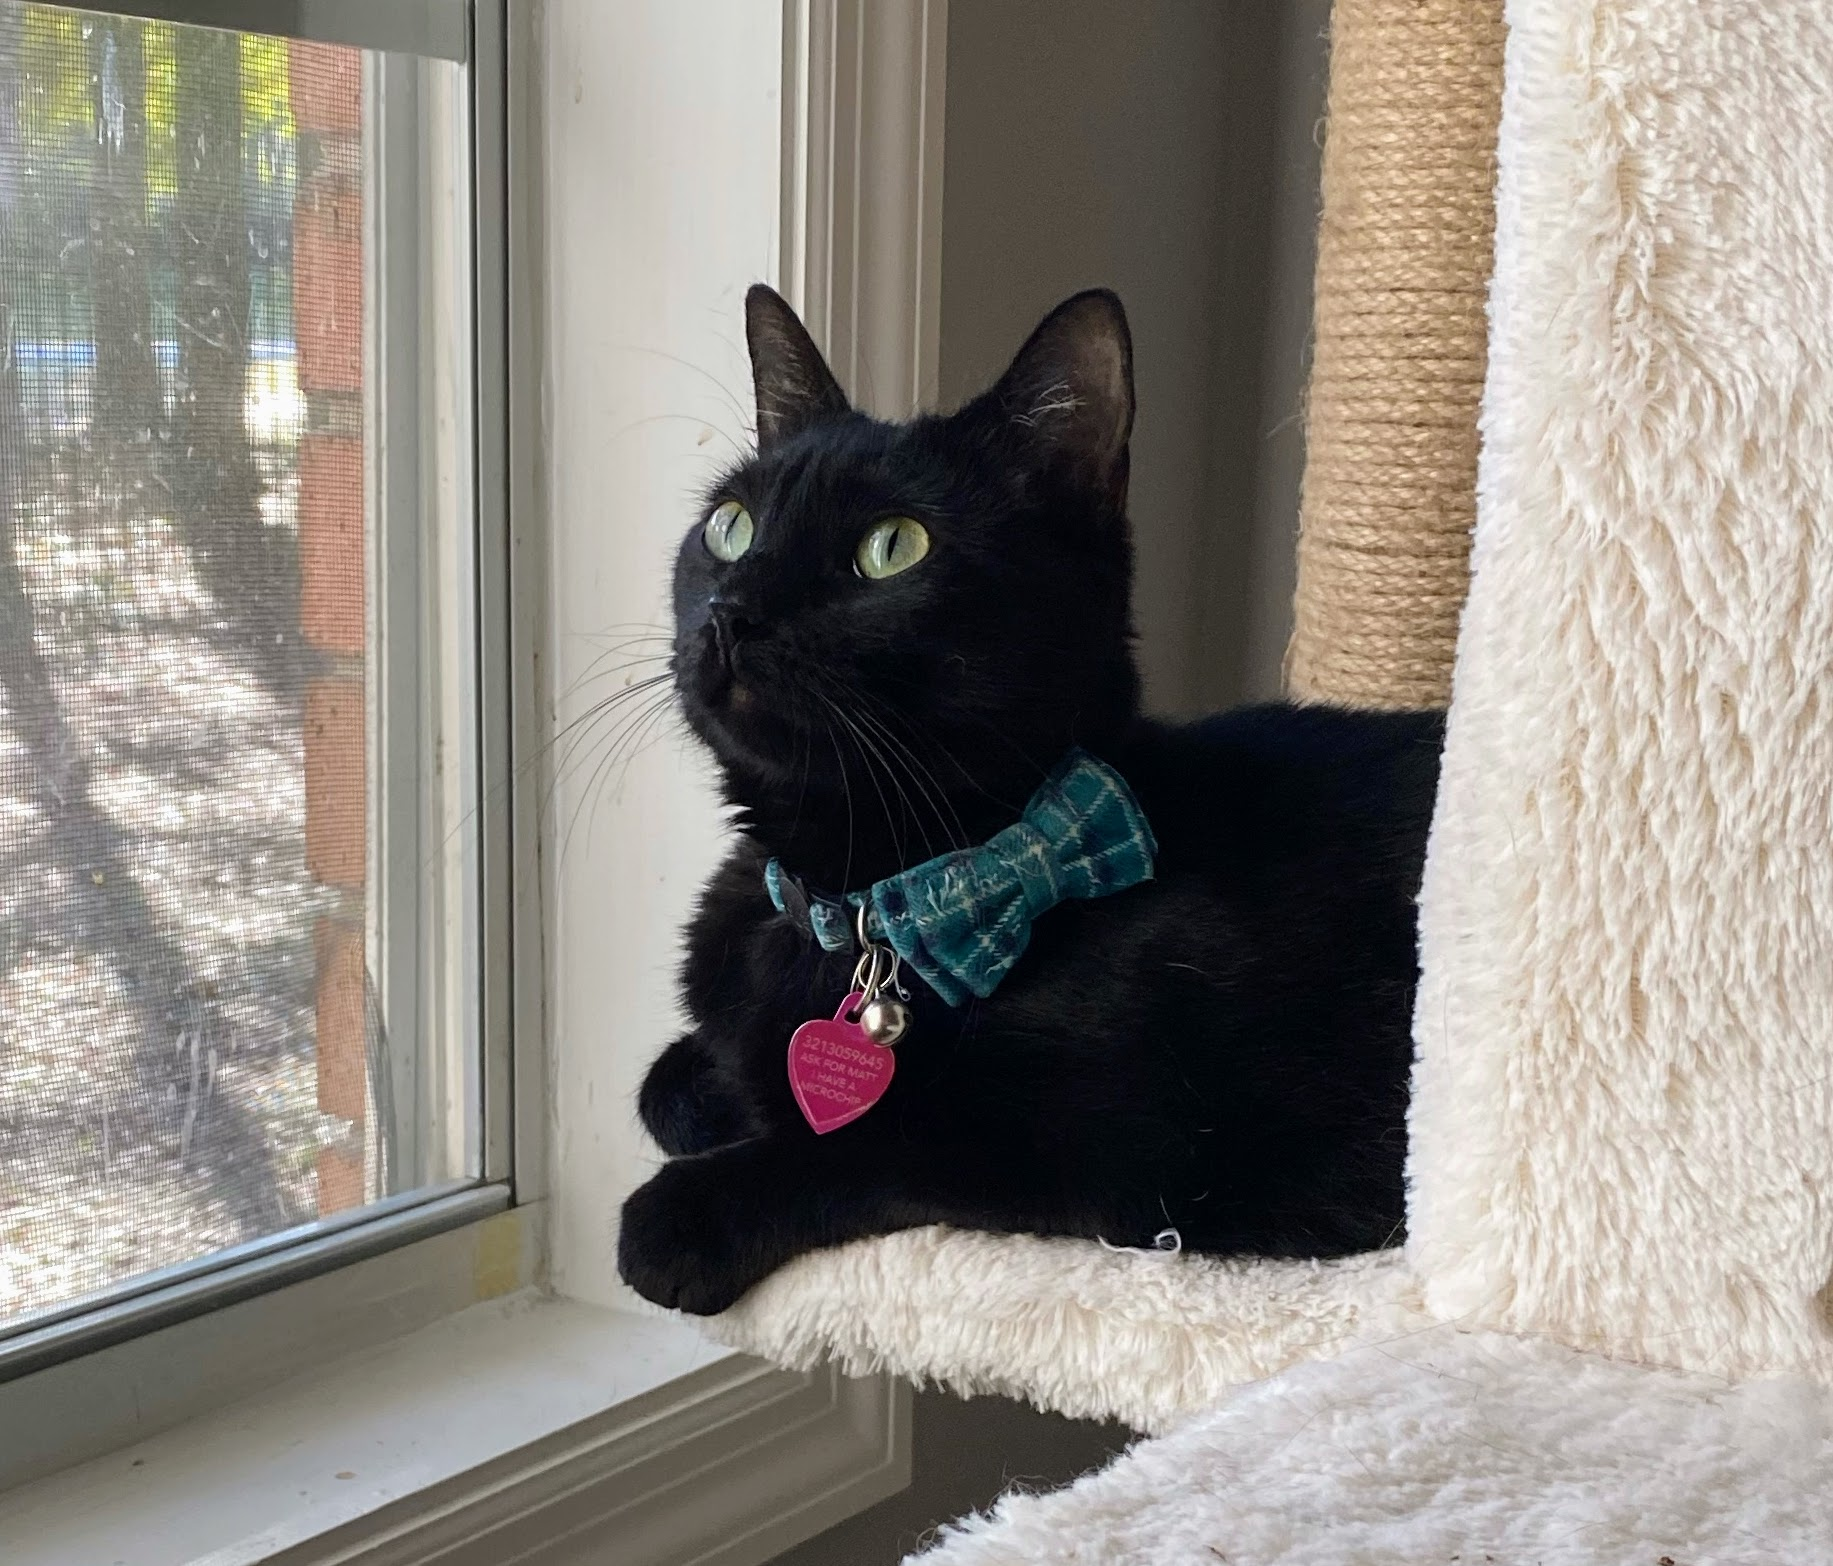
\includegraphics[scale=0.12]{bean.jpeg}
\end{center}



\tableofcontents



 \listoffigures


\chapter{Abstract}

% The ``abstract'' is required and is limited to 350 words.

Augmented instruments have been around in some form for almost as long as instruments, but have had a relatively recent explosion in presence and capabilities due to the progression of technology through the 20th and 21st centuries. One potential use of augmented instruments is to control audio processing on a computer utilizing Max or other software environments. By being able to control the music natural expressive means, the performer and composer are able to experiment with a verity of ways to make sound. A performer is able to hear their sounds and adjust their playing in order to change them in real time, or the sounds are able to react to a performer's movements automatically. This act brings up the idea of cybernetic music, wherein the music being created can influence the creation of future music. One new instrument that works to combine these two ideas is the Cyberinet.

The goal of this project is to provide a method of computer-enhanced performance to the solo clarinetist with minimal interference to their normal performance practice. A performer utilizing the Cyberinet is to be able to be able to seamlessly switch between a traditional performance setting and an augmented one. Towards this, the Cyberinet is a hardware replacement for a portion of a clarinet containing a variety of sensors embedded within the unit. These sensors collect various real time data gyroscopic data of the performer and air flow within the instrument. Additional sensors can be connected to the Cyberinet to further expand its capabilities, which allows for the unit to become customizable based on various performance needs. This data is then transferred to a computer via Bluetooth connectivity in order to use the data in any number of potential electroacoustic performance settings. 

In order to explore these new relationships, in addition to the instrument itself, a collection of Max objects designed from the ground up to utilize the Cyberinet’s data in musical contexts has been developed. These Max objects were utilized in the performance of four new compositions for the Cyberinet in the spring of 2023.

%% The command ``\mainmatter'' switches to regular page numbers and
%% chapter headings that include the word ``Chapter''.
\mainmatter


% \chapter{Introduction}
% \label{chap:intro}




\chapter{Defining the Cyberinet}
The idea of augmenting an instrument has been around for almost as long as instruments themselves. In the modern sense, an augmented instrument can be defined as any acoustic instrument that has had an increase in functionality due to additional, usually electronic, additions to the instrument. It is important to note that in order to be an augmented instrument and not something completely new, the original functionality and capabilities of the original instrument remain intact\cite{miranda_Wanderley_instrumentControl_2006}. For example, an electric guitar can still function as a guitar even when not utilizing the built in amplification.

This chapter will discuss various concepts and examples in creating augmented instruments, going back several hundred years until the early 21st century. The second section will discuss concepts of Cybernetic music and composers who have utilized those concepts in their own work. All of this will lead into the design and Cybernetic intentions of the Cyberinet, a new Augmentation for the B-flat clarinet.


\section{Augmented Instruments \& Music}

\subsection{Pre-20th Century Augmented Instruments}
In many contexts, the idea of augmenting instruments is viewed as a relatively new practice. While there has been an increase in the number of augmented instruments, especially those with electronic and computer-controlled augmentations over the past century, the concept of improving the capabilities of instruments proceeds the electrical manipulations by centuries.

To clarify this viewpoint, I have three main examples. The first is the development of brass mutes. By itself, a brass mute serves as an entirely mechanical and removable augmentation for the instrument it was designed for. A trombonist utilizing a mute has a greater range of timbral options when compared to a performer not utilizing a mute. While not the first instance of a mute being used in modern music, the score to Montiverdi's 1509 opera \textit{Orfeo} opens with this distinct timbre.

\begin{figure}
    \centering
    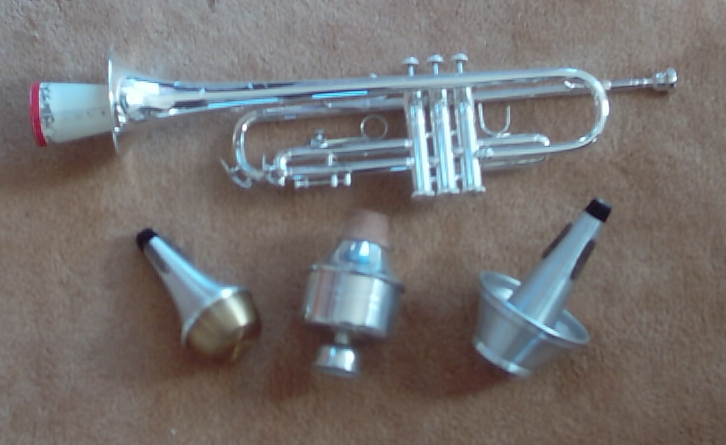
\includegraphics[scale=0.35]{diagrams/TrumpetMutes.jpg}
    \caption{A variety of trumpet mutes}
    \label{fig:tptmutes}
\end{figure}

Modern versions of brass mutes have been made for every common-place brass instrument, and many variety of mutes have been created to allow for a greater variety of timbre possibilities in both performance and orchestration settings. While different mutes will vary slightly based on the instrument and type, they all generally work by achieving one goal. All brass mutes serve to absorb a portion of the instrument's produced sound waves, filtering the sound, and changing the timbre. Some mutes such as cup and bucket mutes serve to block the sound waves in the air. Harmon mutes create a resonating chamber to change the harmonic make up of the sound. Practice mutes serve to minimize the vibration of the bell before the energy can be converted into sound waves. The physicality of the mutes will also block a portion of the air moving through the instrument which both alters how the performer must play their instrument, as well as further altering the sound.

Moving forward a few centuries sees the development of the clarinet. Beginning around 1700, the clarinet is an evolution of the chalumeau which greatly expanded the older instrument's range.\footnote{Because the Clarinet did not have a strong lower register like the chalumeau, it is considered a new instrument rather than an augmentation. It is the same logic that defines instruments like the basset horn and bass clarinet as separate instruments instead of an augmentation of the clarinet.} Originally only having two keys, in the decades following the clarinet's inception, many mechanical augmentations were developed for the instrument. These augmentations were largely the addition of and improvement to the keys and key mechanisms. A small slice of that development is shown in figure \ref{fig:clKeys}. The end result of centuries of development is the modern clarinet's current physical shape with 17 keys\footnote{The exact number of keys on a modern clarinet can vary from 17-19 depending on the specific make and model of clarinet.}, watertight seals, and changes in instrument material from the original iteration.

\begin{figure}
    \centering
    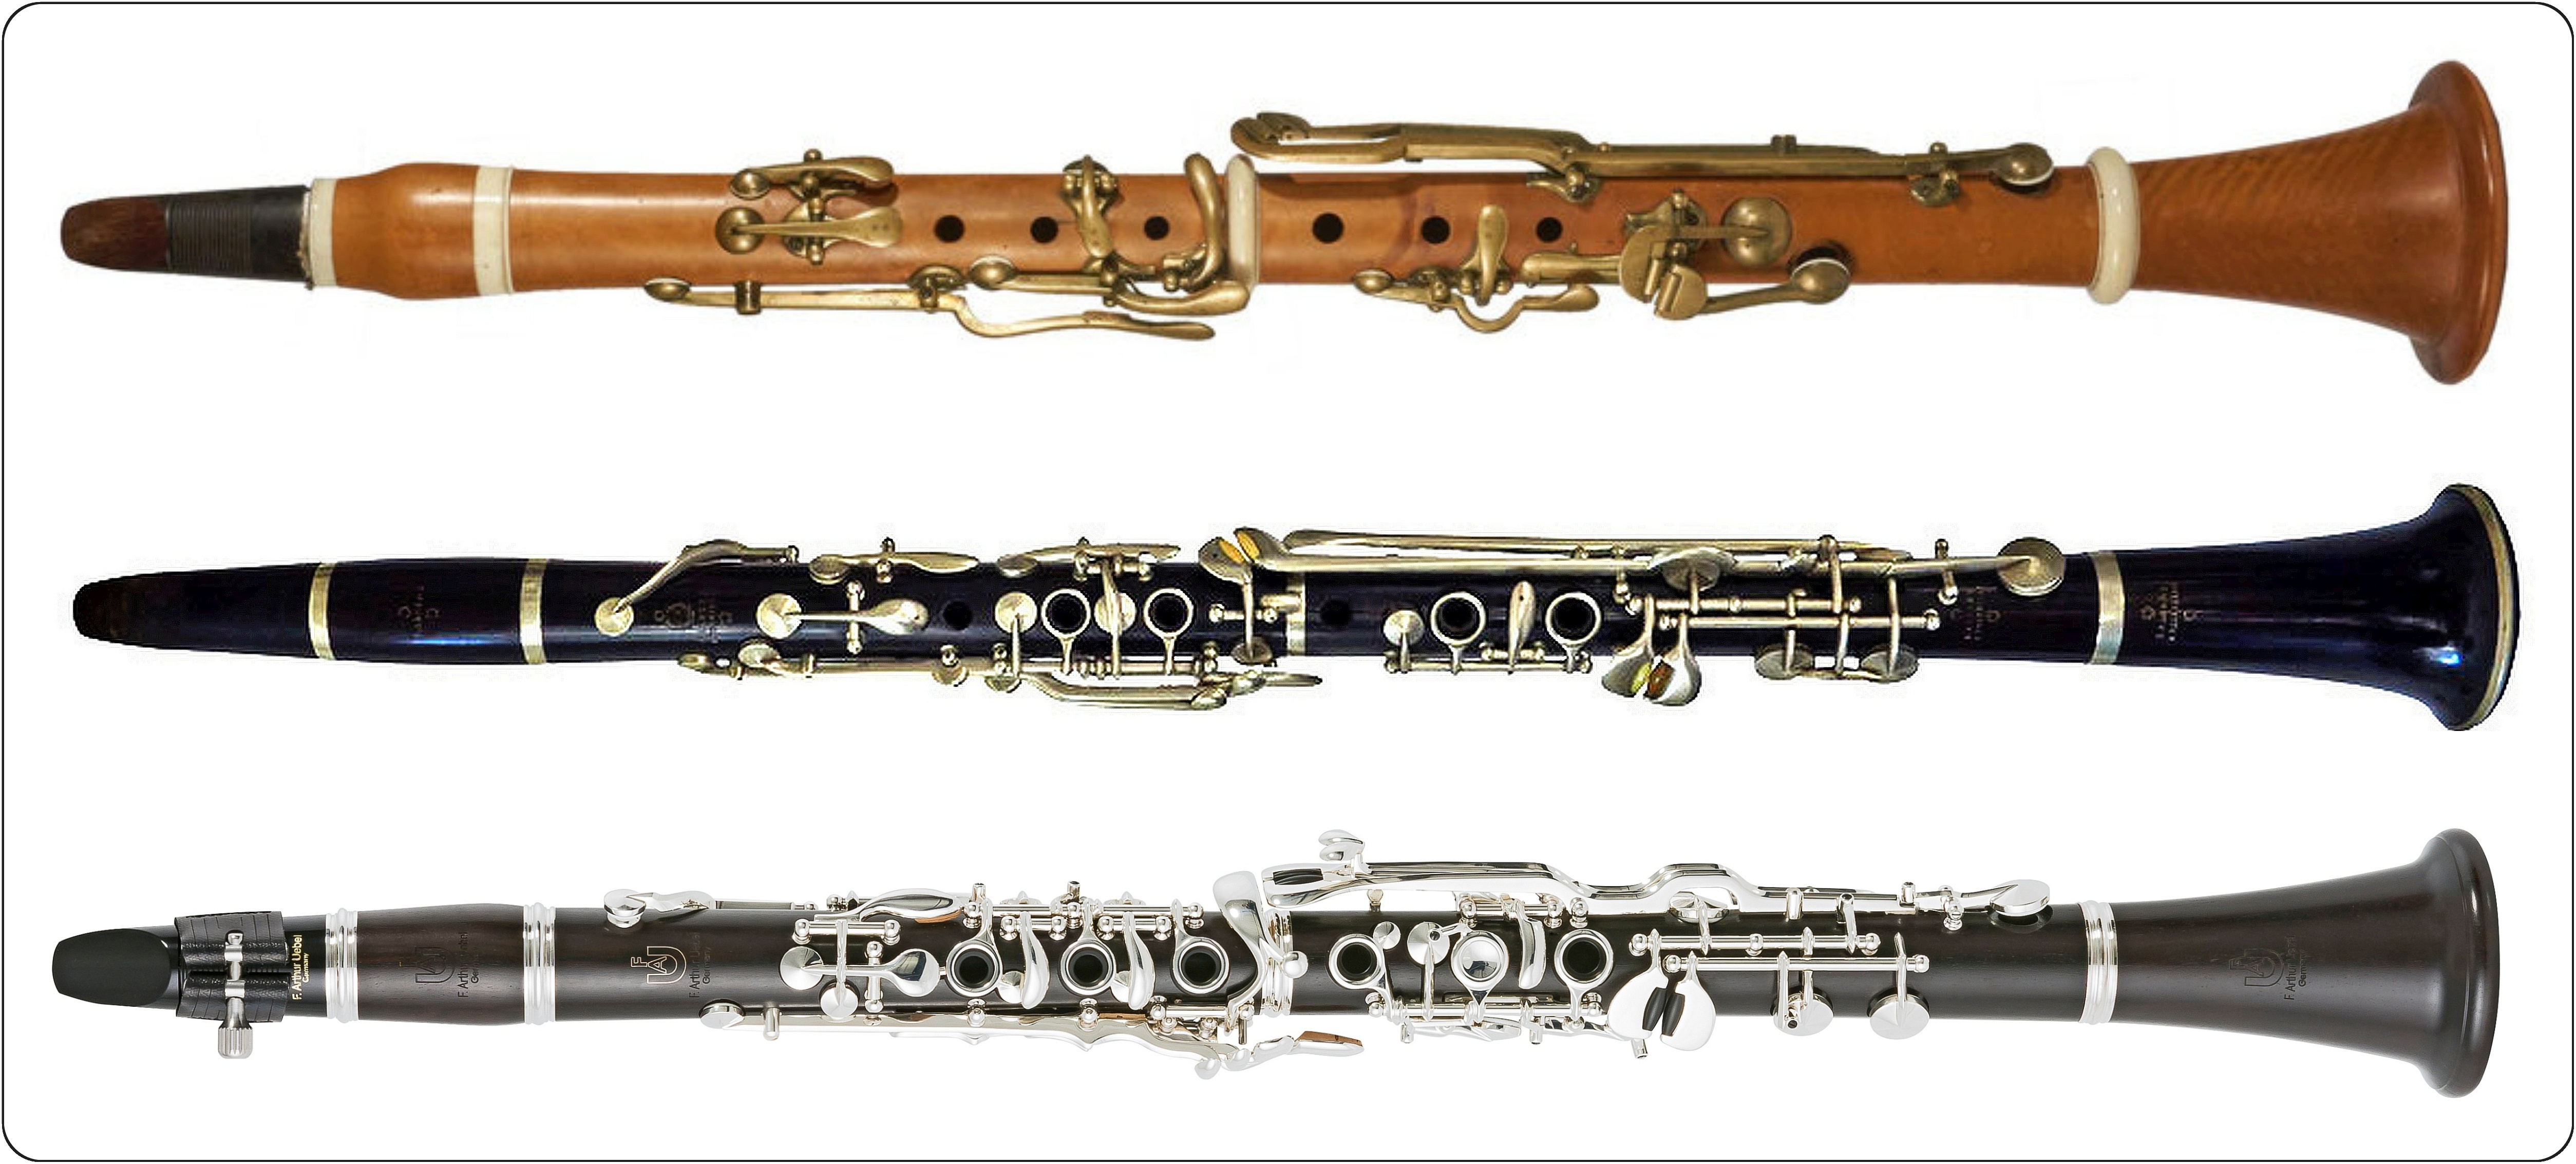
\includegraphics[scale=0.07]{diagrams/M-A-O-clarinets.jpg}
    \caption{A selection of clarinets showing differing levels of key development}
    \label{fig:clKeys}
\end{figure}

The third and final augmentation discussed in this section came into development right at the end of the 19th century: the player piano. The player piano is a wonderful example of the idea of taking an acoustic instrument and enhancing its natural capabilities through additional mechanical or electronic components. This idea of augmented instruments began to grow as the components and technology capabilities increased in power while decreasing in price. The majority of the remaining instruments discussed in this chapter follow this same concept as shown in the player piano.

\begin{figure}
    \centering
    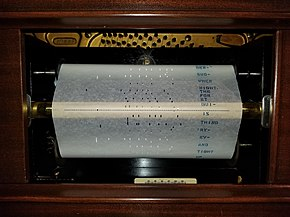
\includegraphics[scale=0.8]{diagrams/PlayerPianoRoll.jpg}
    \caption{A player piano roll}
    \label{fig:pianoroll}
\end{figure}

The player piano functions primarily as a traditional piano. There are no alterations made to the timbre or the action of playing the instrument. However, additional features have been added to the player piano compared to a completely acoustic one. Player pianos started out being able to be controlled through the use of a large spool of paper, called a roll. Holes punched into this paper would be used to manually trigger levers to actuate the piano's hammer mechanisms and generate sound. Early versions of these instruments were operated with a manual pneumatic pump, operated with the feet. Throughout the 20th century, improvements were made to this mechanism including its electrification and eventual digitization. However despite the various technological improvements, a large portion of the market of player pianos is for historic and restored instruments.

\subsection{20th Century Augmented Instruments}
During the 20th century is when a large number of augmented instruments begin to be developed. This is due in no small part to the development of audio amplification and recording during the late 19th and early 20th centuries. One example of an augmented instrument from the early 20th century was the Electric Guitar, which was developed in the 1930's by adding electronic pickups to acoustic guitars\cite{electric_guit_history}.

Following a similar logic as the brass mutes mentioned previously, a prepared piano can be viewed as a kind of augmentation for a traditional piano. The creation of the prepared piano is attributed to John Cage in his 1938-40 composition \textit{Bacchanale}. While more complex and involved than a brass mute, the same concepts apply to the prepared piano. A performer is able to augment the timbral capabilities of the original instrument, the augmentation can be reversed, and the instrument still retains its identity as a piano while prepared. Because of how long it takes to properly augment a piano however, it is less flexible in a performance setting than other augmented instruments. 

\begin{figure}
    \centering
    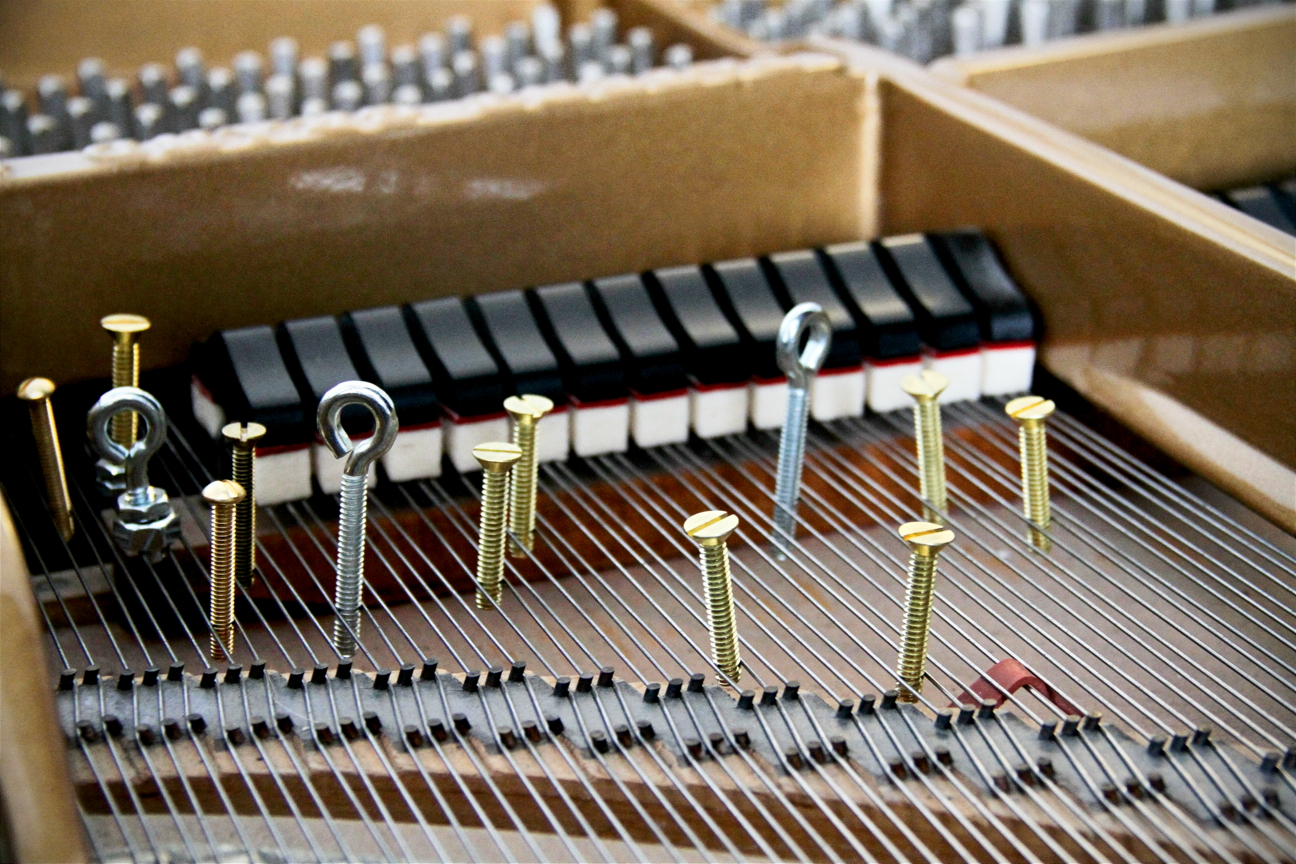
\includegraphics[scale=0.2]{diagrams/IMG_9734_1.jpg}
    \caption{An example of a prepared piano}
    \label{fig:pp}
\end{figure}

The process of preparing a piano is a relatively simple one, if not time consuming. The most common of preparations involve placing small objects on in wedged in between the strings for certain notes. Many composers will\footnote{and should!} include a legend indication how to properly prepare the piano for the performance. These instructions usually include the specific strings, the item/material to utilize, and where/how to place it along the length of the string. Figure \ref{fig:siPrep} shows a page of preparation instructions made by John Cage for his work \textit{sonatas ans Interludes} (1946-48).


\begin{figure}
    \centering
    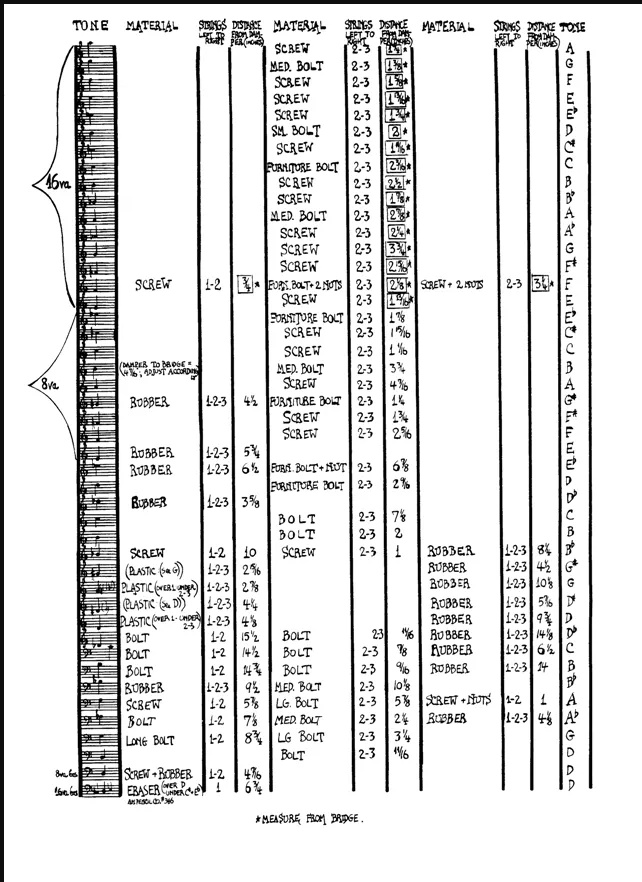
\includegraphics[scale=0.6]{Scores/image_2023-05-08_184813894.png}
    \caption{A page of piano preperations from Cage's \textit{Sonatas and Interludes}}
    \label{fig:siPrep}
\end{figure}

Following the development of computers during the mid-late 20th century, an increase in augmented instruments began to appear during the 1970's on-wards. One example of the instruments developed in this time is the digital sampler. These instruments function similarly to pianos and synthesizers, utilizing the same performance mechanisms. However, when compared to those instruments, the sampler is able to have a much larger range of potential sounds. A sampler records a sample of audio, which can be anything, and re-pitches it along a keyboard range. Many samplers would also include the ability to edit samples and create sequences with them.

\begin{figure}
    \centering
    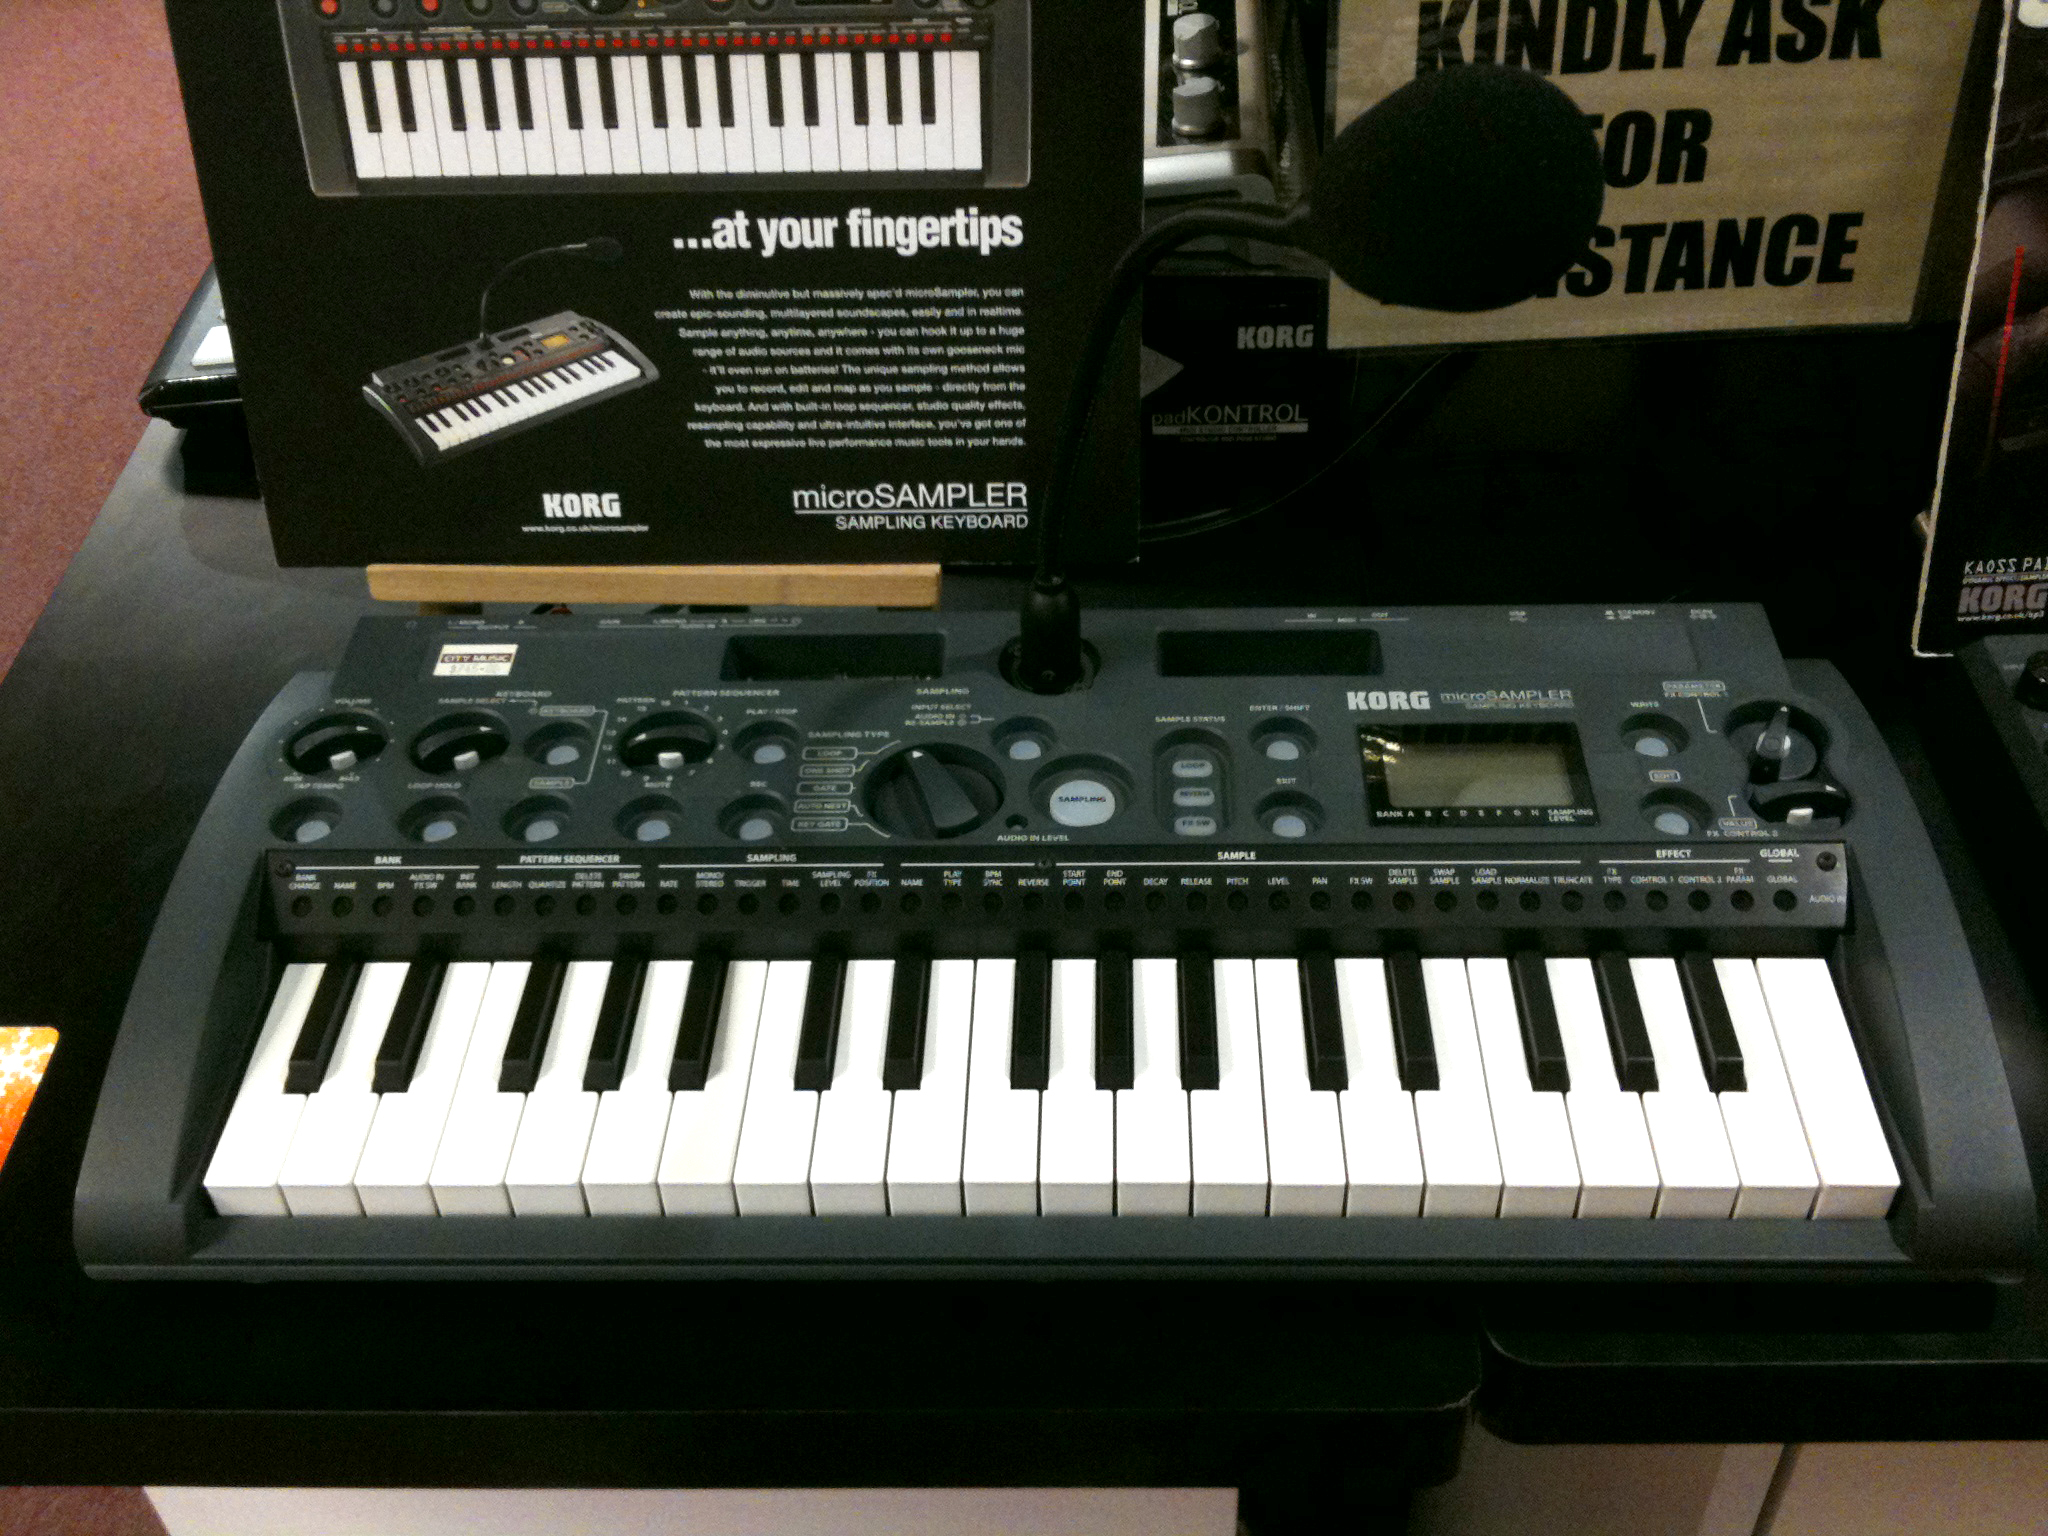
\includegraphics[scale=0.2]{diagrams/Korg_microSAMPLER.jpg}
    \caption{a new Korg microSAMPLER with a keyboard interface.}
    \label{fig:microSampler}
\end{figure}

The Akai MPC was a digital sampler that took a slightly different route than a keyboard interface sampler. Many samplers have a drum pad interface like shown in figure \ref{fig:mpc}. With instruments like these, most of the edits and re-pitching of samples is done prior to a performance or recording. The performer is able to store a large variety of samples and trigger them using the drum pads, which naturally led to its usage in music utilizing strong beats and percussive elements. 

\begin{figure}
    \centering
    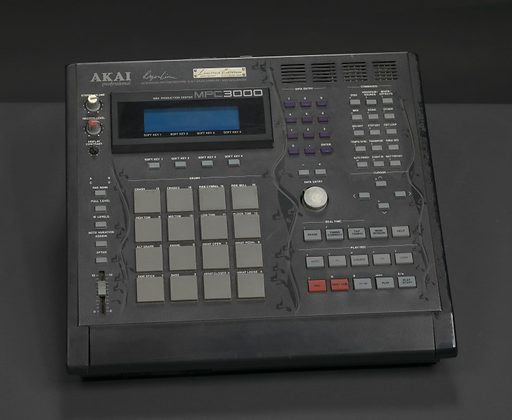
\includegraphics[scale=0.6]{diagrams/YSH000914_MIDI-Production-Center-3000-Limited-Edition-used-by-J-Dilla.jpg}
    \caption{A (fairly dusty) Akai MPC}
    \label{fig:mpc}
\end{figure}

\subsection{21st Century Augmented Instruments}
The difference between 20th and 21st century augmented instruments is ambiguous at best. Electrical augmentation is still prevalent in the practice, but as the components become smaller and more affordable, a further increase in the number of instruments can be seen. %site this claim
Likewise, as computers increased in power, their usage to both locally and remotely control computer augmentation has also increased. This section will look at three specific augmented instruments created in the 21st century with similar design concepts to the Cyberinet.

\subsubsection{MIGSI}

The Minimally Invasive Gesture Sensing Interface, or MIGSI Trumpet is an augmented instrument designed to work with the ergonomics and performance practice of the traditional trumpet\cite{reid2016}. Towards this goal, creator Sarah Belle Reid developed a collection of sensors that fit seamlessly into the form factor of the trumpet. These sensors work to capture control data such as valve placement, hand tension, instrument position, etc. and send it wirelessly to a computer.

All of the instruments discussed here function in a similar way, collecting data and transmitting to a computer to be utilized in some process. In the case of MIGSI, Reid has developed a platform in the Max programming environment which takes the data and parses it out for use within the program\cite{reid_2019}. Reid, has created several improvisations utilizing MIGSI, and written several compositions such as \textit{Consider (2017}) and \textit{Pocket Fig (2015)}.

\begin{figure}
    \centering
    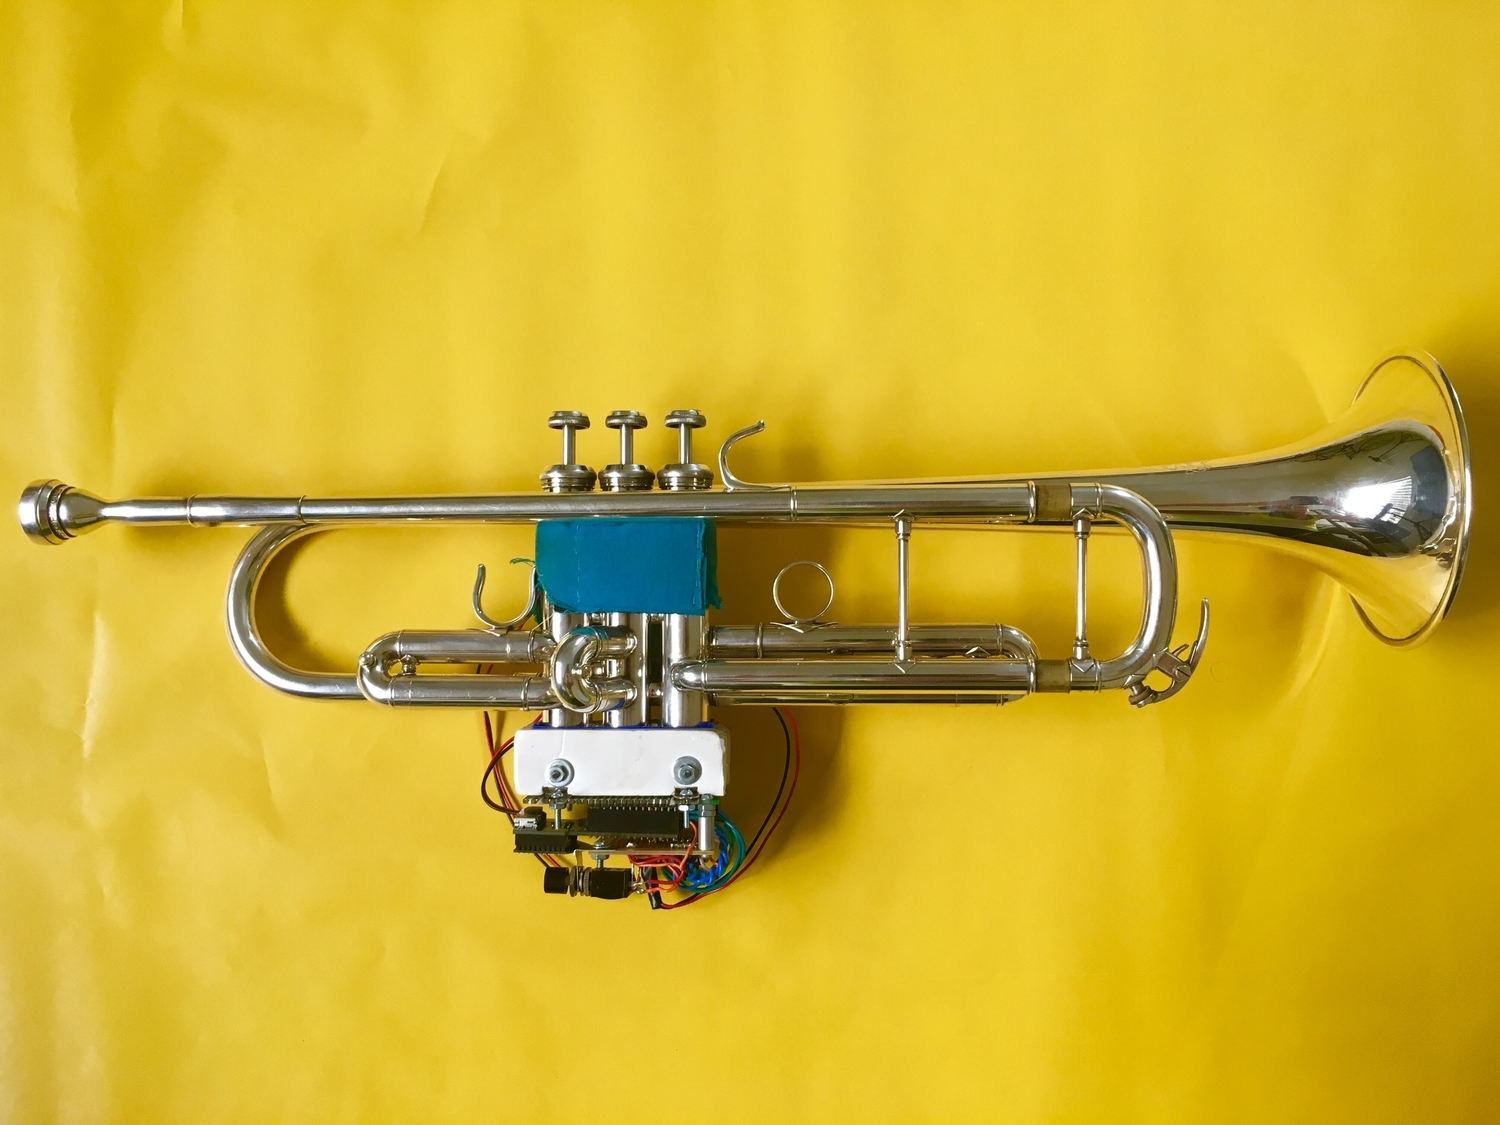
\includegraphics[scale=0.25]{diagrams/MIGSI.jpg}
    \caption{Photo of the MIGSI trumpet from sarahbellereid.com/migsi}
    \label{fig:MIGSI}
\end{figure}


Here we will discuss \textit{Pocket Fig} for the MIGSI Trumpet, written by Sarah Belle Reid\footnote{A performance video of \textit{Pocket Fig} can be found at \url{https://www.youtube.com/watch?v=5szWkbVjYxg}}. In this improvisatory work, Reid utilizes Force Sensitive Resistors as well as Infrared sensors to collect data related to the valve displacement on the instrument. This data is then wirelessly sent to the computer to control a Max patch's granular synthesis processing. The end result is, in Reid's own words: 

\begin{quote}
    "a flurry of classic computer music sounds, stutters, and granular synthesis gestures based on the voice and trumpet sounds of the performer."
\end{quote}

This flurry of effects are heard in performances as soon as the performer begins either significant movement, or begins to press the trumpet valves. In this particular composition, the performer is recorder with a microphone and also able to utilize their positioning around it to change the resulting sounds.

% Where the MIGSI is similar to the Cyberinet is in its goals of form factor. The entirety of the MIGSI augmentations are located to match the form of a standard B-flat or C trumpet, and is placed at the instrument's center of gravity to minimize fatigue from the extra weight. While not as streamlined as the MIGSI trumpet, the Cyberinet's sensors are located in a similar location in relation to the design of the Clarinet.


\subsubsection{SABRe}

The SABRe is another sensor array that is designed to work with various woodwinds, opposed to the trumpet MIGSI is compatible with. The unit straps onto the instrument and can be used to collect airflow and position data to be wirelessly sent to a control computer. While effective and easily removable, this particular device offers a relatively limited amount of usable parameters which can be utilized in an augmented instrument. In the majority of cases this is not problematic, as like the MIGSI, the choice in sensors matches with the common performance gestures of the instruments using it.\footnote{We will see modularity in physical design come into play with the Cyberinet.}

Similar to MIGSI, SABRe is intended to also be minimally invasive to the performer. It is intended for use mainly with clarinets, being originally prototyped on a bass clarinet, but can be easily applied to many single-reed instruments\cite{Schiesser2012}. The goal of the SABRe is to provide augmentation features to performers, regardless of their technical abilities\cite{Schiesser2012}.

SABRe utilizes four main sensors as well as an additional set of buttons that can wirelessly communicate with the main unit. These include gyroscopic and accelerometer data, airflow sensors, and buttons.\footnote{There are a few more sensors in the SABRe, but the ones mentioned are the main ones advertised.}

\begin{figure}
    \centering
    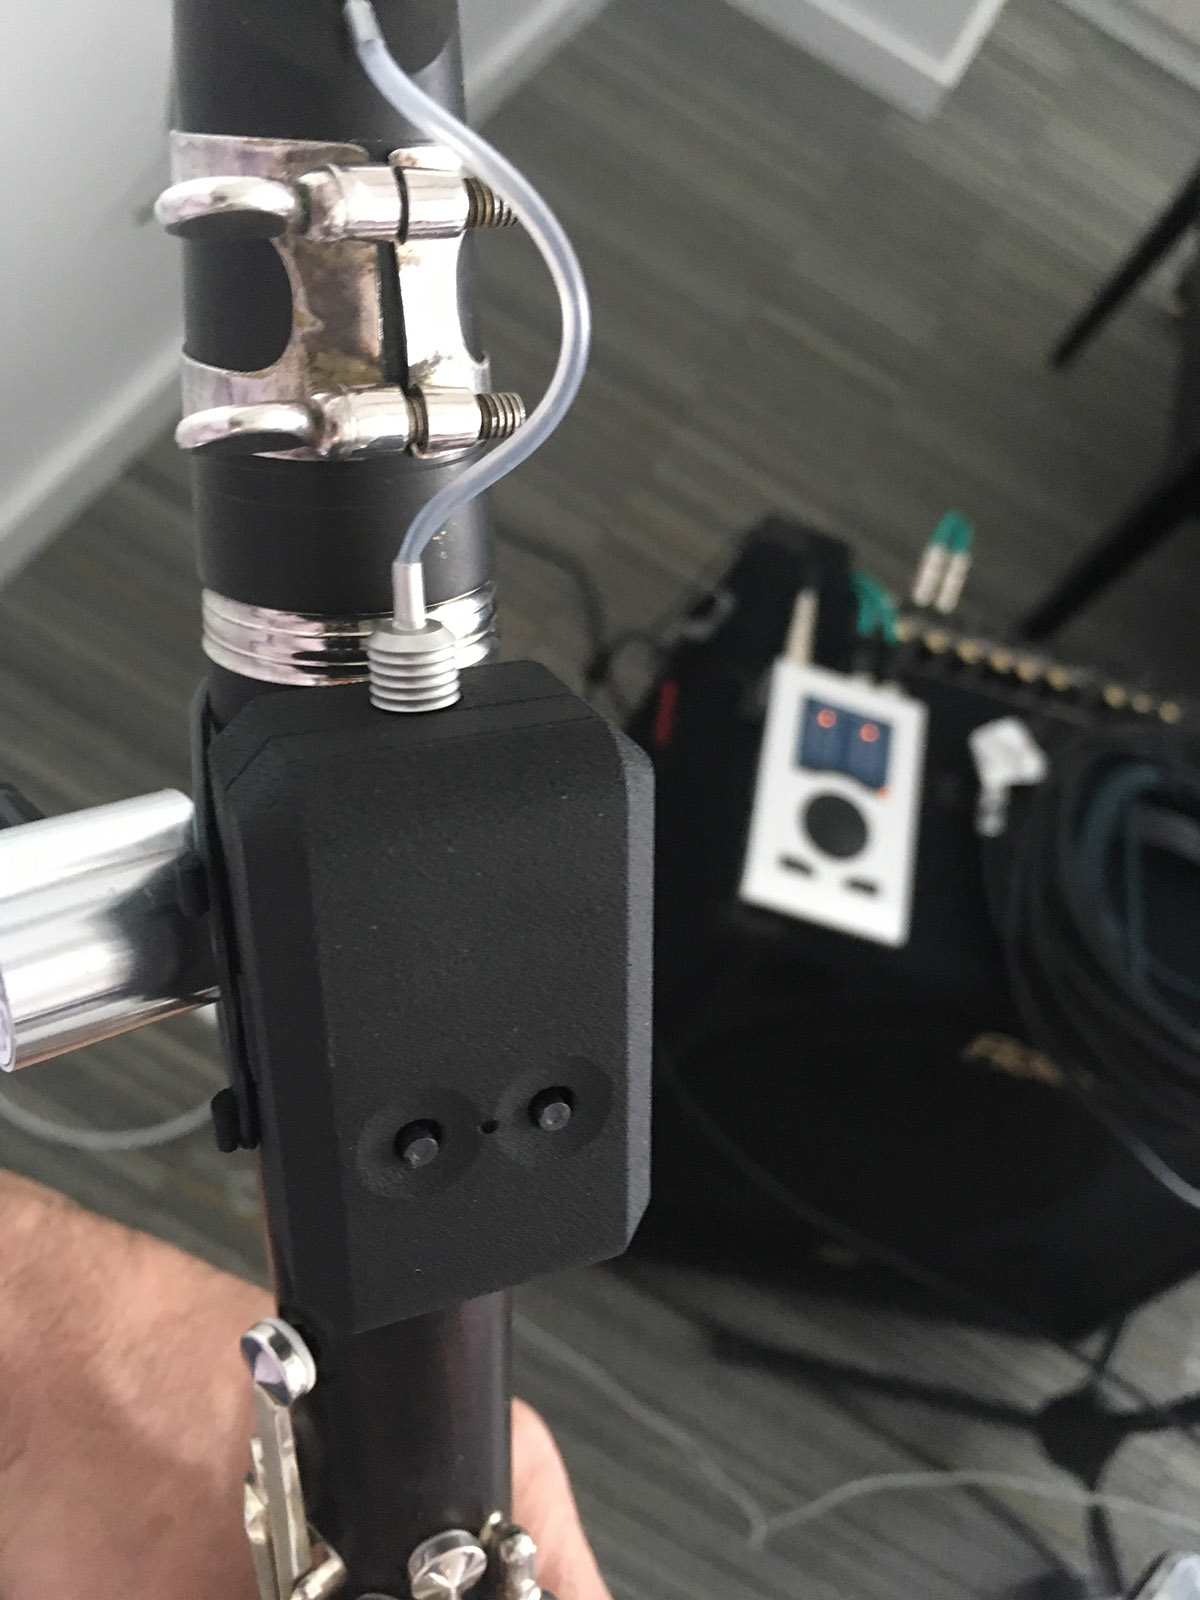
\includegraphics[scale=0.2]{diagrams/sabre-right-hand.jpg}
    \caption{SABRe on a clarinet}
    \label{fig:SABRe}
\end{figure}

Prior to 2023, SABRe had been on a hiatus in terms of development and is currently in the process of designing a relaunch of the system. It is perhaps for this reason that there is a limited number of works for the system, but discussing the reasons behind the hiatus is beyond the scope of this paper. Unfortunately however, the majority of resources provided by SABRe online have been taken down pending their eventual relaunch of the system. Differences may occur between the original version and the second iteration. The original one utilized a software program developed by SABRe to control the receiving and control of the data for audio processing. 

% As well as containing a similar base, the units also allow for an optional use of 2 buttons that can be programmed using the computer. However, it is at this point that the sensors begin to differ. It is the view of the author that the SABRe sensor is generally lacking in two main elements. The first is its lack of additional sensor options. While the included sensors are indeed quite useful for collecting performance data.


One piece that will be discussed is  \textit{Sailing}\footnote{The performance of \textit{Sailing} can be found at \url{https://www.youtube.com/watch?v=Eiuacb5nJc8}} by the SABRe's creator: Matthias Mueller.  

In this work, Mueller takes the gyroscopic information from the SABRe to control audio effects in real time. The first one heard is the control of the amount reverb and delay time as the performer moves from right to left. This is followed by triggering a tremolo effect that combines with the clarinet timbre. Due to a lack of a score, it is my best guess from the video that this effect is being toggled on with the buttons located on the back of the instrument. By combing these effects with micro-tonal notes, Mueller is able to create a unique sound world easily and effectively.

Mueller also utilizes a pitch shifting effect, but it is unclear if it is created as a unique harmonizing effect, or is created as a byproduct of adjusting delay times. The final effect is a little distortion present when the performer reaches the extreme ends of the gyroscopic data.

In the future, should a performance score become available, it would warrant more in depth analysis of the performance practice and specific utilization of the SABRe's sensors. However, there is still much that can be learned with Mueller's performance video. It can be seen that Mueller clearly focusing on only one or two sensors present within the SABRe: Gyroscope and Buttons. By focusing on a smaller subset of the sensors, it allows Mueller to allow the capabilities to the system to stand out. It becomes very clear what the correlation between the clarinetist's physical position and the timbres being created are.

Mueller's utilization of the button is worth bringing up individually. in \textit{Sailing}, Mueller is using this button to trigger a tremolo-like effect to be applied to the clarinet's signal. Unfortunately without the software patch or score the fine details of this are left to speculation, but I want to focus on the idea of manually triggering an effect with a button. Unlike a foot pedal, these buttons follow the performer, allowing them to take full advantage of the buttons along with the movement sensors. A performer can access the buttons regardless of their on-stage location.

% As well as containing a similar base, the units also allow for an optional use of 2 buttons that can be programmed using the computer. However, it is at this point that the sensors begin to differ. It is the view of the author that the SABRe sensor is generally lacking in two main elements. The first is its lack of additional sensor options. While the included sensors are indeed quite useful for collecting performance data.

\subsubsection{Hyper-Flute}

There are many more augmented instruments that have been developed in the 21st century so far. A full study of them would warrant an entire other dissertation.\footnote{A few other examples include the Meta-Sax, Overtone Violin, Haptic Drums, the instruments discussed by Reid et al\cite{reid2018}, and instruments developed by the Augmented Instruments Laboratory in London.} We will wrap up our discussion of recent augmented instruments with the Hyper-Flute.

\begin{figure}
    \centering
    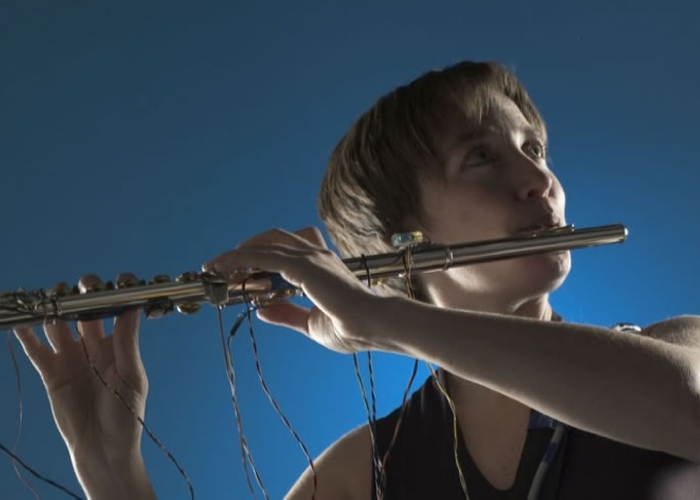
\includegraphics[scale=0.5]{diagrams/palacio_quintin_cleo.jpg}
    \caption{Cléo Palacio-Quintin performing on the Hyper-Flute}
    \label{fig:hyper-flute}
\end{figure}

Developed in 2003 by flutist/improviser/composer Cléo Palacio-Quintin, the Hyper-Flute is a Powell 2100 model flute with a handful of sensors embedded into various locations along the instrument. \cite{hyper-flute2003}. Palacio-Quintin's stated goals in developing the instrument are: 

\begin{quote}
    ...[preserve] the intimate relationship between my body, my instrument and the sound it produces. I wanted to keep intact the acoustic richness of the flute, and my way of playing it. The computer had to become a virtual extension of the acoustic instrument \cite{hyper-flute2003}.
\end{quote}

Towards this goal, Palacio-Quintin ultimately decided on six unique sensors that can control the computer processing of the flute. While there are some overlaps between the Hyper-Flute and the other instruments discussed in this chapter, the design implements a variety of unique ideas not present in the other wind instrument augmentations discussed. Firstly is that the Hyper-Flute is not a removable augmentation like SABRe or MIGSI. These sensors, listed in figure \ref{fig:hyper-flute-sensors} are permanently installed onto the flute. 


Voltages from each of these analog sensors are then analyzed and converted to a MIDI value which can be sent to a computer or MIDI compliant instrument. All of the data is sent as  continuous control MIDI messages. What I find particularly interesting about the Hyper-Flute is that while Palacio-Quintin has developed various software patches using Max, similarly to the other instruments discussed in this chapter, because the data being generated is MIDI compliant, the Hyper-Flute can easily interface and control a large variety of instruments via the MIDI port, which can open an entirely different world of performance practice and possibilities when compared to other instruments\cite{hyper-flute2003}.

\begin{figure}
    \centering
    \begin{enumerate}
        \item Magnetic field sensors to detect pinkie-key movement.
        \item Ultrasonic distance sensor to detect distance from the computer.
        \item Tilt switches to detect movement and rotation of the instrument.
        \item Pressure sensors located where the performer holds the instrument.
        \item Light sensor to detect ambient lighting changes.
        \item Button switches which can be activated by the thumbs while performing.
    \end{enumerate}
    \caption{Sensors present in the Hyper-Flute.}
    \label{fig:hyper-flute-sensors}
\end{figure}

In musical performance, the use of sensors can be seen in Souffles Électriques, a small collection of various works for the Hyper-Flute.\footnote{Souffles Électriques can be found online at\url{https://vimeo.com/155153474}.} While not discussed in the original 2003 paper, Palacio-Quintin has since expanded the range of instruments to include at least the Bass Flute as well as the original Concert Flute. The performer is able to intuitively control the sounds from the various sensors. Effects such as adjusting audio processing and the playback of samples by pivoting the flute angles and position in three dimensions are seen in the performance, as well as the use of the magnetic field sensors in the pinkie keys.


\section{Cybernetics}
In addition to being an augmented instrument, the Cyberinet utilizes cybernetic principles in its design and intended uses. To better understand this connection, let us look into the concepts of Cybernetics and Cybernetic music.

\subsection{General Cybernetic Concepts}
The concept of modern cybernetics was defined by Norbert Wiener in his 1948 book \textit{Cybernetics: Or Control and Communication in the Animal and the Machine}, which has been republished by MIT press in recent years\cite{WeinerCybernetics2019}. The republished versions contain additional supplementary chapters not included in the original 1948 publication.

%finish book and verify that this is indeed the correct first definition.
In its original context, Cybernetics is defined as \textit{The science of communications and automatic control systems in both machines and living things}. While the concepts of cybernetics were present before Wiener, it was in his writings that the term Cybernetic were formally created. Wiener credits J.C. Maxwell in his 1868 paper as one of the first formal studies into what would ultimately evolve into Cybernetics. In that paper, Maxwell discusses the concept of a Governor and moderator within a variety of mechanical system\cite{maxwellOnGoverners}. Wiener posits that perhaps one of the earliest examples of the work as described by Maxwell is that of the steering mechanism of a boat\cite{WeinerCybernetics2019}. Heavily summarized, this is the idea that a sailor can see and respond to the conditions they are sailing in by turning the wheel, which, through mechanical means described by Maxwell, causes the boat to turn, thus altering its condition.


As time progressed, the definition of cybernetics has evolved. Scientifically, the definition is relatively unchanged, still focusing on feedback systems and automated responses, but now also refers to the combination of mechanical an organic components to help achieve this. %citation needed

For example, take the Omnipod 5 system used for diabetics to manage their insulin delivery. This device has the capability to be paired with a constant glucose monitor embedded within the user's abdomen. This sensor will read the glucose levels of the user and automatically adjust the Omnipod 5's insulin delivery rate to compensate for any changes to the blood glucose levels. This system is cybernetic in every sense of the word. It both combines organic and inorganic components, as well as the internal feedback loops to control the blood glucose level of a diabetic in a manner similar to a person without diabetes.

\begin{figure}
    \centering
    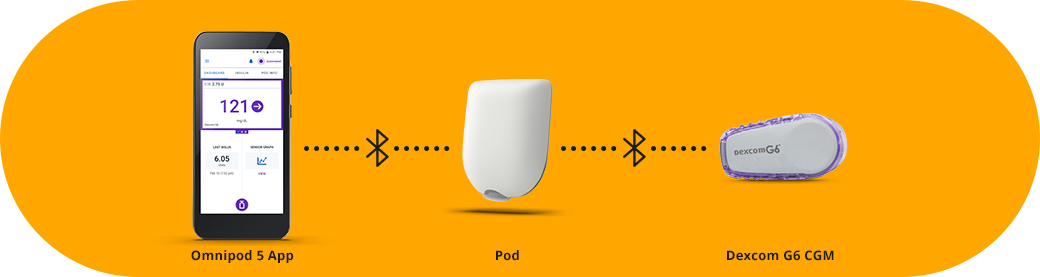
\includegraphics[scale=0.4]{diagrams/Omnipod-5_CGM_Pod_BT_1040x277.jpg}
    \caption{Diagram made by Omnipod showing the communication of the Omnipod 5.}
    \label{fig:my_label}
\end{figure}

The focus on combining organic and inorganic components comes in no small part from popular culture. Cyborgs were first introduced in science fiction during the middle o the 19th century and have become a major part of the entertainment industry since then. the word cyborg is a portmanteau of cybernetic and organism, and serves to show the melding of organic and inorganic components to form a new being.

Another cybernetic concept present in music composition of the 20th century is that of second-order cybernetics. The core differences between first and second order cybernetics is the inclusion of the observer within the cybernetic system. Rather than a completely isolated system, a person in a second-order cybernetic system is able to observe and react, altering the system and controlling the output to various degrees. In terms of musical composition, this allows for a composer to both allow for the unique characteristics of cybernetic systems, but still control the output enough to give the final result their own unique flair.



\subsection{Cybernetic Music Practices}
As previously mentioned, cybernetic principals have also been utilized in music composition. Various composers have utilized cybernetic ideas to create music that can evolve over time. These effects can give the music a unique character and identity. Implementing cybernetic music can happen through both entirely acoustic means, as well as through computer controlled algorithms.



\subsubsection{Herbert Brün \textit{(1918-2000)}}
Brün was both a composer and computer scientist who focused on cybernetic concepts in his various works. Many of these works were programmed in early coding languages such as FORTRAN which allowed Brün to incorporate both randomness and Cybernetic feedback into the music generation process. In a handful of works, such as \textit{mutatis mutandis} from 1968, would utilize random number seeds in order to create visuals which were then interpreted by musicians.

In relation to Cybernetics, Brün was influential in the development of Second-Order Cybernetics along with other scientists such as Heinz Von Forester and Margaret Mead. Second-Order Cybernetics ultimately developed into a process which is heavily utilized in Cybernetic music moving forward. In short, the main feature of Second-Order Cybernetics is the inclusion of the observer in the Cybernetic system, as opposed to them existing outside of it\cite{Scott_2nd_order_Cyber}. In relation to the creation of music, this meant that a composer utilizing this concept would be able to create a cybernetic system, and then directly influence it in order to affect the outcome.


\subsubsection{Roland Kayn \textit{(1933-2011)}}
A German born composer who was heavily inspired by information sciences when creating his unique style of mainly electronic and electroacoustic music\cite{rolandKaynBio}. His earliest works to utilize the cybernetic concepts was \textit{Galaxis} (1962) for a variable acoustic instrumental ensemble and \textit{Cybernetic} (1969) for electronics. Kayn would write several more over the following years. These works incorporated cybernetic principals in what Kayn referred to as being "self-governing"\cite{rolandKaynBio} and "able to think for itself\cite{Kayn_Elektroakustische_Projekte}. In the context of Kayn's electronic music, this was present in algorithmic processes which incorporated semi-random calculations. These unpredictable results were then fed back into the system which resulted in unpredictable, autonomous results\cite{rolandKaynBio}.

\begin{figure}
    \centering
    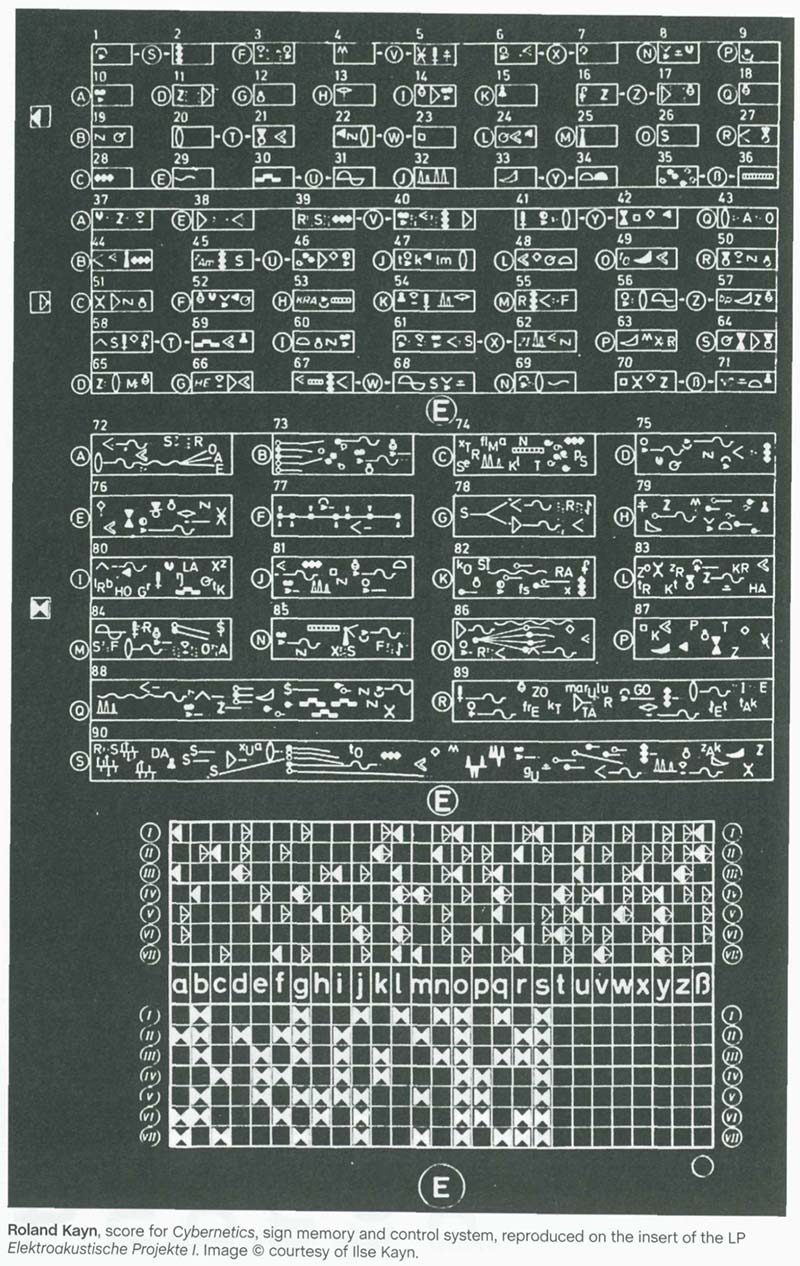
\includegraphics[scale=0.45]{diagrams/kayn_cybernetics.jpeg}
    \caption{\textit{Cybernetics I} (1969) score}
    \label{cyberneticsScore}
\end{figure}


% show randomsness in the score to make point.
Figure \ref{cyberneticsScore} shows one of Kayn's works, \textit{Cybernetics I} from 1969, and shows the various electronic components used to generate the sound in the top portion, and how those components interact in the bottom portion, similar to the matrices used in synthesizers of the era. Looking at the score, we can see how the output of certain processes are fed back into the system, causing the feedback loops common to Cybernetic music.


\subsubsection{Pauline Oliveros \textit{1932-2016}}
An American composer, performer, and educator. Oliveros was a founder of the San Francisco Tape Music Center and pioneer of Deep Listening\cite{HolmesElectronicMusic2020}. Deep Listening is a school of thought at method of listening described by Oliveros as:

\begin{quote}
    ... For me [Oliveros], Deep Listening is a lifelong practice. The more I listen the more I learn to listen. Deep Listening involves going below the surface of what is heard, expanding the whole field of sound while finding focus. This is the way to Connect with the acoustic environment, all that inhabits it , and all there it.

    For others, Deep Listening is a practice consisting of listening and sounding exercises and pieces I and others have composed since 1970. The results are proceeded by a group of discussions in workshops and retreats. 

    Deep Listening is for musicians as well as participants from other disciplines and interests. Previous musical training is not required\cite{cultureandHumanity2002}.
\end{quote}

In short, the idea of Deep Listening itself is a cybernetic practice\cite{gordosOliverosCybernetics}. This is because of Deep Listening's core principle of listening to how you listen. The act of a system responding to itself in a feedback loop is a core concept in cybernetics. In relation to Olivero's music, the concepts of deep listening and cybernetics can be clearly seen in her tape improvisations of the 1950's and 60's. In these works Oliveros along with a variety of collaborators would record themselves improvising, then listen to the recording and discuss what they heard. Following this the group would repeat the process until they were pleased with the results\cite{gordosOliverosCybernetics}. 

\begin{figure}
    \centering
    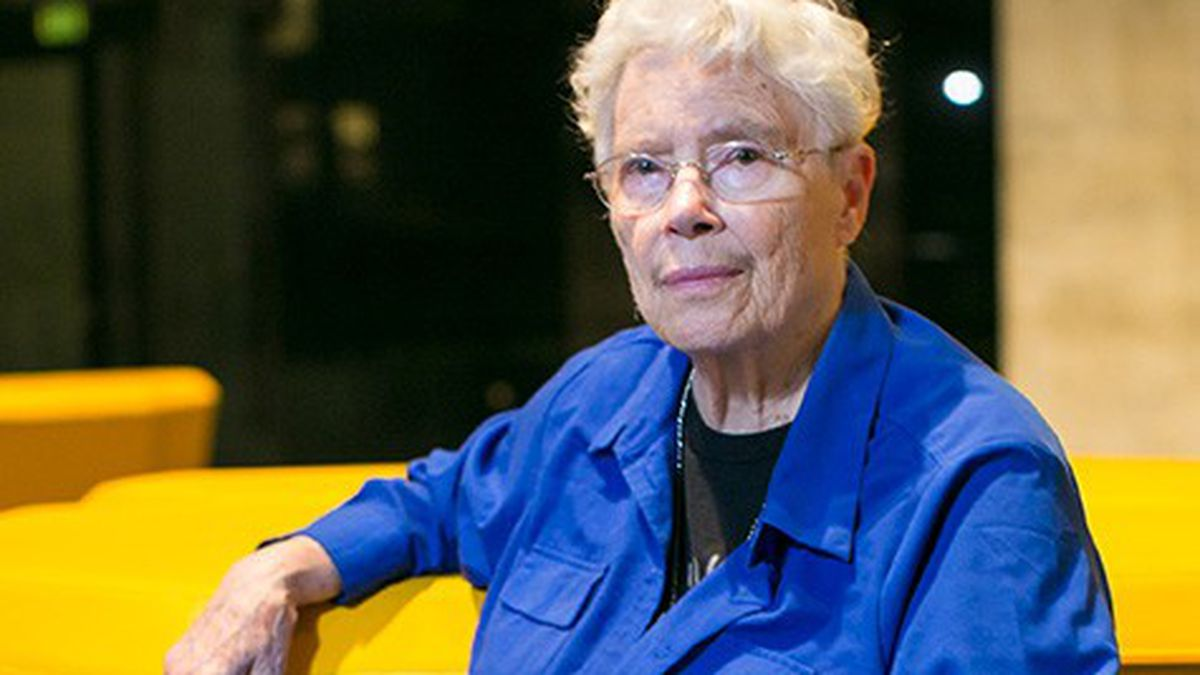
\includegraphics[scale=0.25]{diagrams/oliveros.jpg}
    \caption{Pauline Oliveros}
    \label{fig:oliverosHS}
\end{figure}

Another series of works with cybernetic principles is Olivero's \textit{Sonic Meditation}s (1974). \textit{Sonic Meditations} is a collection of 25 different actions intended to cause the performer to intensely focus on their action, the sounds around them, and the sounds of their actions\cite{OliverosMeditations}. The instructions are all given as text have been performed in a traditional setting or individually, but in the score Oliveros intends to remove nay connotation of traditional performance and focus on the sound through \textit{Deep Listening.} 

These prompts range in complexity and specificity ranging from talking a walk with as quiet of steps as possible to singing pitches in groups until a single pitch is established. There are also more complex activities focused on breathing and the acts of making, listening to, imagining, and remembering sounds\cite{OliverosMeditations}. By actively guiding the performer through the \textit{Deep Listening} activities, all of the cybernetic principles of \textit{Deep Listening} become present in the music performance as well. All 25 pieces have in some way the performer listening to a sound occurrence and responding by altering their actions to change the sound environment.

\section{Defining the Cyberinet}


Taking the last several pages into account, let us begin to define exactly what the Cyberinet is, and the main goals it works to achieve. First and foremost, the Cyberinet is an augmented instrument designed to bring a cybernetic level of control to the Bb clarinet. When comparing it to the three aforementioned instruments, there are several features that the Cyberinet iterates on, and several that it does not embody.

In relation to MIGSI, The Cyberinet is designed to be minimally invasive. While a performer can interact with the instrument in novel ways to create interesting effects through the sensors, utilizing MIGSI and the Cyberinet by itself should not impede the traditional performance practice of the performer. % negatives of the MIGSI here

The Hyper-Flute is able to interact with a variety of devices using a MIDI port. While not identical, the Cyberinet software is intended to be able to interact with a variety of hardware and software using Max as the main platform. However, the large number of wires hanging from the Hyper-Flute are both distracting in a performance setting, and can potentially obstruct the performer's movement\footnote{A portion of this drawback is due to the development of more powerful and smaller digital sensors in the 20 years between the development of the Hyper-Flute and the Cyberinet}. The Cyberinet wirelessly communicates with the computer with only external wires needed to connect to optional expansion sensors or to charge the Cyberinet.


Of the discussed instruments, the SABRe is a system of sensors that is the device most closely related to the Cyberinet. This is in no small part due to the fact that they are designed to augment the same instrument. Specifically comparing the two devices, we can see clear pros and cons to both SABRe and the Cyberinet, shown in figure \ref{fig:proCon_SABRe_Cyberinet}.

\begin{figure}
    \centering
   \textbf{SABRe:}

\begin{itemize}
    \item Pros: small, completely wireless, easily removable.
    \item Cons: no modularity, cost.
\end{itemize}

\textbf{Cyberinet:} 

\begin{itemize}
    \item Pros: integrated within the instrument, expandable with add-ons, relatively inexpensive to produce, open source-components.
    \item Cons: less easily removable, some wires involved.
\end{itemize}
    \caption{Pros and Cons of the SABRe vs the Cyberinet}
    \label{fig:proCon_SABRe_Cyberinet}
\end{figure}

When utilizing the SABRe, I felt that while extremely simple to set up and utilize, the lack of additional sensors could hamper potential uses. The chosen sensors, listed in the following chapter are all useful in collecting clarinet performance data, but it cannot be customized outside of adding two buttons to the system. To help avoid this potential limitation in the Cyberinet, the Cyberinet is designed to be able to attach an expansion unit with an additional sensor\footnote{This was also done in order to help differentiate the Cyberinet from the SABRe in terms of design and functionality.}. These sensors are discussed more in Chapter 2, but are all compatible with OEM components and utilize the same voltage ranges. This allows them to be hot-stoppable in a performance setting.

The final aspect of the SABRe that the Cyberinet intentionally differs from, other than physical design, is the cost. The initial version of the Cyberinet is designed to be completely open-source, utilizing OEM components. While this does increase the overall size of the Cyberinet, it results in a final unit that is significantly cheaper to manufacture than the SABRe.\footnote{The initial version of the SABRe retailed for approximately €500.} Even with a 100\% markup, the final cost of the Cyberinet, mentioned in Chapter 2, is less than half that of the SABRe. By having a cheaper development cost, it is my goal that more people will be able to utilize the Cyberinet due to a lower cost-of-entry wall. In fact, is a person already has a 3D printer, then they can completely create and program a Cyberinet from scratch for only the cost of the materials.


Van Nort describes Digital Musical Instruments as being either implicit or explicit in regards to their use of the control data. Where explicit designs are analytically described and implicit interactions are applied through some sort of training\cite{vanNortMapping2007}. In his paper, Van Nort goes on to describe a handful of other interactions between the data being collected and the sound being produced. Using the terms defined there, the Cyberinet can be described as using an implicit, dynamic, and continuous use of the performance gestures. Controls are based on clarinet performance practice and not a new set of skills, the sensor types can change through its designed modularity, and the sensor data is continuously being collected while in use. There is also a multiple layers of mapping between the raw data and what is utilized to produce sound. This is to help further draw correlations for gesture recognition as well as ease of use when programming.

Looking back at the instruments discussed previously in this chapter, we can see many of the instruments share similarities with the Cyberinet in this design choice. While none of the aforementioned instruments would be considered dynamic for the same reason as the Cyberinet, they all collect continuous data using implicit means. The Hyper-Flute specifically maps the data to MIDI for use in other devices, while MIGSI and SABRe can have the data further mapped within the Max software. Due to the ability for the mapping to change within the software environment for all four of these instruments, each one is capable of adapting and changing the mappings in real time, an act which Van Nort describes as the mapping becoming playable itself\cite{vanNortMapping2007} in a fashion similar to the idea of Second-Order cybernetics.



Ultimately, the Cyberinet can be defined as a new augmented instrument, which can be implemented with a standard B-flat clarinet. This augmented instrument collects data from various embedded sensors and transmits the data to a nearby computer while the performer plays the instrument traditionally. The sensors can be adjusted in a semi-modular fashion; by adding or removing expansions to the two main ports on the main unit. The Cyberinet is intended to be affordable to produce, using OEM components with open-source resources. This is to allow for more accessibility to a wider range of performers and composers wishing to work in electroacoustic music. Lastly, because of the Cyberinet being able to control audio processing through the act of performing on the clarinet, it brings a level of cybernetic awareness to the performer as well. A performer will be able to perform and hear how their actions are influencing the music and either positively or negatively reinforce that control by adjusting their playing. 

But how exactly will the performer be able to influence their playing? A performer composer or performer could create specific movements at specific times to trigger an effect, this could be pre-planned or improvised. A student could monitor the data while learning the instrument to check their positions and breath control. This is just a short list that will be explored more in Chapter 4. As we will see, the potential for sound and control options are astronomically high, but there are a handful of useful methods and interactions envisioned by the author, which can help guide newcomers to the Cyberinet.



\chapter{Building the Cyberinet}




% At its core, the Cyberinet contains a small collection of sensors build into the hardware. These include: [list of sensor names]. In addition to these sensors, the unit contain two USB-C connectors on its side. The first one is intended for the button board expansion, which gives the performer access to two buttons positioned on the thumb rest of their instrument. The functionality of these buttons can then be programmed using Max or another audio programming environment. The second USB-C port is designed to connect to a variety of other sensors, allowing for the performer to adjust their setup for whatever is needed for a particular performance. This is the origin of the phrase “semi-modular” in the project title. At the time of writing, one expansion sensor has been created and tested. This is the [figure something out, a mic that will respond to volume and transmit a bang.] Additional expansions have been planned and explored in more detail in the “Further Directions” section of this document. 
% All these chips were selected for their ability to be dropped into the main board without an extensive need for the user to solder many components, and their use of standard 0.1 inch spacing. [fix this sentence]



\section{Cyberinet Design Process}


When developing the functionality of the Cyberinet, the steps defined by Miranda and Wanderley in their book\cite{miranda_Wanderley_instrumentControl_2006} helps to organize and streamline to process. Paraphrased, that process is shown in figure \ref{fig:DMIProcess}. This chapter will follow the process given here and breakdown exactly how the Cyberinet was created.

\begin{figure}
    \centering
    \begin{enumerate}
    \item Determine gestures that will control the instrument.
    \item Determine how to capture the gestures for use within the system.
    \item Define the specific sound creation processes that will be controlled by the sensors.
    \item Map the gesture control data to the desired sound-creation parameters.
    \item Decide on the feedback mechanisms for the performer to be able to respond to.
\end{enumerate}
    \caption{Digital Instrument Design steps as defined by Miranda \& Wanderley\cite{miranda_Wanderley_instrumentControl_2006}}.
    \label{fig:DMIProcess}
\end{figure}

\subsection{Control Gestures \& Gesture Sensing}
The main control parameter for the Cyberinet is traditional clarinet performance. This process was ultimately chosen in order to help highlight the intended use cases for the Cyberinet\footnote{See Chapter 4 for more information on intended uses of the Cyberinet.}. All of these seek to enhance the clarinetist's sound capabilities without transforming the Cyberinet into a completely new instrument. At its core, an augmented instrument must still retain its identity as the original instrument\cite{miranda_Wanderley_instrumentControl_2006}. Towards this goal, a breakdown of a clarinet performance is needed in order to see which gestures are naturally occurring. Other gestures can be added with the additional expansion units, discussed later, but for now we will focus on the main Cyberinet unit.

In a clarinet performance, there are a handful of easily measurable actions that occur. The main ones chosen for the Cyberinet are performer movement, which can often be tied to expressiveness, and performer volume, which can be tied to the volume of air flowing through the instrument. Other parameters exist as well such as determining which keys are being pressed, how hard the keys are being pressed, and which pitch is being produced by the clarinet. While potentially interesting, measuring these data points in real time becomes more problematic due to the necessary placement of sensors and microphones which would potentially impede the performance or alter the instrument into something similar, but distinct from the original clarinet. Because of this, the movement gestures  are the primary focus of the Cyberinet's main unit, followed closely by measuring the air flowing through the horn.

In order to collect the data from the gestures, two main sensors were needed. The final sensors used are discussed in Chapter 2.2, and will be broadly discussed here. When performing the clarinet, the performer generally will pivot or sway horizontally (left-to-right) as they are performing. These motions are the primary focus of the gyroscopic sensors as they are both common to see, and province the largest range of data of the sensors discussed here. Performers can also lean forward or back while performing, necessitating a need for a second degree of motion in the sensor. It is relatively unlikely that a performer will have natural alterations to the vertical height of the instrument while performing, however as shown in Chapter 4, conceptualizing the Cyberinet as a unique instrument opens up the possibility of performance control to traditionally unused actions. Because of this, the Z-axis is also monitored by the gyroscope.

To round out the sensors for the motion gestures, an accelerometer is also utilized in the same three axis measurement. The reasoning for the three dimensions are the same, but with the goal of determining how fast the performer is moving in each direction.

The second main unit sensor is a differential airflow pressure sensor. This sensor was chosen as a way to measure the airflow within the instrument. As a performer creates notes at different dynamics, the volume of air flowing through the instrument will change. By comparing the pressure within the horn with the air pressure outside of the instrument, these values can be easily calculated as a number to utilize in the code.

\subsection{Sound Synthesis}

The Cyberinet is intended to be able to control a variety of software synthesis and control parameters; it does not directly generate sound. Because of this, the software\footnote{Software is discussed in Chapter 3.} is intended to take the sensor data, represent it as a number, then utilize those numbers however they want within the Max programming environment. A handful of Max objects have been created to help facilitate this feature, and for new users to quickly implement the Cyberinet without the need for the user to be an expert in Digital Signal Processing and audio effect programming.

All of these effects are built in Max and utilize common control parameters for the effects. With the exception of any signal input, receive control messages as floating point numbers between 0 and 1.

\subsection{Gesture Mapping \& Feedback Mechanisms}

The Specific gesture mapping is discussed in more detail in the following chapter, but there are a few aspects to discuss here; mainly the idea of determining the most effective parameters to map to. Because of the modularity of the programming, a single gesture can be mapped to anything. This is to create a wide variety in potential outcomes without the need for the performer to learn an equally large number of control actions. When designing the effects, each one has multiple inputs for those who want to utilize them, however each one parameter that offers notable control over the process. These inputs are located immediately to the right of the main signal input for the effect, and include items such as delay times, reverb room sizes, desired harmonizers, and more. Each effect also has a detailed breakdown of its full control parameters, presets, and default values to show off the capabilities of the software both with and without a connected Cyberinet.

In terms of feedback mechanism, this proved difficult to determine in initial planning and prototyping. Ultimately, two main methods were determined to be useful for both the performer and someone working in the Max environment.

On the physical unit are multiple LED's. Several of These are used to indicate that the sensors are all receiving power, but one can be programmed when creating the Cyberinet. At the moment, version 1.3 of the software is utilizing the programmable LED to indicate when the sensor data transmits to the computer. This proves useful for determining whether a connection with the computer is established, and if data should be expected by the computer. In order to avoid blinding the user with LED's they are hidden behind the hardware case of the Cyberinet, and small holes are included to allow for intentional inspection.\footnote{Similarly to the metal grates on microwave doors to allow the user to look in on the food while avoiding the microwave radiation.} As seen later in this chapter, this programmable LED is located close to the airflow sensor's tubes, allowing for the tube ton also function as a light tube to be easily read without needing close internal inspection through the aforementioned holes.

In the software, a handful of options are available to see the incoming data and any errors. If an unrecognized sensors reading or control message is received by any of the software patches, this is returned to the user via both the final outlet of every object, as well as the Max console. Because a user would have to go out of there way to include monitoring within the patch, the main Cyberinet patches able to display all incoming data in the same Max console, , as well as indicate when communication begins and ends. This is useful for monitoring and recording the incoming data, however at times this can be moving to fast to utilize in real time. Because of this, future versions of the software plan to analyze the data and output more helpful notifications such as unexpected data jumps or noise, signal drops, or abnormal ranges of data.





\section{OEM Sensors}
While testing the various sensors and their capabilities in a performance setting, a series of prototype boards were developed. Early prototyping were done on a bread board in order to test specific uses of pins on the micro-controller and combinations of different sensors. The second step involved creating a hand-soldered board using sockets to be able to easily add or remove components. Once I was certain in my desired pin and sensor selections, I began translating that into a more condensed PCB, also with sockets to allow for more testing and prototyping for future revisions. Once the final design was decided, I began soldering components directly to the PCB for data capture testing.


\begin{figure}
    \centering
    \includegraphics[scale=0.55]{diagrams/builtUnits/protos.png}
    \caption{Early prototype socket boards}
    \label{fig:protoBoard}
\end{figure}


\begin{figure}
    \centering
    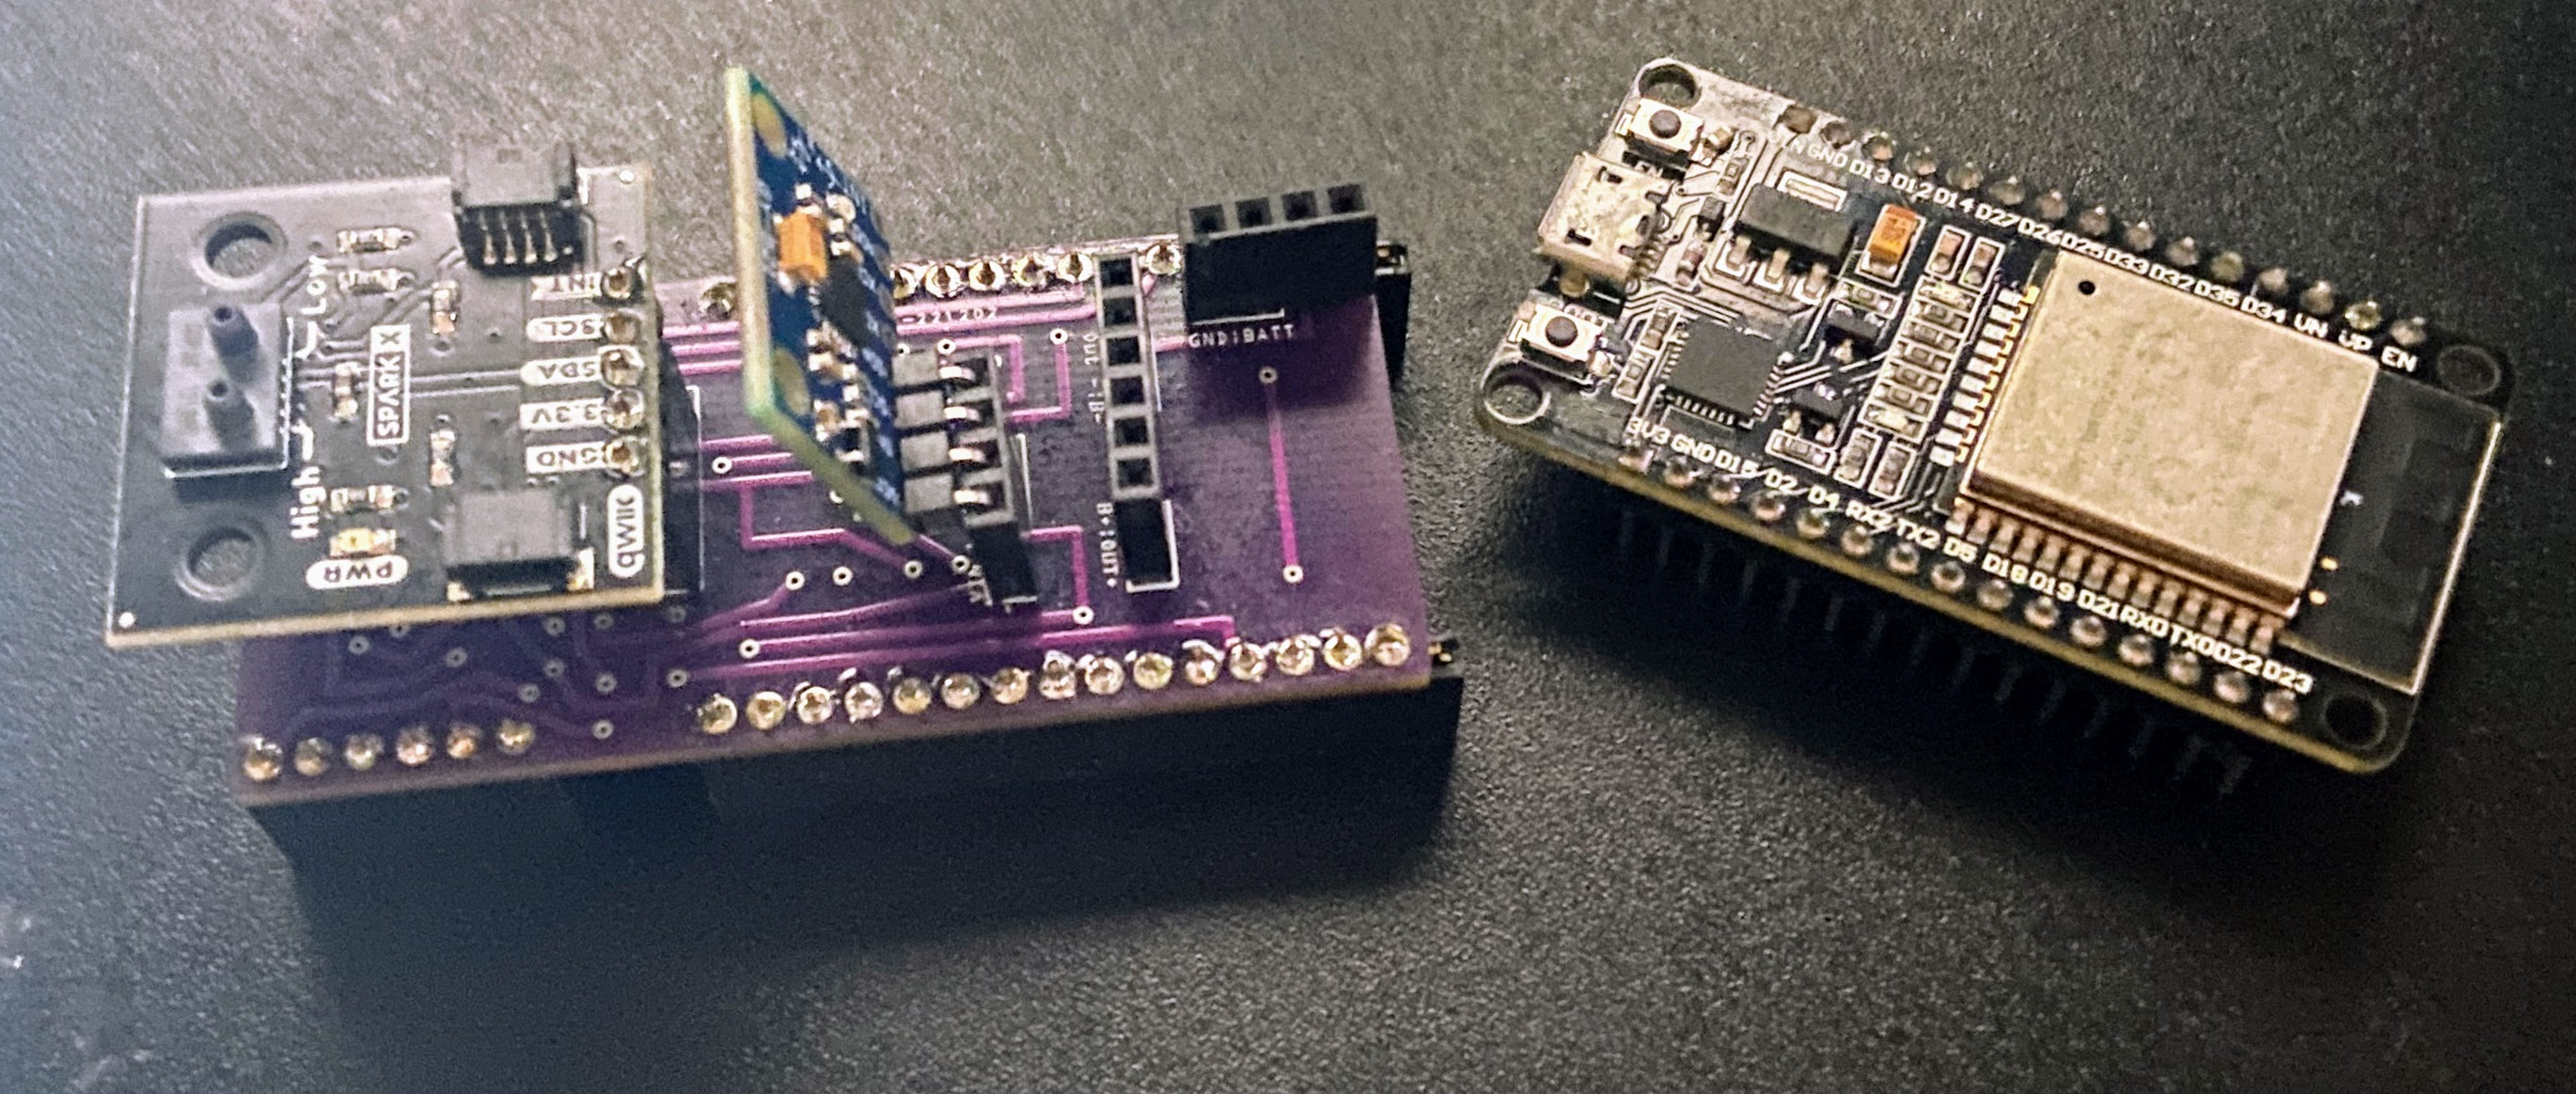
\includegraphics[scale=0.15]{diagrams/builtUnits/protoBoard.JPG}
    \caption{Prototype Socket Board for Version 1.3}
    \label{fig:protoBoard2}
\end{figure}


\subsection{I2C Snesors}

define and describe i2c and the sensors

\subsubsection{Gyroscope \& Accelerometer}

\begin{center}
    \begin{figure}
        \centering
        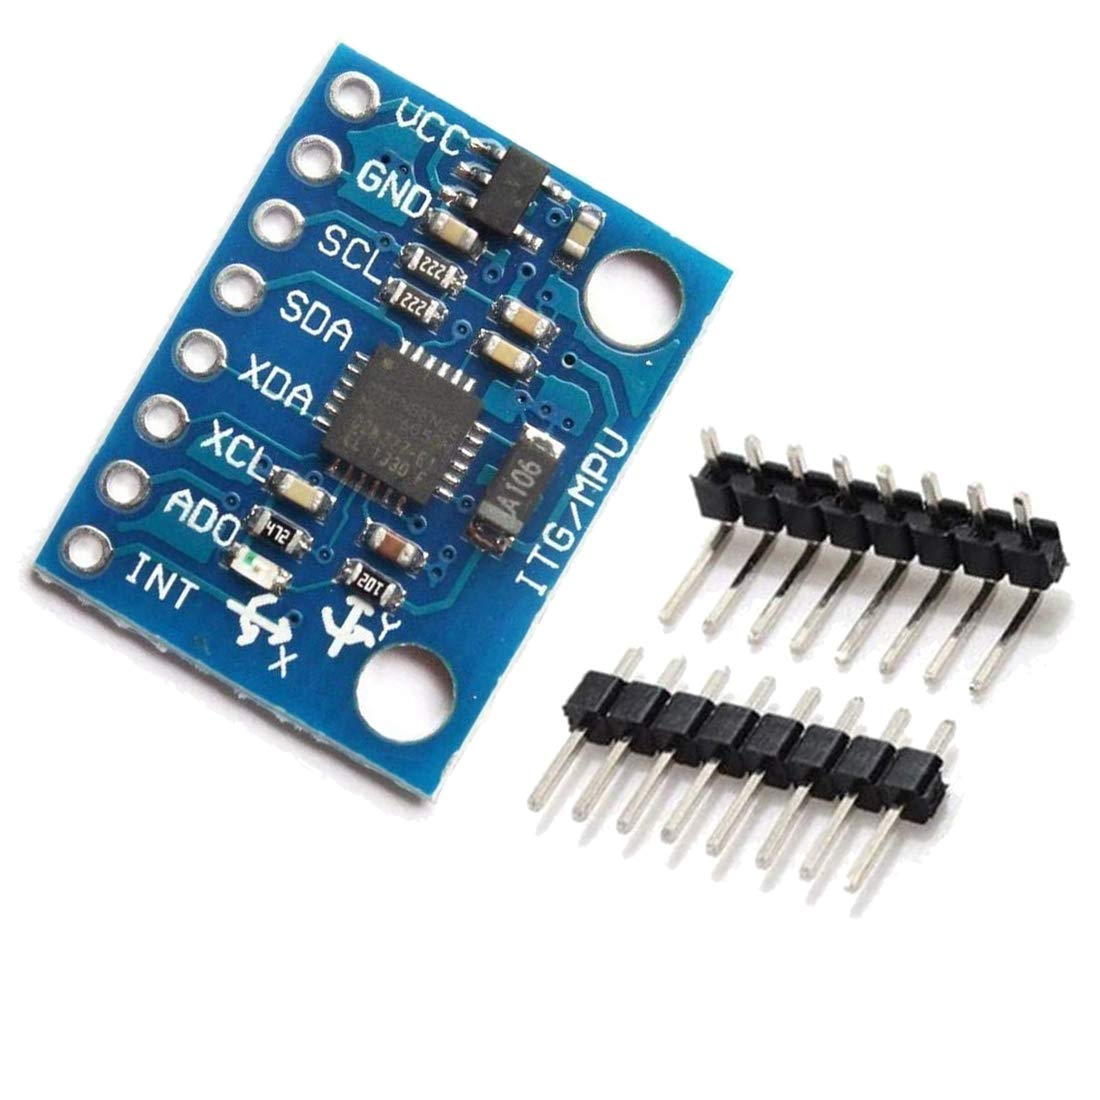
\includegraphics[scale=0.2]{diagrams/oem/6050.jpg}
        \caption{MPU-6050 Gyroscope and Accelerometer}
        \label{fig:6050}
    \end{figure}
\end{center}


\subsubsection{Differential Airflow Pressure \& Thermometer}

SDP-31
Originally released in 2017, this is the newest hardware component in the Bill of Materials. This unit detects differential airflow pressure between two points as well as temperature. Due to the SDP-3X line’s small form factor, the Sparkfun Qwiic connector break out board was selected for simple installation. Two small tubes are attached to the ports and used to measure the air pressure difference between the inside of the clarinet mouthpiece and the outside of the instrument.

\begin{center}
    \begin{figure}
        \centering
        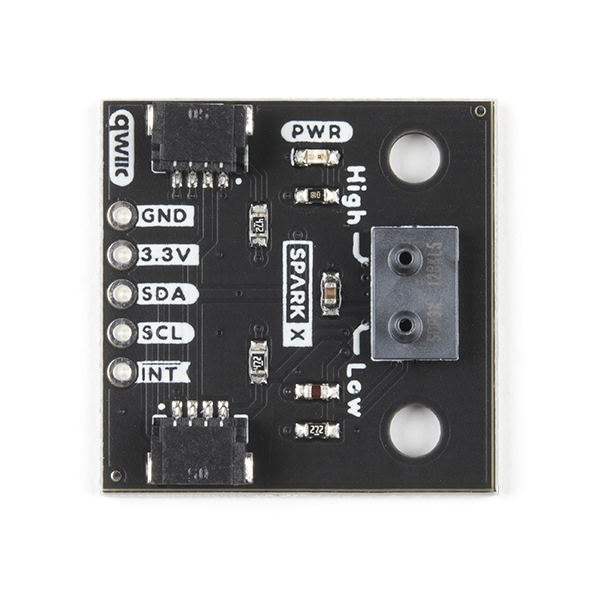
\includegraphics[scale=1.5, angle=90]{diagrams/oem/spd31.jpg}
        \caption{Sparkfun SDP-31 Differential Airflow Pressure Qwiic Connect Breakout Board}
        \label{fig:sdp-31}
    \end{figure}
\end{center}

Because of it’s higher accuracy, the SDP-31’s temperature sensor is utilized over the MPU-6050. Temperature is measured in degrees Celsius.



\section{Micro-Controller \& Power Distribution}

\subsection{ESP-32}
The Cyberinet contains a variety of useful sensors, however without the micro-controller, they become effectively useless in this context. In order to effectively manage all of the sensors and transmit the data, the Espressif ESP-32 DEVKIT V1 was ultimately selected for use with the Cyberinet. This board was selected for a handful of reasons, including:

\begin{itemize}
    \item Board's narrow size
    \item Large number of ports
    \item Arduino compatibility
    \item Wireless communications
\end{itemize}

The first two items on the list are closely related. While being narrower that comparable Arduino units, the ESP-32 DEVKIT V1 has 30 unique I/O Pins\footnote{Other versions of the DEVKIT have 36 GPIO pins. These boards are incompatible with the PCBs used in the Cyberinet.}. While four pins are dedicated to power distribution and another for the 'enable' functionality (EN), the remaining 20 can be utilized for sensors in a variety of ways. All of this potential functionality is compressed to just under 3 centimeters wide. Because of the ultimate physical design of the Cyberinet unit, having a large amount of accessible pins in a smaller unit was considered ideal. The DEVKIT V1 was preferred over the significantly smaller base chip to increase the simplicity of prototyping, repair, and future changes due to its OEM compatibility, and the popularity of the board among the community. The specific ship dimensions can be seen in figure \ref{fig:esp-32}

\begin{center}
    \begin{figure}
        \centering
        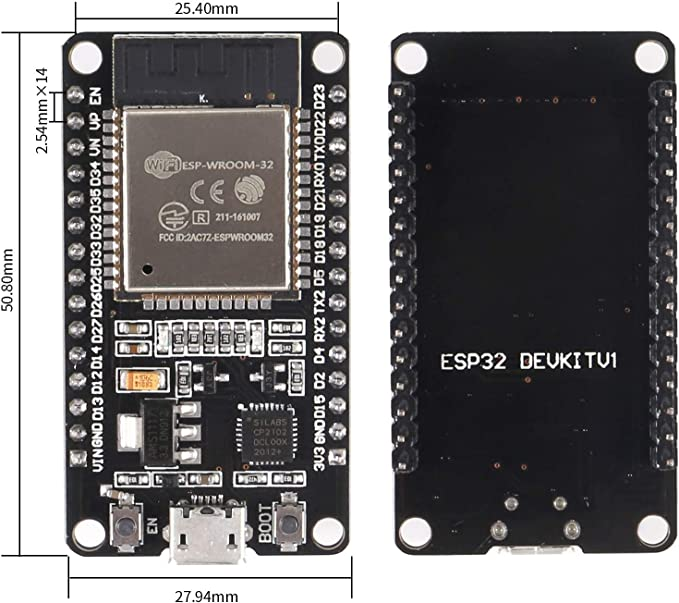
\includegraphics[scale=0.5]{diagrams/oem/esp-32.jpg}
        \caption{ESP-32 DEVKIT V1 micro-controller used in the Cyberinet}
        \label{fig:esp-32}
    \end{figure}
\end{center}

 

Because of the large number of Pulse-Width-Modulation-Controlled GPIO pins, the Cyberinet has the potential for a large number of sensors and expansions, but to help contain the form factor, only a handful are being utilized at any time. We can see the included sensors attached to the pins as shown below. More details about each of the sensors are discussed in each of the following sub-chapters. The labels in the figure below utilizes the pin labels that are printed on the DEKVIT V1. The placement of the shown pins are also shown in figure \ref{fig:esp-32}.

\begin{itemize}
    \item VIN: Power from Battery
    \item GND: Ground
    \item 2: Power LED
    \item 4: Togglable LED
    \item 12: Button 1
    \item 14: Button 2
    \item 21: Gyroscope and Airflow Data
    \item 22: Gyroscope and Airflow Clock
\end{itemize}

Both the Gyroscope and Airflow pressure sensors utilize the same pins. These are the I2C pins on the DEVKIT. More details will be discussed in the chapter discussing the Arduino programming, but it should be noted now that these sensors are able to utilize the same pins because they utilize different I2C addresses. The code is able to access these different addresses in sequence when collecting data.

The code written for the ESP-32 DEVKIT was created using the Arduino IDE and coding language. For similar reasons to the choice of the DEVKIT, this was done for greater accessibility and simplicity in programming. More details about the Arduino Code are discussed later, and the code as a whole is included in the appendices.

The final item from the initial list was the wireless capabilities. The ESP-32 is able to perform serial communications with a connected computer via a micro-USB or USB-C cable (depending on the board version). While useful, the goal of the Cyberinet is to provide affordable instrument augmentation with minimal alterations to the clarinetist's performance practice. Towards this goal, minimizing the number of extra cables was a design concern from the first prototypes. By utilizing the built-in Bluetooth capabilities, the performer is able communicate with the computer easily while meeting this requirement.

The ESP-32 also has WiFi connectivity capabilities which may be involved in a future version, but at the current time is currently not utilized. The DEVKIT is able to support Bluetooth version 4.2 and Low Energy protocols for local wireless communication. This allows for the Cyberinet to easily pair with any computer that it has previously connected to using the BTSerial Arduino library. A code library that brings the normal wired Serial functionality to the Bluetooth functionality.

While not as powerful as the most up-to-date Bluetooth hardware, the DEVKIT's version 4.2 allows the Cyberinet to connect to a computer from up to 200 feet away with a max data transfer speed of 1 Mbps. While these values do fluctuate depending on the performance venue layout, and have a minor impedance from the case of the Cyberinet itself, the performance statistics are still high enough for a large majority or performance areas. This will be discussed more in the chapter discussion the music compositions and performance with the Cyberinet. 


\subsection{Power Distribution}
In order to power the entire system, a lithium ion polymer battery is included inside the hardware. In order to charge the unit, users can utilize the provided USB-C cable and power adapter to the port located on the bottom of the unit. % show pic of charging port


All power distribution for the Cyberinet is handled with a TP-4056 Type C chip, shown in figure \ref{fig:tp5046}. The version containing a USB-C connector was chosen over the Micro-USB connector for two main reasons. The first being a desire for consistent, modern connectors in the device, and the second reason being that this upgraded version allows for both battery charging and distribution. The older Micro-USB chips only allow for battery charging.


\begin{center}
    \begin{figure}
        \centering
        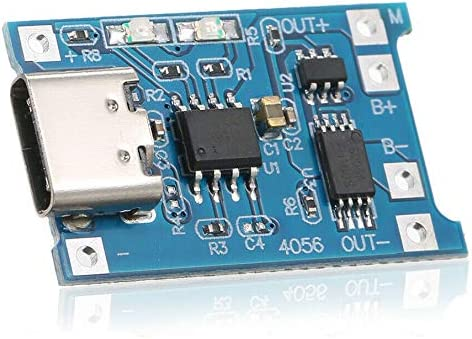
\includegraphics[scale=0.5]{diagrams/oem/4056.jpg}
        \caption{The TP-4056 Power Distribution Chip used in the Cyberinet}
        \label{fig:tp5046}
    \end{figure}
\end{center}

By connecting the battery to the connections labeled B+ and B-, and connecting the Vin and GND pins of the ESP-32 to the OUT+ and OUT- on this board, the Cyberinet is able to receive all required power through the single chip. The power button is soldered into the connection between the battery and the TP-4056, and will automatically power the Cyberinet when activated\footnote{Because of the placement of the power switch, the device will have to be powered on while charging. This can be easily verified by the onboard LED's}. 

When the battery is depleted, it must be connected to a power source via this USB-C port to be able to fuly charge. From an empty charge, the unit can take between one and three hours to fully charge. The exact times can vary depending on the power adapter and whether any additional accessories are connected. 

The battery included is rated for 1200 mAh as an improvement over the 320 mAh battery used for initial testing and prototyping. This size battery allows the Cyberinet to have as much run time as possible while still maintaining the size characteristics of the hardware electronics. The approximate run times are as follows:

\begin{itemize}
    \item Powered on, not connected: 5 hours.
    \item Powered on, Bluetooth connected, no expansions added: 5-6 hours.
    \item Powered on, Bluetooth connected, expansions added: 4-5 hours.
\end{itemize}


It should be noted that the device can also run when connected directly to the wall socket power supply. This will also charge the battery, which, while resulting in yet another wire, can result in an indefinite run time.

% below doesnt actually happen. uncomment when .ino code allows for it to happen
% When the battery capacity becomes critically low, the device will stop transmitting data, however the LEDs may stay on due to residual amounts of electricity present in the system. To avoid accidental drop outs during a performance, it is recommended to fully charge the device prior to any performances to avoid this. When the battery reaches 20\% charge, the red LED on the device will illuminate, and then flash as shown below:

% \begin{itemize}
%     \item 15\%: 1 flash
%     \item 10\%: 2 flashes
%     \item 5\%: 3 flashes
% \end{itemize}

\subsection{Optional Expansion Sensors}
In addition to the built-in sensors, the Cyberinet utilizes a variety of optional expansions that can be implemented as needed to customize the array of sensors. The main expansion unit contains two momentary push buttons and is discussed in greater detail below.

\subsubsection{Button Expansion}

\begin{center}
    \begin{figure}
        \centering
        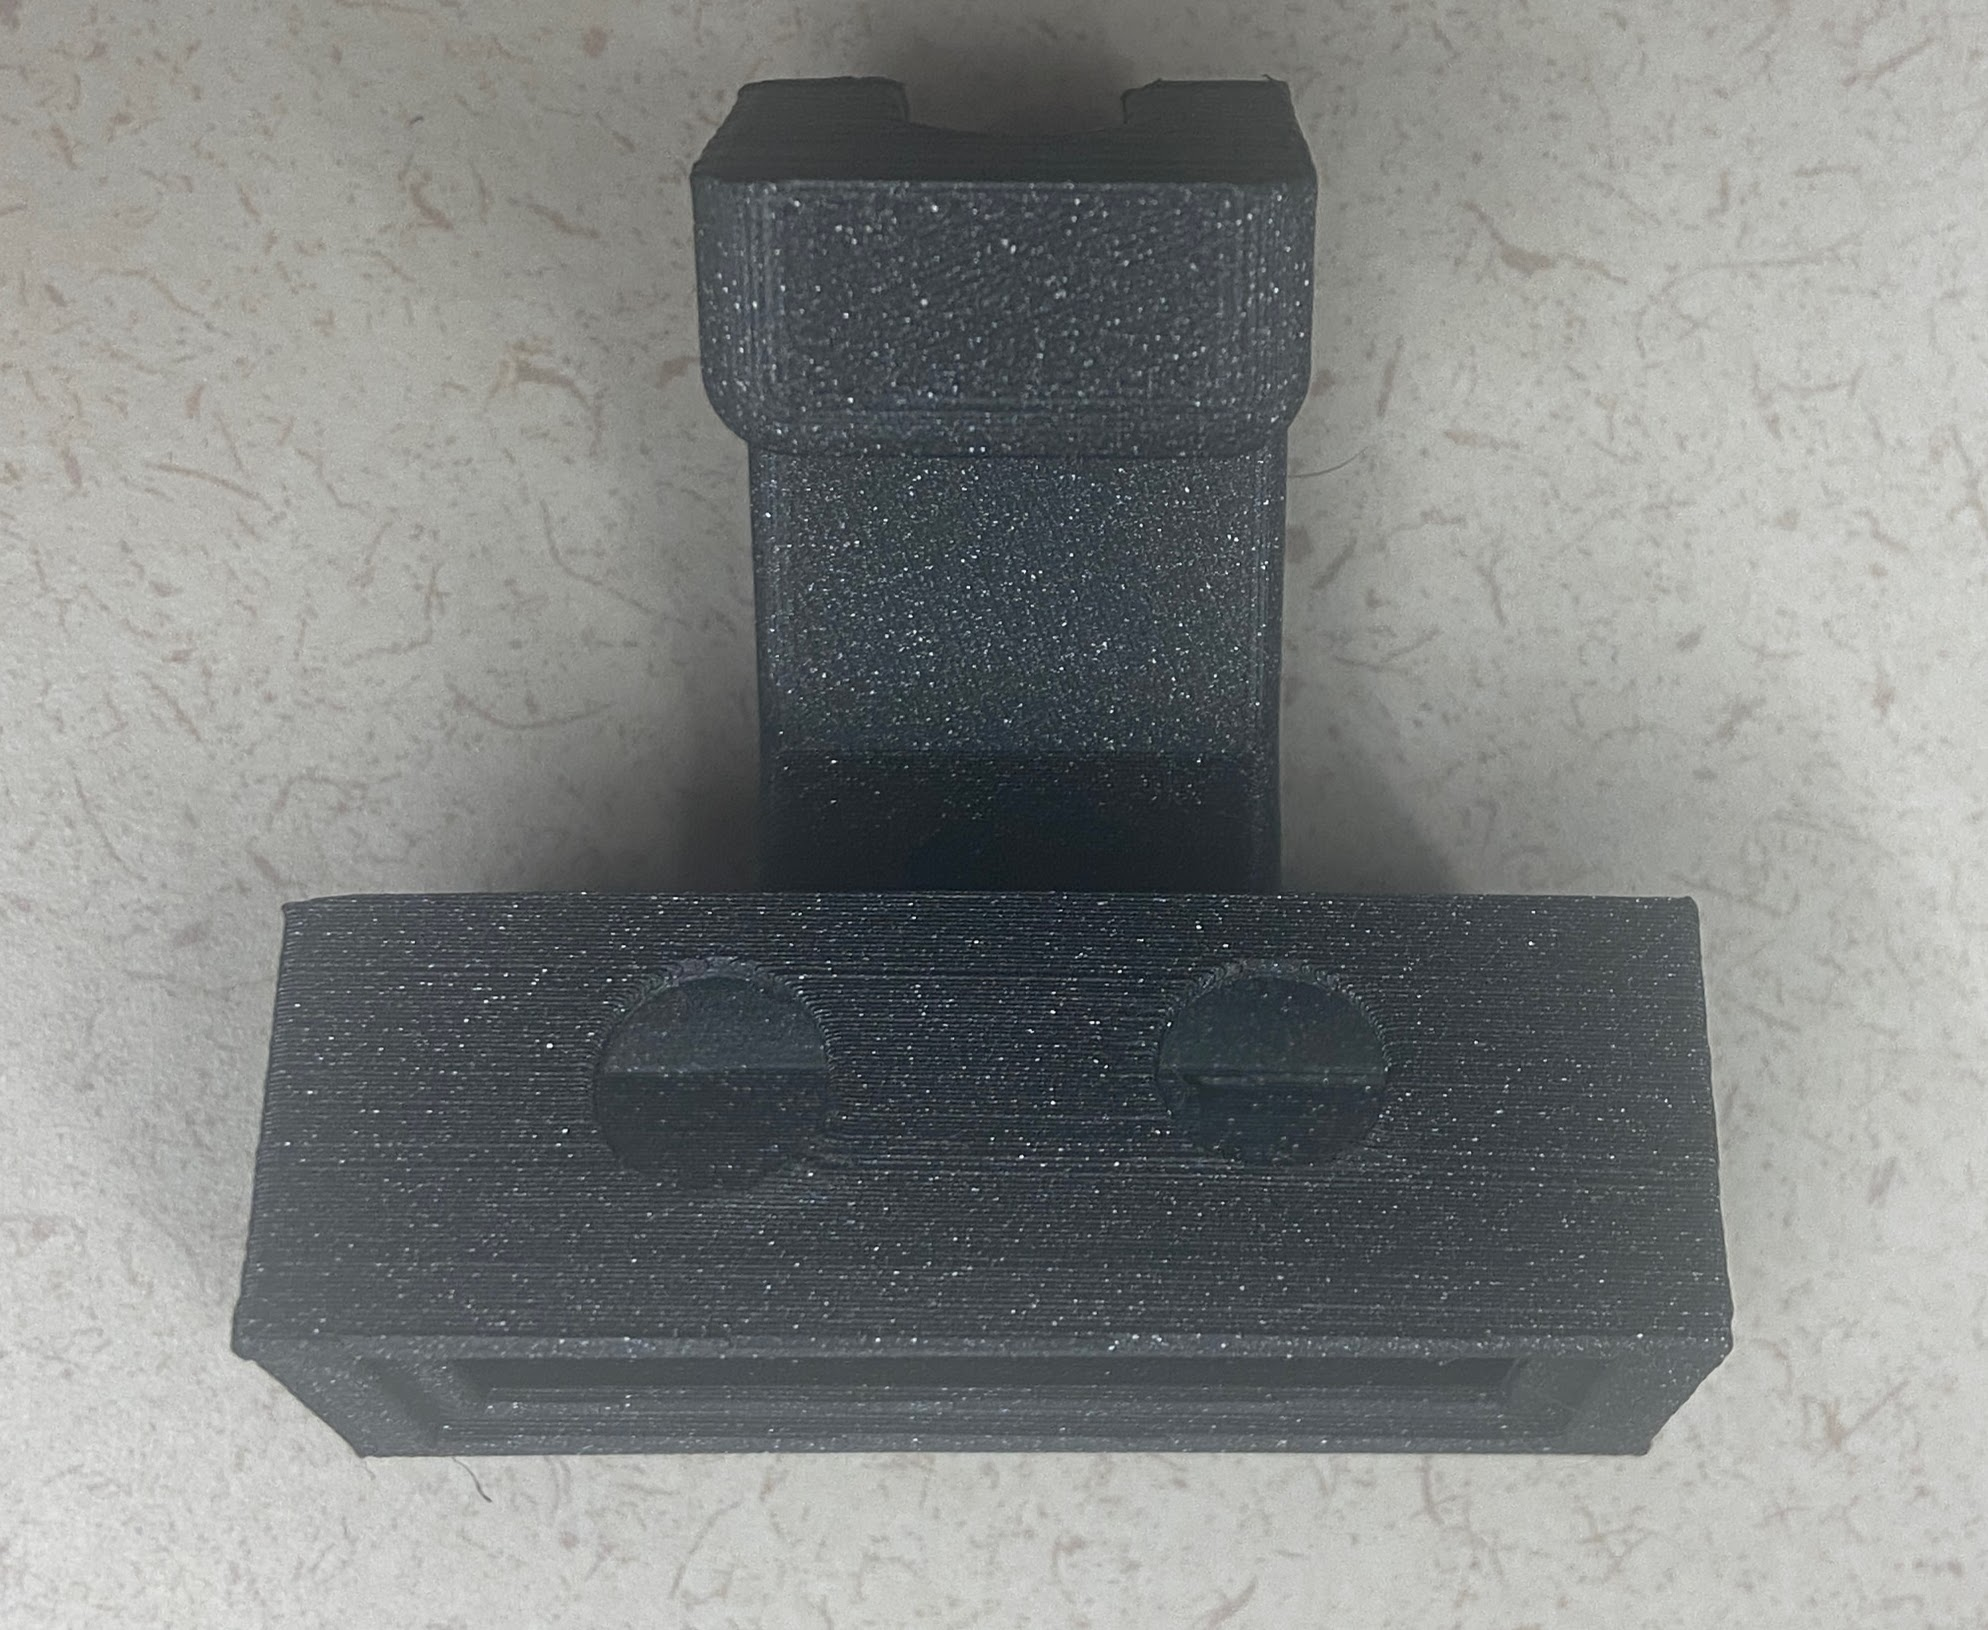
\includegraphics[scale=0.1]{diagrams/builtUnits/buttonhousingEmpty.JPG}
        \caption{Empty 3D-printed thumb rest with housing for buttons below.}
        \label{fig:buttonThumbrest}
    \end{figure}
\end{center}

These attachments are optional and not needed for the Cyberinet main unit to be functional and are intended to only be connected when needed for a particular performance. All the expansions connect utilizing a standard USB-C connector. However, these units do not utilize the USB protocol, so both the main unit and expansions cannot be connected to a computer via these ports. Because the Cyberinet does not communicate to these using USB protocol, not all USB-C cables can be used for this, however the vast majority can. While a set of USB-C cables that are functional is included with the full Cyberinet set of hardware, The main reason for utilizing this connector is for the end-user to be able to supply their own cables of various lengths depending on their needs. 


\begin{center}
    \begin{figure}
        \centering
        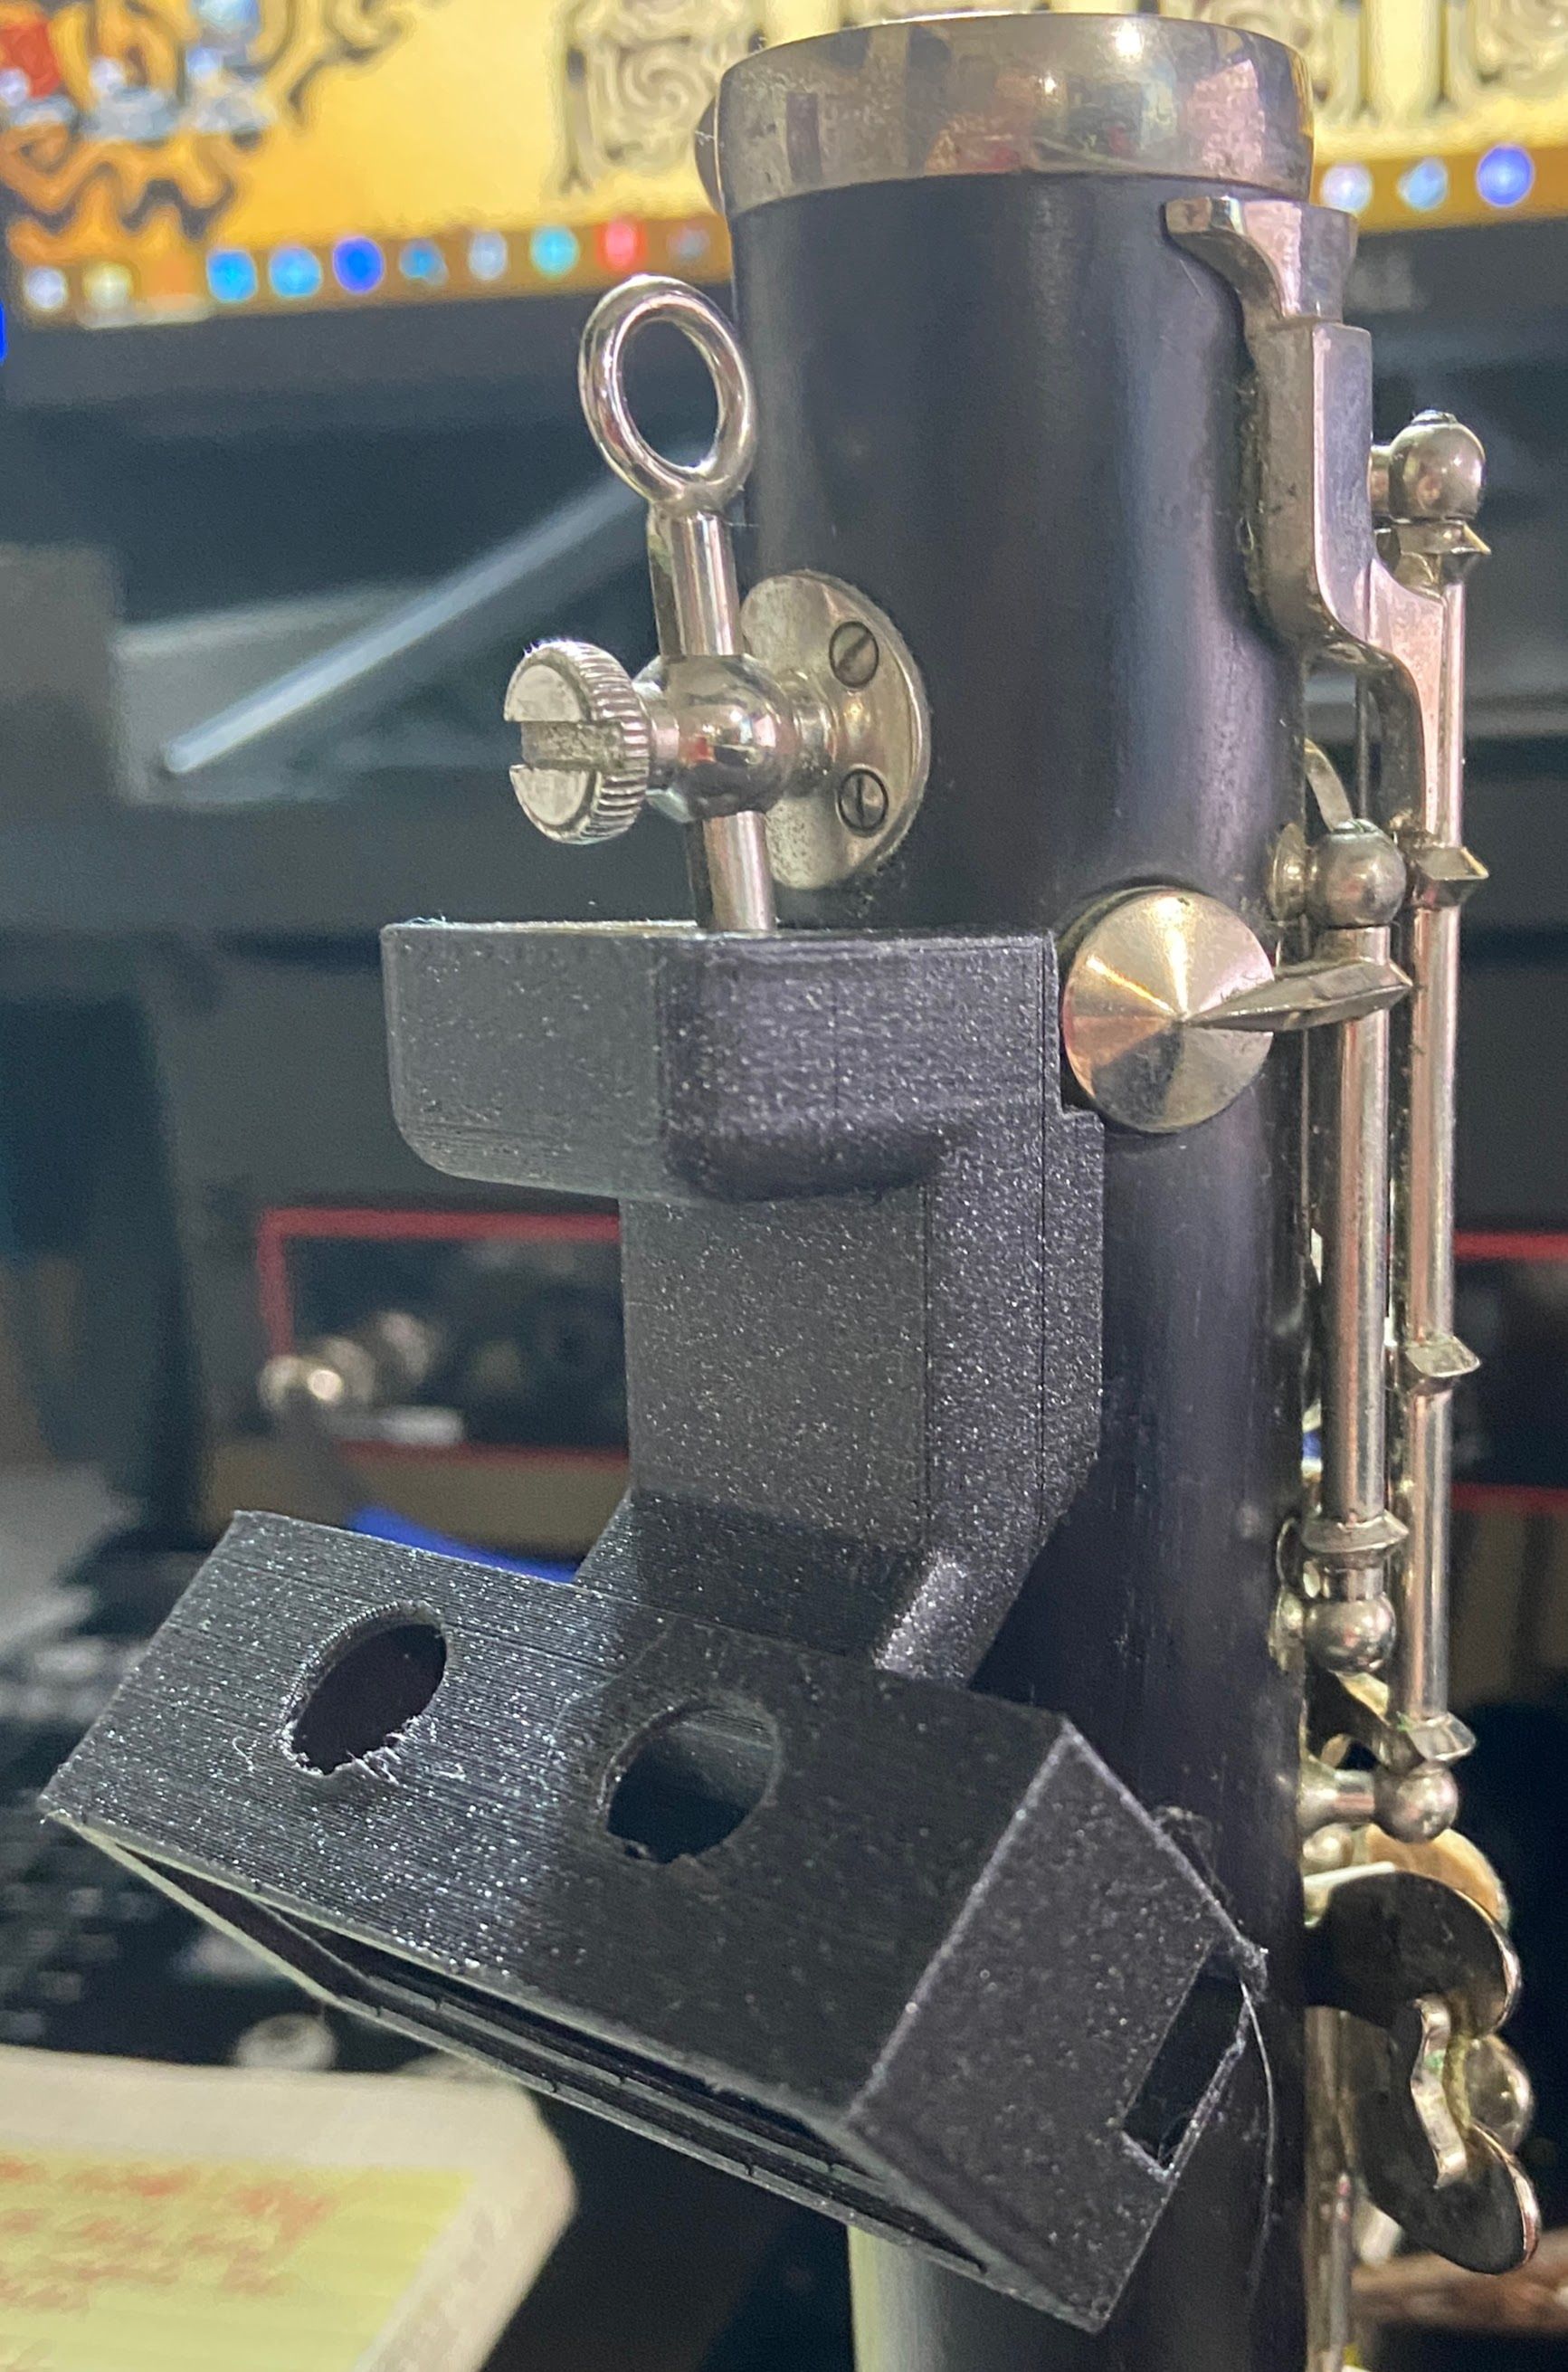
\includegraphics[scale=0.08]{diagrams/builtUnits/thumbOnInst.JPG}
        \caption{Empty Button Expansion placed on a Clarinet thumb rest}
        \label{fig:thumbOnCase}
    \end{figure}
\end{center}

This board, while optional, is incredibly useful for a performer on stage. They can access the buttons using their right thumb when performing. This maneuver is easier when utilizing a neck strap, so the performer can place the buttons elsewhere if they like using a longer connector cable. The closeness between the buttons and thumb rest is shown in figures \ref{fig:buttonThumbrest} and \ref{fig:thumbOnCase}\footnote{The case has been revised since the initial picture was taken. The small rectangular hole for the connection cable has been moved to the left side to avoid potential collisions with the performer's hand.}. Each button also contains a single, colored LED built into it to provide feedback to the performer. By default, the lights are only illuminated when the button is pressed. The Cyberinet simply detects whether a button has been pressed and transmits that data as a Boolean value to the computer. Using a program such as Max, the user can have the buttons achieve functions from near limitless hypothetical list of options. For this project, the buttons were used to trigger microphone recording and buffer playback, however objects that take the button input and move between various presets, trigger DSP, and turn pages of a score have also been developed and included in the software bundle for this project.

\subsubsection{Other Expansions}
At the time of writing, only the button expansion has been developed and tested completely. However, in-progress plans for a continuing range of expansions exist. These include the sensors described here.

The joystick expansion is relatively simple. It is designed to receive data from the single button and two potentiometers of a standard joystick. The PCB diagram shown in figure \ref{fig:jsPCB} shows the simplicity of this setup.Power and ground are received and fed to both the joystick as well as the power indicator LED. The values from the horizontal position, vertical position, and button are all returned to the ESP-32 on pins 33, 32, and 35 respectively. When transmitting to the computer, the data receives the labels exp1, exp2, and exp3.\footnote{All expansion units receive the same label with a different number because they are hot-swapable. This removes the need for a the unit to have to identify the expansion and apply the appropriate label.}

\begin{figure}
    \centering
    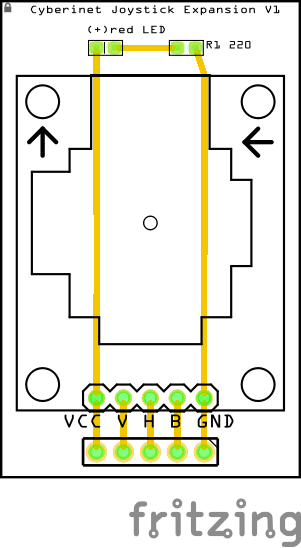
\includegraphics{diagrams/PCBs/thumbPCBv1.png}
    \caption{Joystick Expansion PCB diagram}
    \label{fig:jsPCB}
\end{figure}

As shown in the middle of the board, there is space for a daughter board to be attached. This is the Sparkfun BOB-09110 breakout board, which serves as the interface between the COM-16273 Joystick Deluxe the board shown in figure \ref{fig:jsPCB}. When all soldered, the voltages are passed through to the 5 pins at the bottom, which are wired with a ribbon cable to the USB-C port similar to the button expansion. The deluxe joystick was selected because of its higher-quality construction compared to other joysticks on the market, and the ability to easily swap tops to allow for a variety of interface options and feelings for the performer.

\begin{figure}
    \centering
    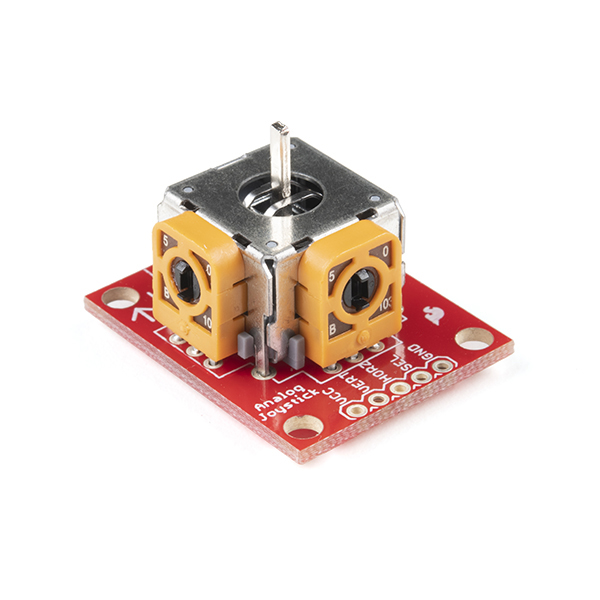
\includegraphics{diagrams/oem/16273-Thumb_Joystick_-_Deluxe-03.jpg}
    \caption{Joystick on BOB-09110 Breakout Board}
    \label{fig:js2}
\end{figure}

The element of the unit remaining to be designed at this moment is the 3D printed housing. This is intended to attach to the clarinet in place of the button expansion, allowing for thumb control on the thumb rest.


The Volume Detection unit contains uxcell Microphone Sound Sensor Voice Detection Module. Like the Button Expansion, this unit is housed in a 3D printed case and connects to the Main unit with a USB-C cable. The PCB diagram shown in figure \ref{fig:micExPCB} is perhaps the least complex of all of the boards created so far. It essentially acts as an interface for the breakout module and the USB-C connector. Like the joystick and main PCBs, there is a place to include the power indication LED. The module will sit on the majority of empty space on the board, and should be pointed towards the desired pickup area. If loose, a little glue is used to help hold the module down to the PCB here. 

\begin{figure}
    \centering
    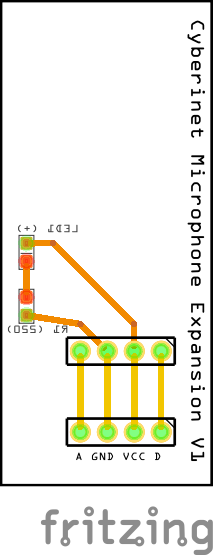
\includegraphics[angle=90]{diagrams/PCBs/micBasic_pcb.png}
    \caption{Microphone Expansion base PCB}
    \label{fig:micExPCB}
\end{figure}

This unit is designed to respond to the volume of the local area, and is designed to be placed in a variety of different areas. By placing the sensor at different distances from the performer or speakers, the sensor can more or less sensitively respond to the volume. The sensitivity can be adjusted with an on-board potentiometer and screwdriver. The user is only limited by the length of USB-C cable they can utilize. The Cyberinet detects when the volume at the sensor exceeds the given threshold from the on-board potentiometer, and transmits the data as a Boolean value to the computer in a similar manner to the Button Expansion. Future revisions will explore the uxcell Microphone Sound Sensor Voice Detection Module's analog outputs, but for now version 1 will only be utilizing the digital output. Ground and power connect to the middle two pins, and the data is returned on the pin marked D in figure \ref{fig:micExPCB}. This data is transmitted using the label exp1. 

Like the joystick, the 3D case is the final element keeping this unit from being further developed at the time of writing. The case is intended to entirely cover the microphone with the exception of holes for sound pickup, threshold adjustment, and viewing the LED. The unit is also intended to have a clip that can be used to attack it to various objects such as a music stand.

A few other planned expansion units are described at the end of this chapter.

\section{Physical Design}
In order to minimize the total number of parts required for the Cyberinet, the electronics are housed in a newly designed plastic unit. This Main Unit is intended to replace the barrel and mouthpiece of the original instrument when in use. In addition to the main unit, the Button Expansion as well as any future expansions have a 3D printed body in order to control the expansion's ergonomics and protect the electronics.

\begin{center}
    \begin{figure}
        \centering
        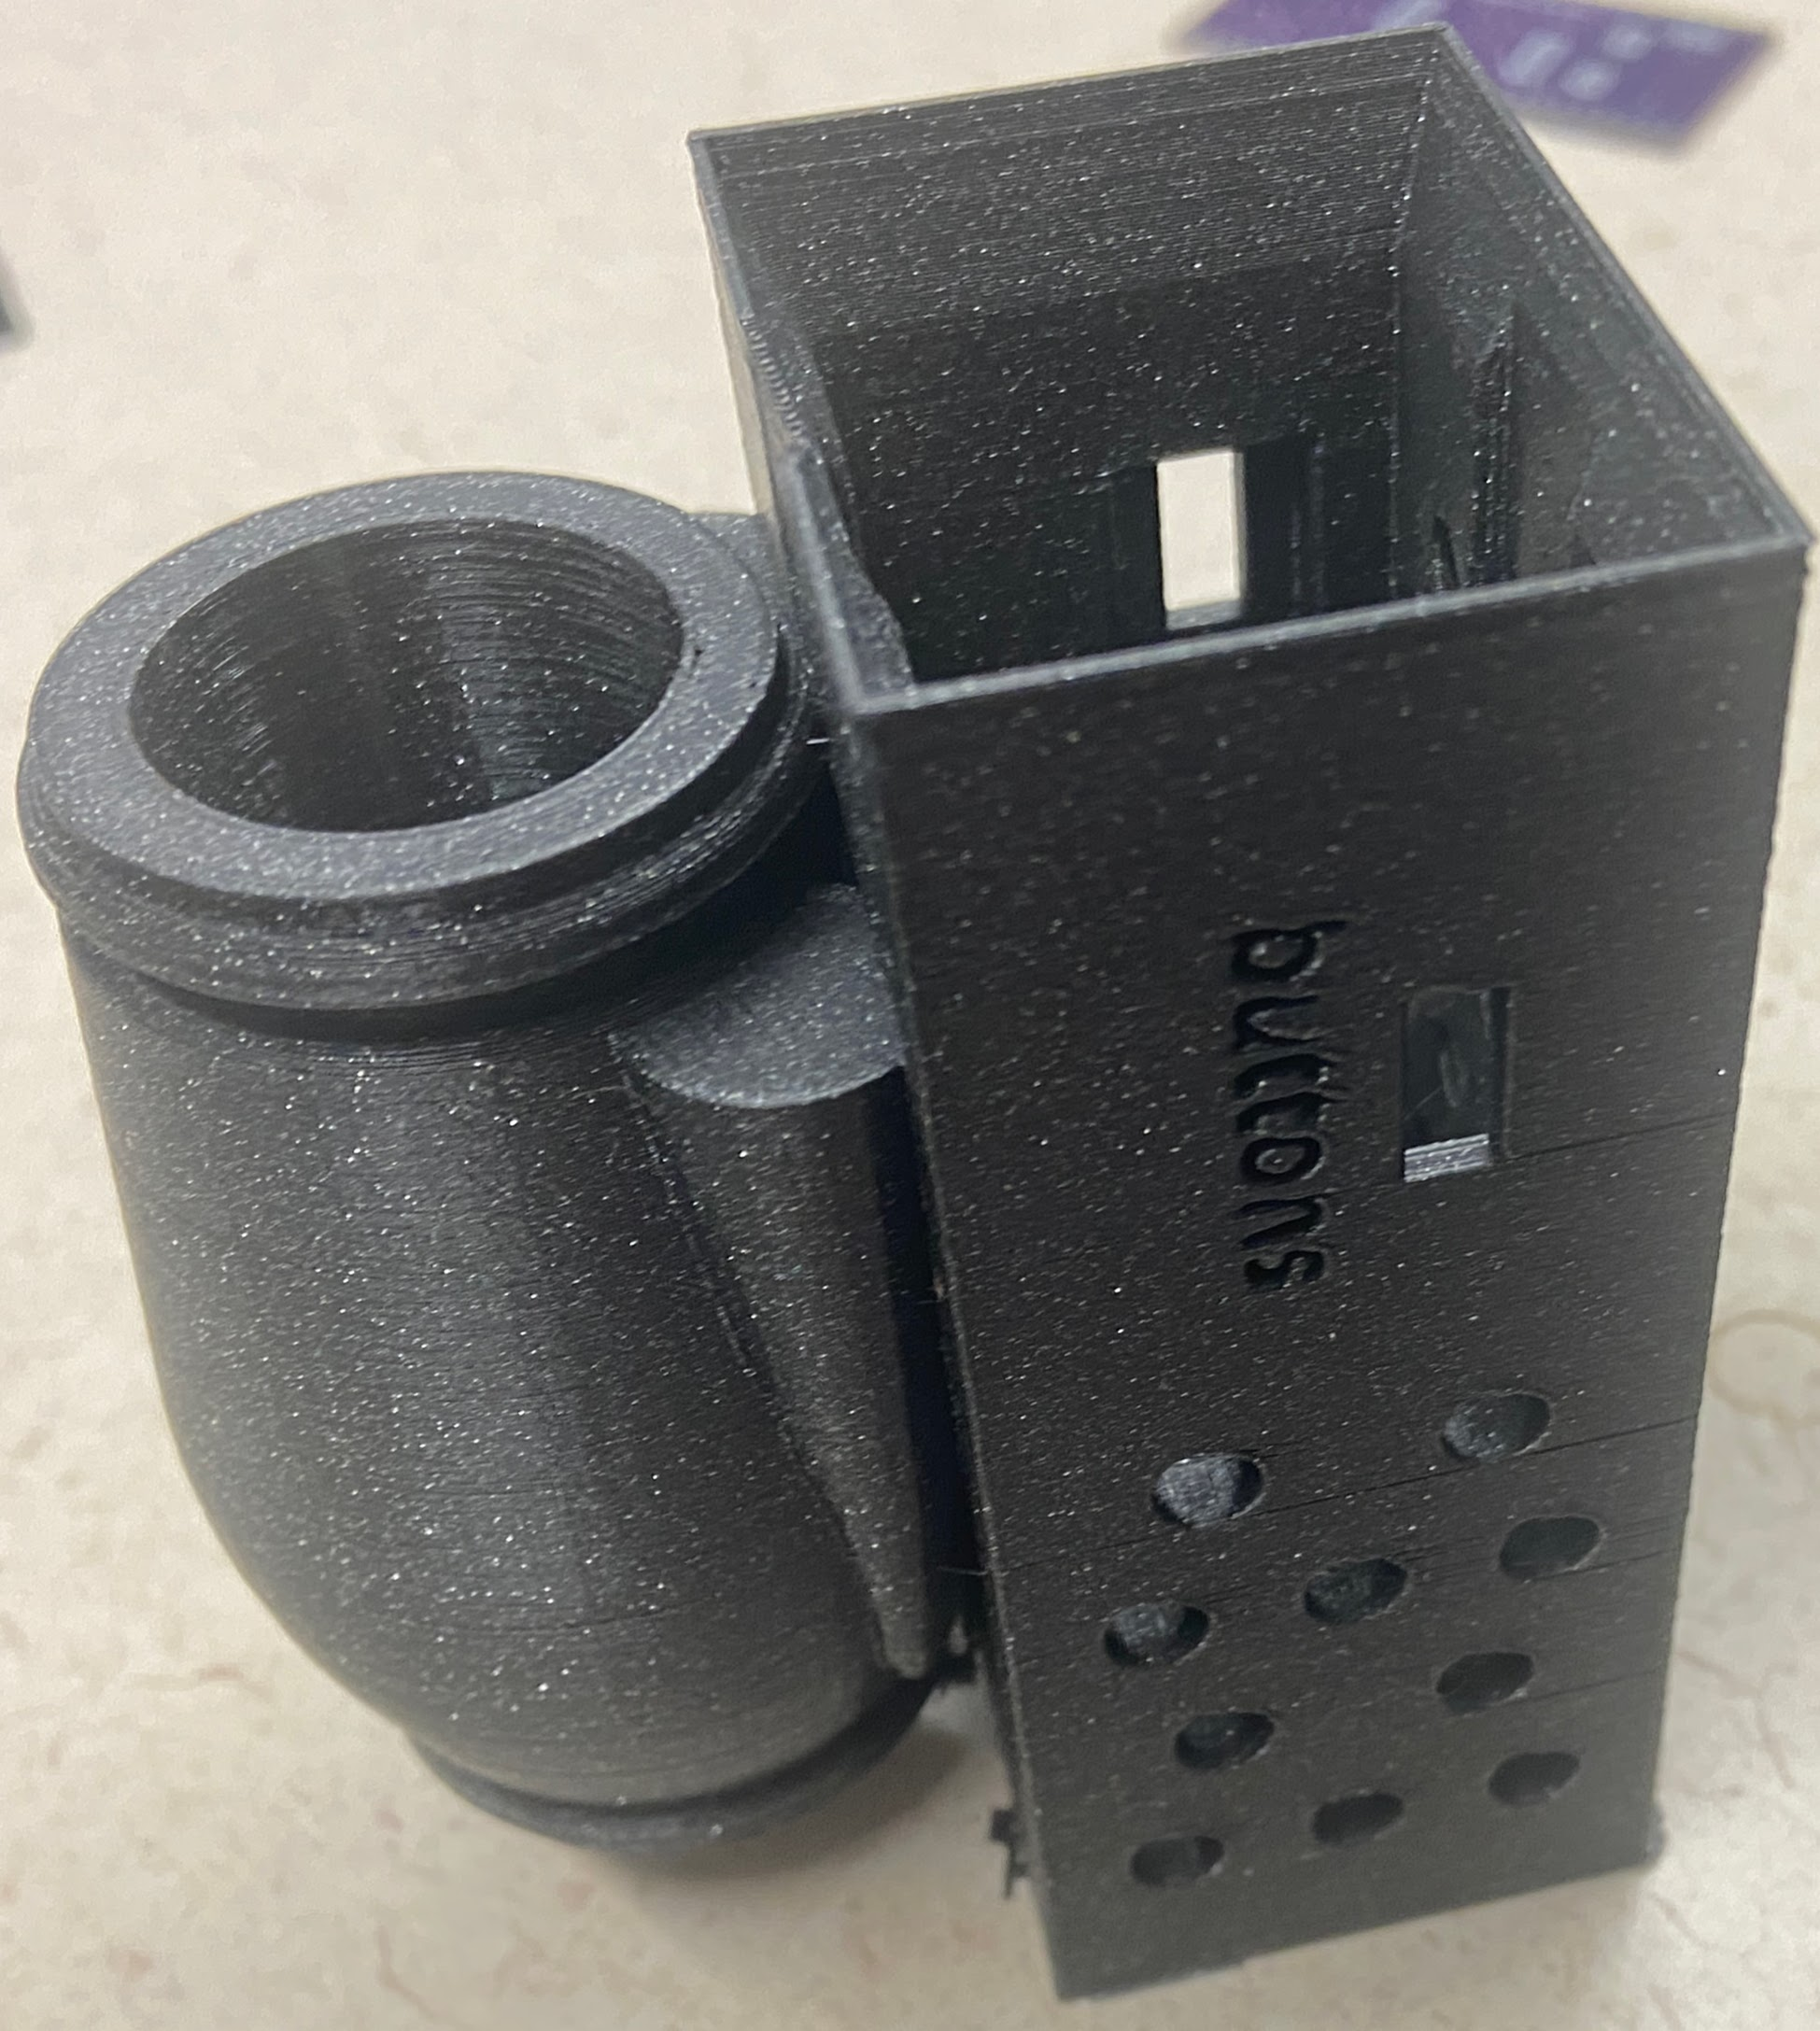
\includegraphics[scale=0.1]{diagrams/builtUnits/emptyCase.JPG}
        \caption{Empty 3D Printed Cyberinet Housing}
        \label{fig:cybernetCase}
    \end{figure}
\end{center}

All materials are printed using either PLA or PetG material during prototyping. These materials were chosen for their relative low cost, ease of production, and density. For the final version, PLA was utilized because the sound quality of the material most closely resembled that of the original clarinet. All parts were printed on an Original Prusa i3 MK3S+. Because of the testing of different materials, several images in this document may be in largely varying colors. The final version was printed to be black or dark grey, however future revisions could see an option for custom colors when printing. 

While it is intended to remove the Clarinet's uppermost parts and replace them with the Cyberinet when needed, it is possible to perform using the hardware while powered off for a traditionally acoustic performance. The usage of this feature is at the discretion of the performer.

\section{Main Unit Assembly}

The main unit of the Cyberinet is designed to replace the uppermost portions of a B-flat clarinet: The barrel and mouthpiece. As shown in figure \ref{fig:cybernetCase}, the electronic components are housed in the box on the side of the instrument. Placing the electronics here allows for the unit to be easily adjusted for tuning or be easily removed as needed. The box was made as small as possible, but it still contains all of the electronic components, excluding those in any external add-on components. 

The electronics were housed in the upper portion of the clarinet for two main reasons. The more minimal of the reasons is that the differential airflow pressure is much greater in the clarinet before the air can escape through the key holes. By locating the sensor here a wider range of values are possible than if it was located lower on the clarinet's tube. However, this could be remedied with additional tubing if the location of a unit needed to be otherwise located. Speculating on this is outside of the scope of this document however.

To assemble a Cyberinet main unit, first the case must be 3D printed. Because of the process of 3D printing and the necessary thickness of the material needed to preserve sound quality, the printing process takes approximately 12 hours to complete. Because of this, it is recommended to begin printing the units first, then work while the case is being completed by the printer.

All components are connected utilizing a custom printed circuit board. This is done to help connect all of the various pins for data collection and power distribution in as small of a space as possible. The PCB is shown in figure \ref{fig:mainUnitPCB}.

\begin{center}
    \begin{figure}
        \centering
        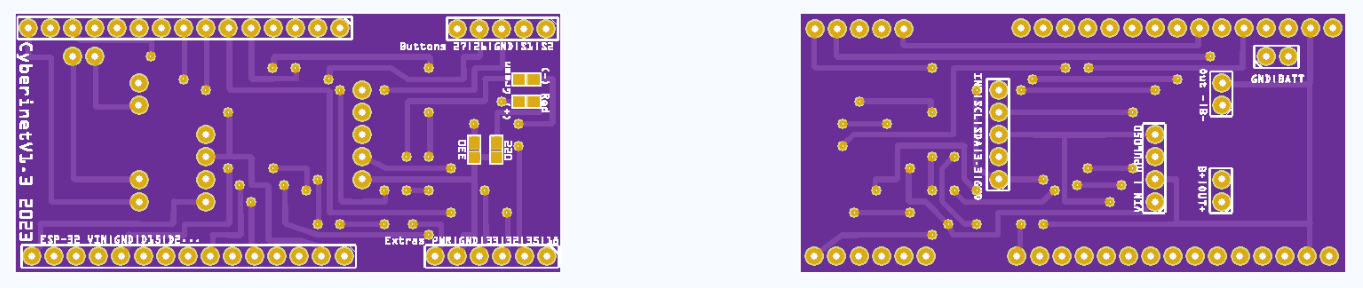
\includegraphics[scale=0.6]{diagrams/PCBs/cyberinetPCB.png}
        \caption{Cyberinet Version 1.3  Main Unit PCB Diagram}
        \label{fig:mainUnitPCB}
    \end{figure}
\end{center}

As shown in the following breakdown, assembling the Cyberinet must be done by working with the smallest components and working up to the larger ones. This is because several components are placed over other ones and it becomes exponentially harder to assemble a Cyberinet should one have to begin working around the placement of a sensor or remove a chip to adjust or repeat a step\footnote{It is recommended to pause and check the connections after soldering each component for this reason as well}.

First, the Surface-Mounted components are soldered onto the main board. These include the 2 on-board LEDs and their accompanying resistors. Following this, ribbon cables and the USB-C and JST connectors are then soldered into place on the PCB. The third step is to solder the power distribution (TP-4056), gyroscope (MPU-6050) and airflow pressure (SDP-31) chips into place. The white silkscreen rectangles show which side of the PCB each component belongs on, and the text indicates which orientation is needed for each component to help ensure a correct alignment.

The airflow pressure sensor (SPD-31) is lifted away from the PCB with the use of a pin header. This is done to avoid any accidental shorts between the contacts on the two boards. While not required, this can be done to the gyroscope (MPU-6050) as well. The final soldering step is to connect the ESP-32. Because of its size, this chip is kept opposite from the sensors and is also lifted using pin headers for the same reason as the SDP-31.

\begin{center}
    \begin{figure}
        \centering
        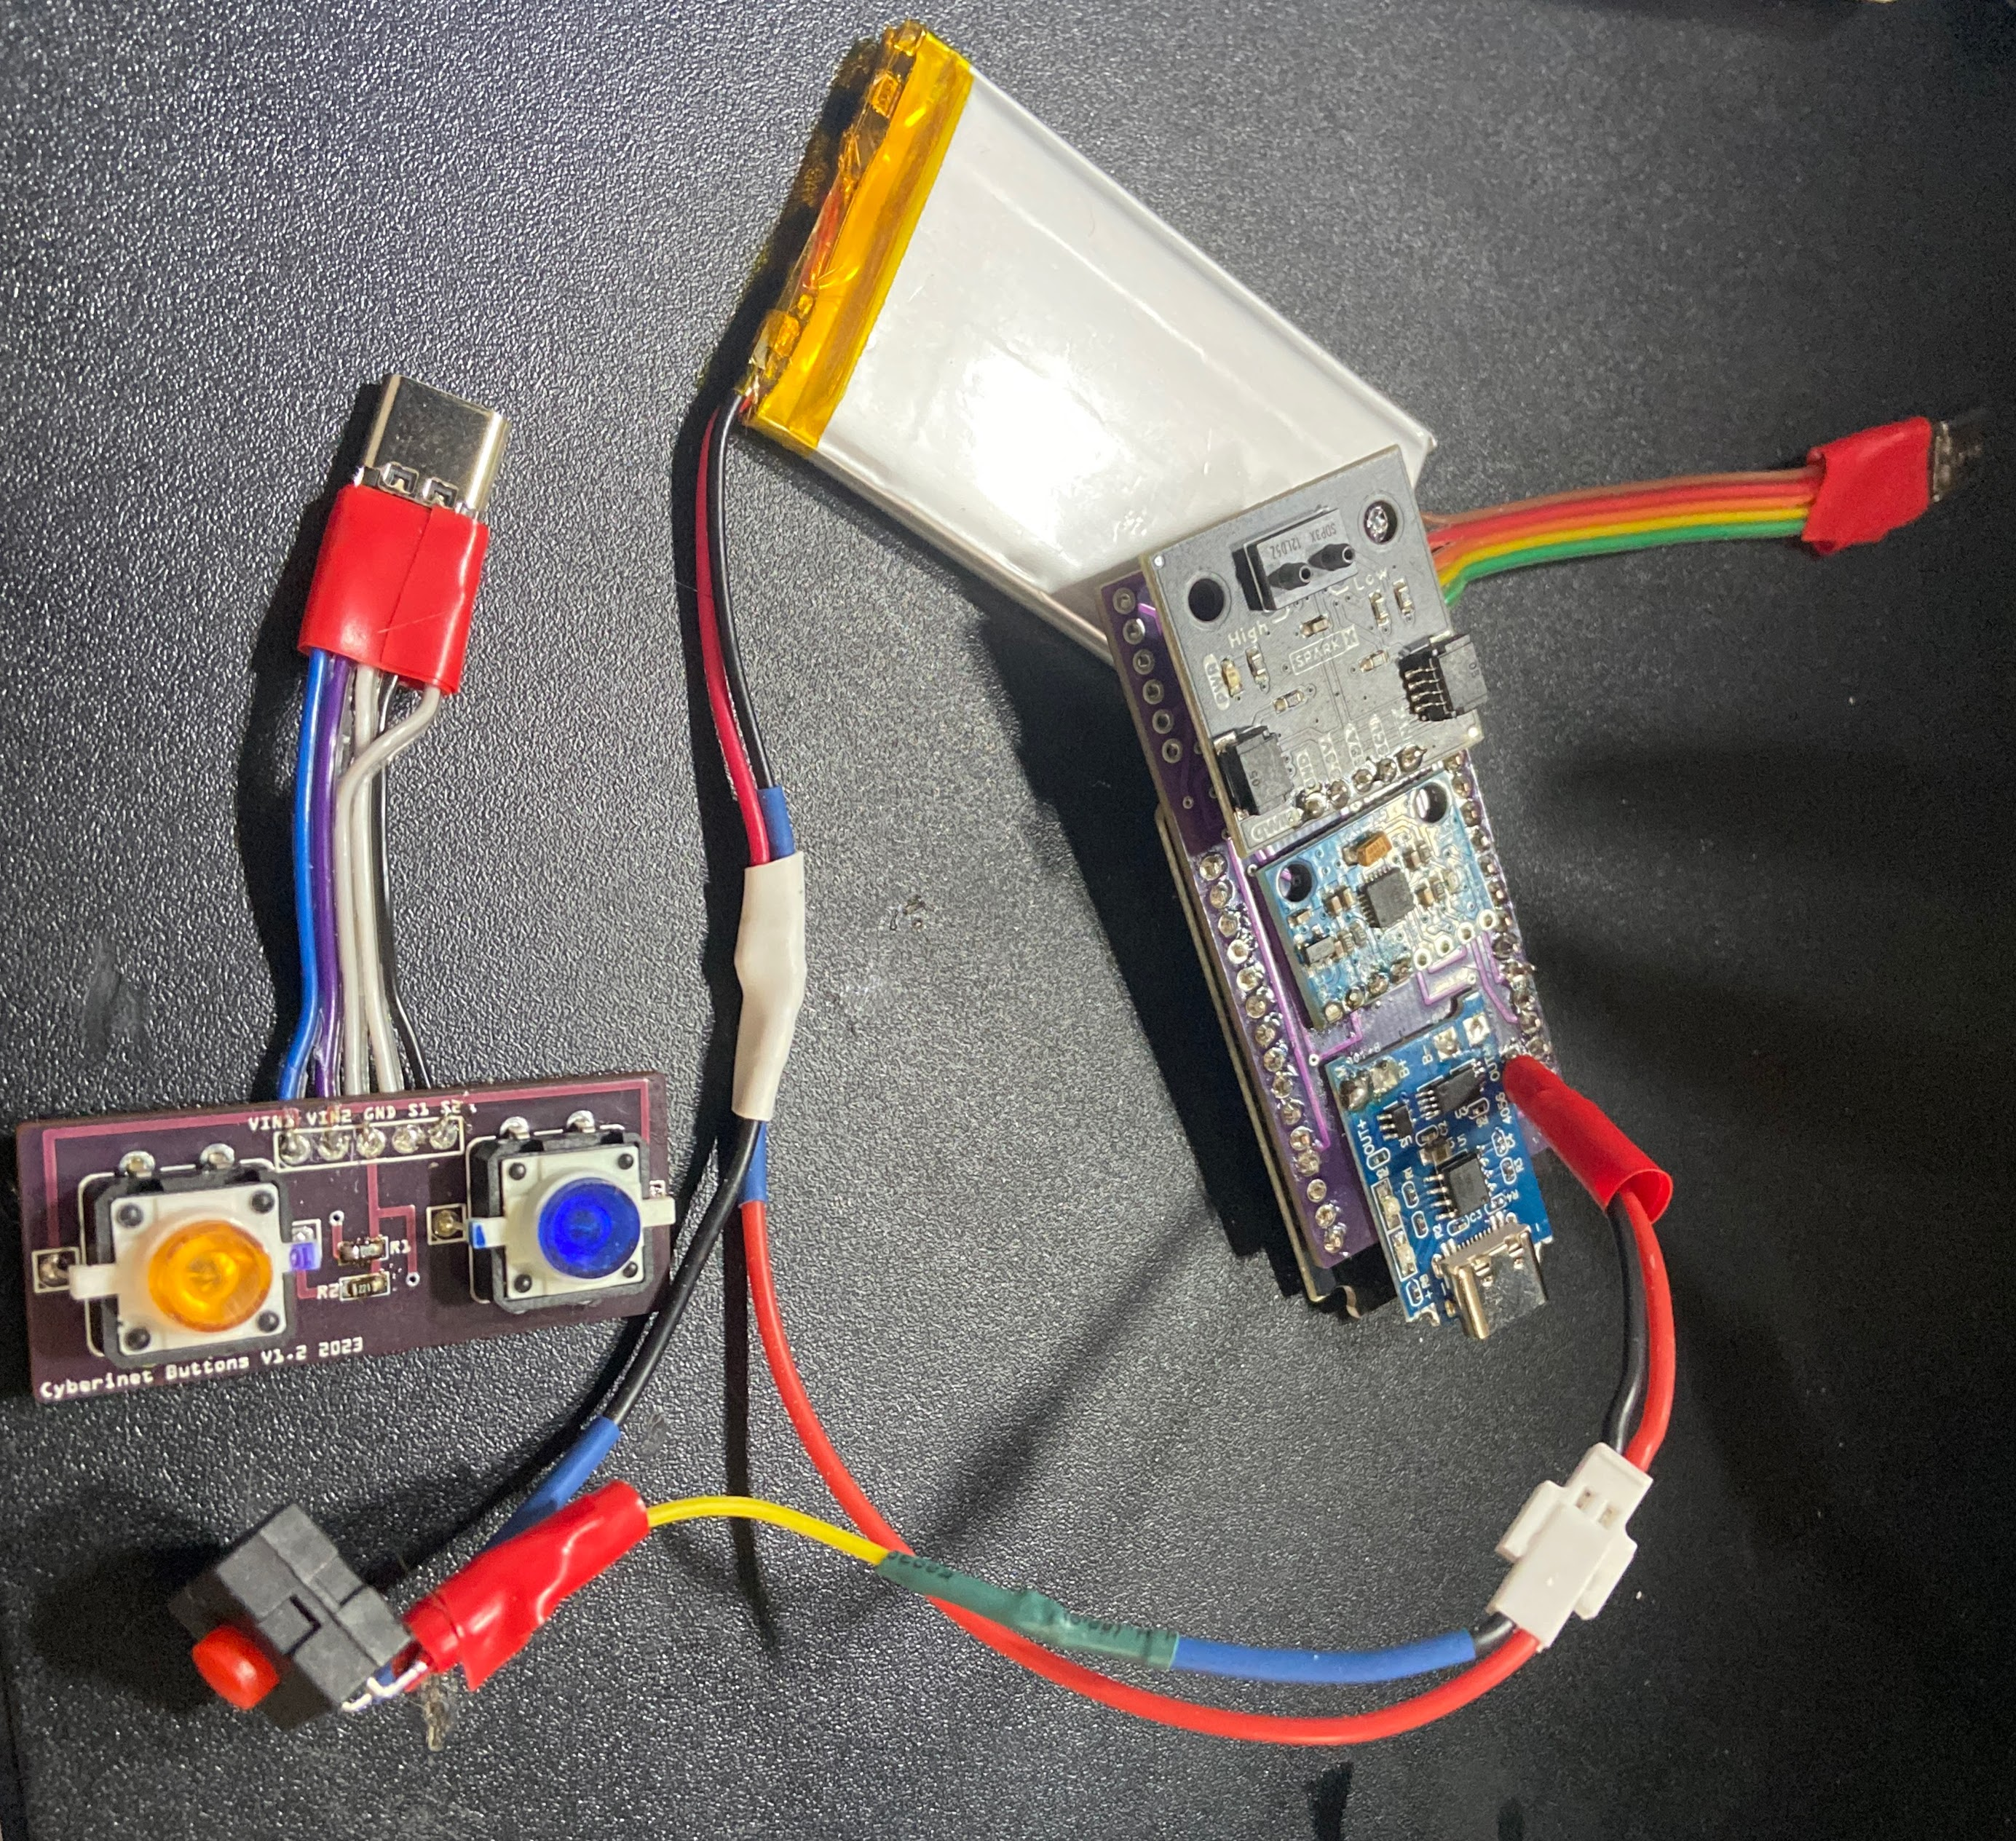
\includegraphics[scale=0.1, angle=90]{diagrams/builtUnits/noCase.JPG}
        \caption{Completed Cyberinet and Button Expansion without 3D printed housings}
        \label{fig:CyberinetNoCase}
    \end{figure}
\end{center}

When complete, the whole unit is slid into the 3D-printed case. Ports and tubes are aligned to the appropriate places and glued down to avoid unwanted movement. Not taking into account the space needed for the battery, tubing, and wired, the final Main PCB is approximately 5mm deep, creating a compact unit that can be easily placed in a variety of locations.

\begin{center}
    \begin{figure}
        \centering
        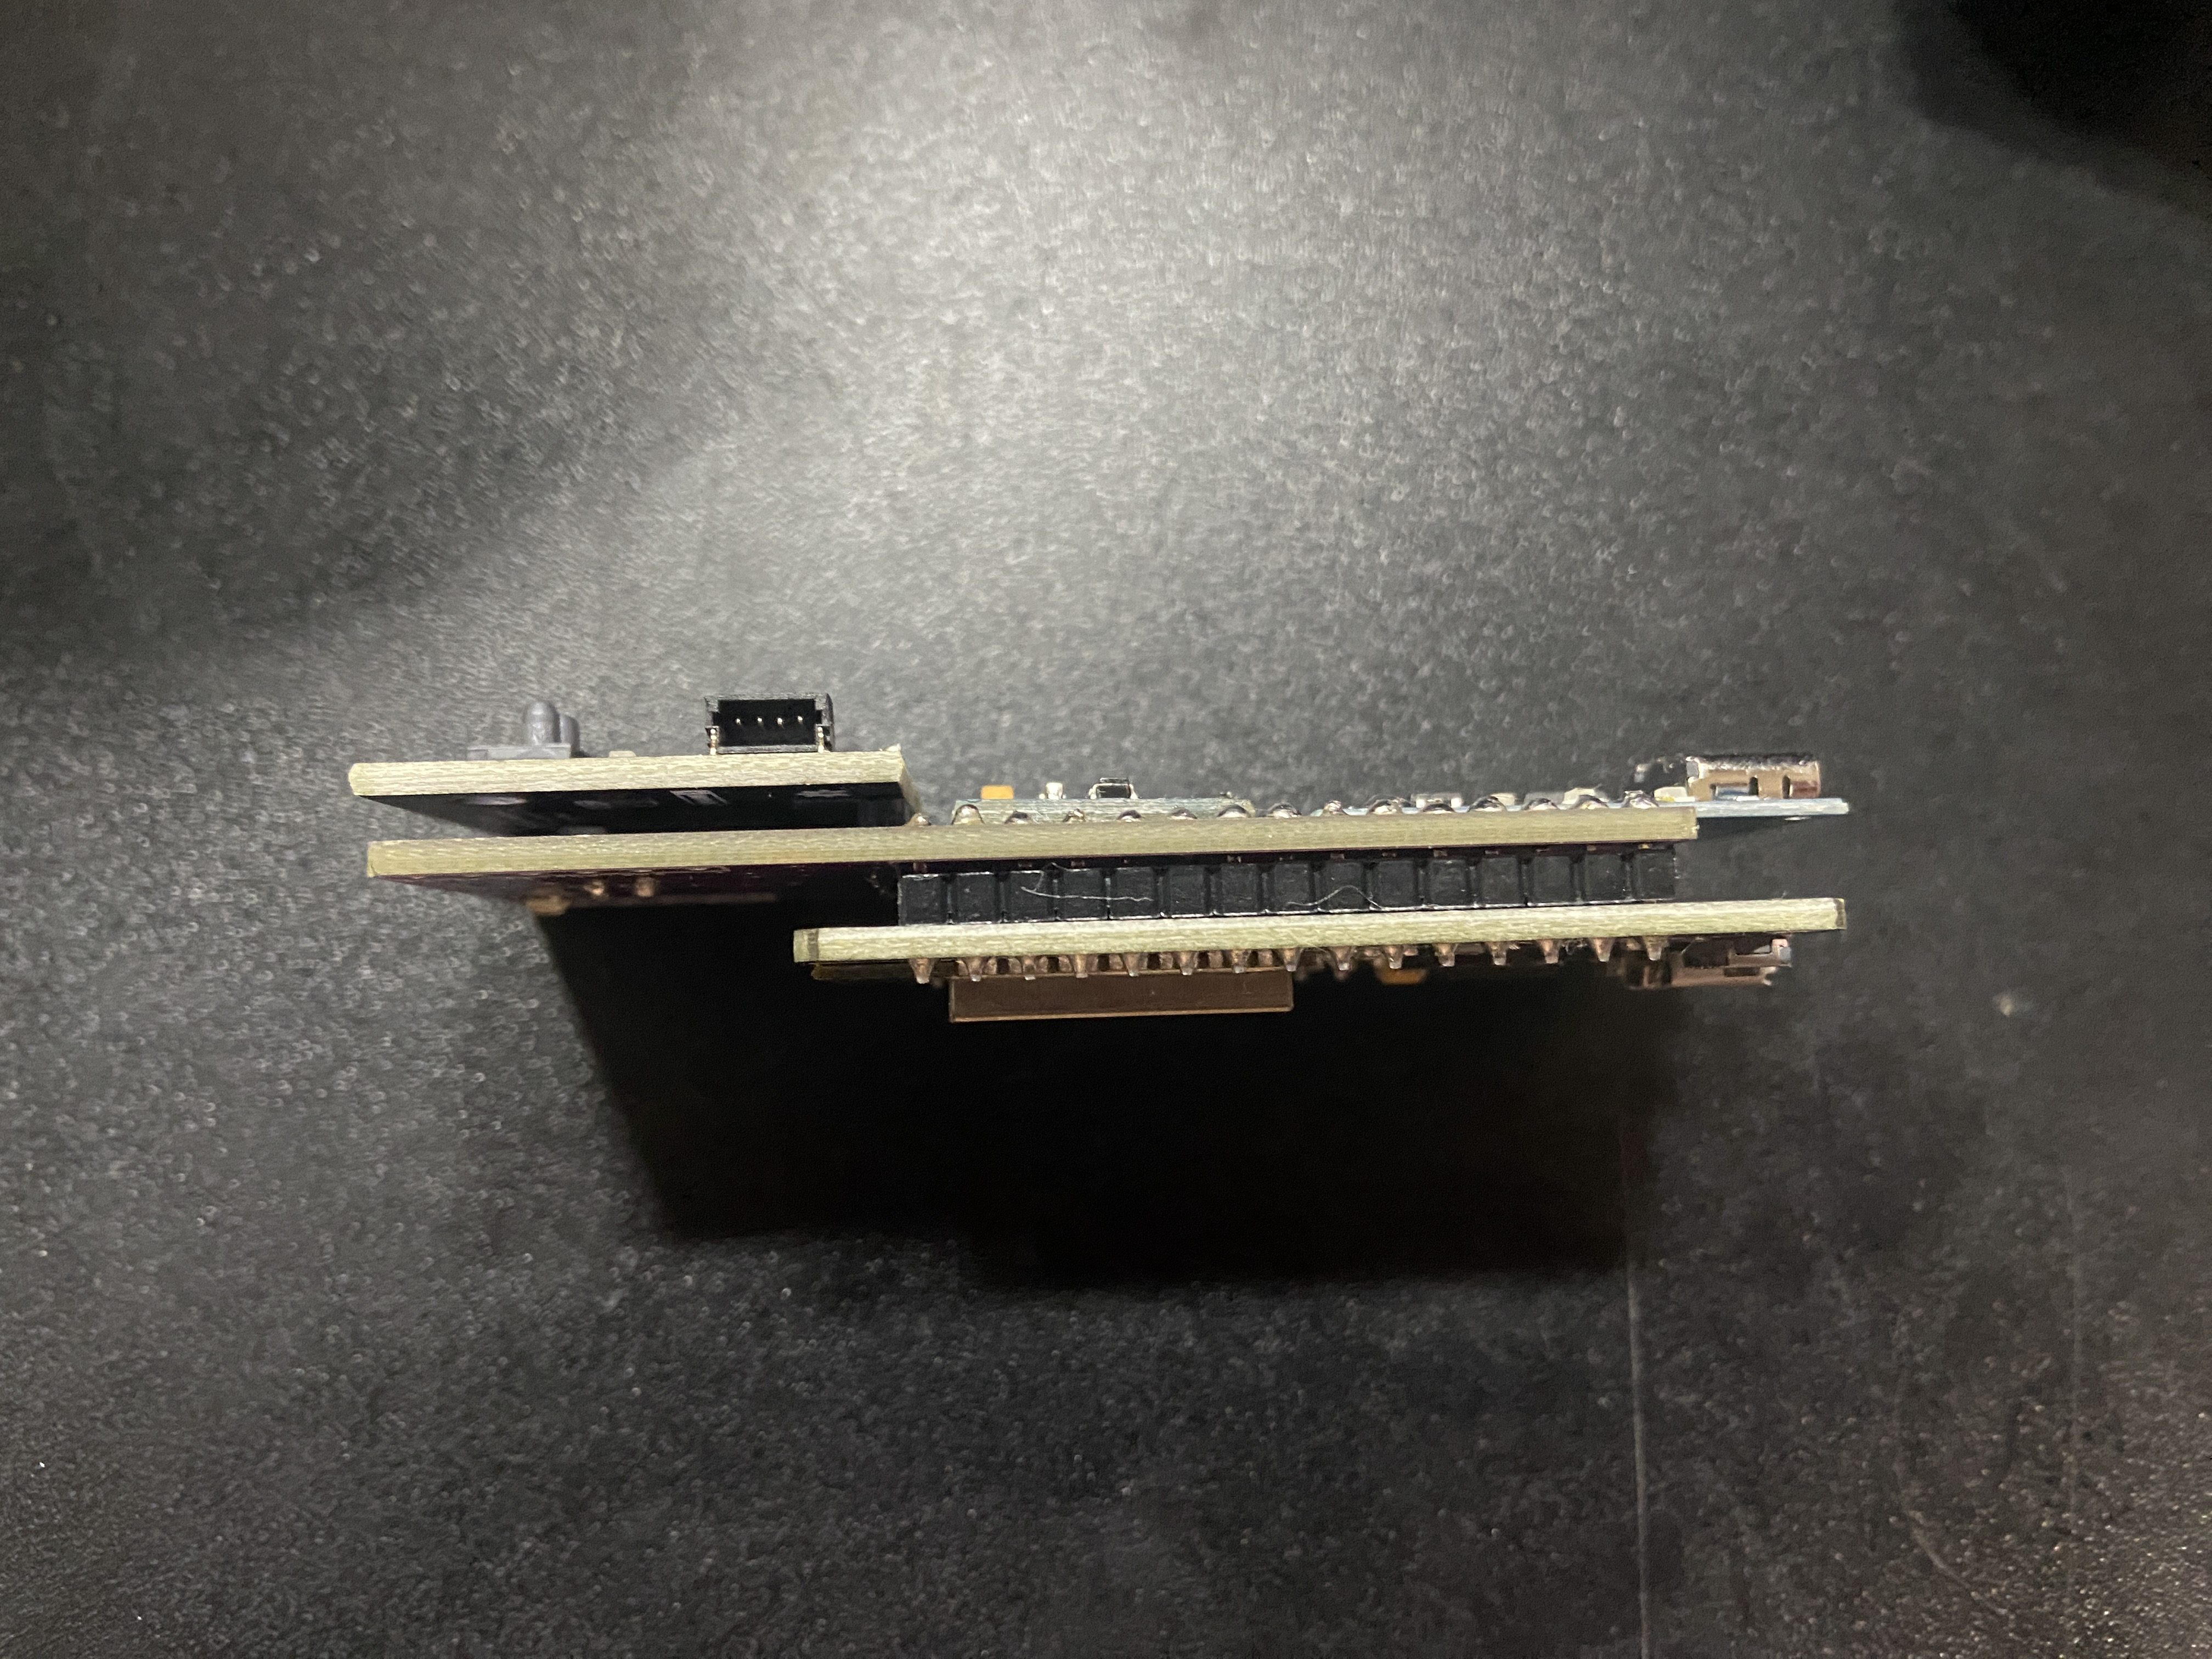
\includegraphics[scale=0.05]{diagrams/PCBs/cyberinetThin.JPG}
        \caption{Cyberinet Sensors Side View (No Casing or cables)}
        \label{fig:Cyberinetside}
    \end{figure}
\end{center}


Overall, placing the Main Unit's bulkiest components as close to the performer's mouth as possible results in the least amount of extra effort required to perform with the instrument. It is impossible to completely remove the added weight of the system additional, but this placement minimizes its impact on the performer.


\subsection{Expansion Assembly}

The Button Expansion is much simpler when compared to the main unit. The unit is composed of only two mechanical buttons with built in LED's, two resistors for those LED's, a USB-C port for communication with the Main Unit, a PCB to route all of the connections and the 3D printed housing. The button expansion is designed to be attached to the performer's thumb rest to allow for easy access with the right thumb. However it is also shaped in a way to allow for it to be held in the hand or placed elsewhere.

In the current software version, the button LED's are only illuminated when the buttons are pressed. However they are wired independently of the switches on the expansion. In future versions, the ability to control these LED's via the software is planned.

To assemble the unit, all components are soldered to the PCB. Like the Main Unit, SMD components are attached first, followed by cables, and finally the larger components. The completed PCB is then secured within the 3D-printed housing to complete the unit. The PCB for the Button Expansion is shown in figure \ref{fig:buttonPCB}, and the version containing all of the components soldered to it is part of figure \ref{fig:CyberinetNoCase}.


\begin{center}
    \begin{figure}
        \centering
        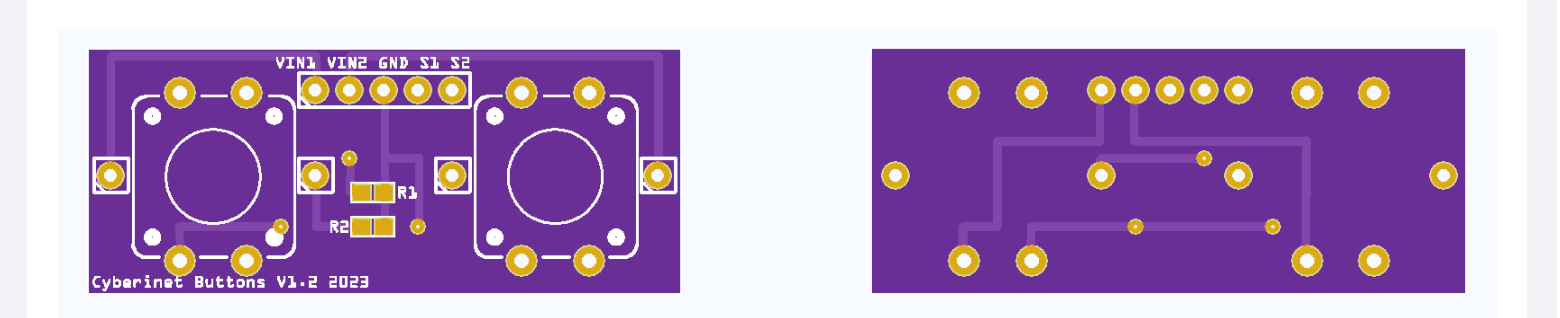
\includegraphics[scale=0.5]{diagrams/PCBs/buttons1.2.png}
        \caption{Button Expansion PCB}
        \label{fig:buttonPCB}
    \end{figure}
\end{center}


\section{Future Hardware Directions}
At the time of writing, the Cyberinet is only available for B-flat soprano clarinets. While this is the most commonly found Clarinet, it represents only a fraction of the total woodwind family. In the future, plans to adapt the hardware case to fit different instruments will allow for the Cyberinet to be utilized in an exponentially larger number of scenarios. 

First, adapting the unit for the A Clarinet and Bass Clarinets. At this time there are no plans to expand to an E-flat Clarinet due to the limited space to attach electronic components. Following the Clarinet expansions, ideas for compatibility with Saxophones and Flutes are being discussed, but require more planning in order to make functional units.

Outside of the aforementioned hardware needed to make the Cyberinet framework compatible with more instruments, improvements to the cable stress relief, and an increase in modular expansions is also planned. Initially only additional buttons available, but the aforementioned joystick and microphone expansions will be released over the summer of 2012. Additional plans for the following sensors to be released following those have also been made.

\begin{itemize}
    \item Pressure Sensor: responds to varying pressure on the instrument's keys. Needs special mounting of Force-Sensitive-Resistors, as well as doughnut-shaped FSRs.
    \item Pitch Detection: Works like the tuner software object. This will display tuning information and transmit pitch information to the computer. Needs hardware with adequate Analog-to-Digital Conversion.
\end{itemize}


\chapter{Programming \& Using the Cyberinet}
This chapter discusses the code located within the Cyberinet itself, as well as the accompanying library of Max tools. Discussion of the software portion of each of the included music compositions will be discussed in that chapter. In short, the Arduino code and the Max objects work together in order to achieve the four main steps in the functionality loop of the Cyberinet:

\begin{itemize}
    \item Step 1: Collect Data
    \item Step 2: Transmit Data
    \item Step 3: Receive Date
    \item Step 4: Route Data
\end{itemize}

\section{Arduino Code}
Another positive feature of the ESP-32 is that it is able to be programmed utilizing a variety of languages and environments. For the Cyberinet, the micro-controller was programmed using the Arduino coding language and Arduino IDE version 1.8\footnote{Arduino IDE Versions 2.0 and 2.1 were released during the Cyberinet's development, but were not utilized to avoid any compatibility issues during development. Future software versions will be created in more up-to-date IDEs.} This section will break down and discuss the components of the Cyberinet's on-board programming. The full .ino file's text can be found in this document's appendices.

\subsection{Collecting Data}
In order to collect the data from the sensors, each sensor has been given a function within the Arduino code. These functions serve the main focus of collecting and transmitting data. However because of the differing OEM sensors, each one utilizes a slightly different method of data collection and has a different range of values that can be expected. These functions are called in every loop of the program. Figure \ref{fig:getButtonsGetAir} shows the two most straightforward of these functions in their entirety.

\begin{center}
    \begin{figure}
        \centering
        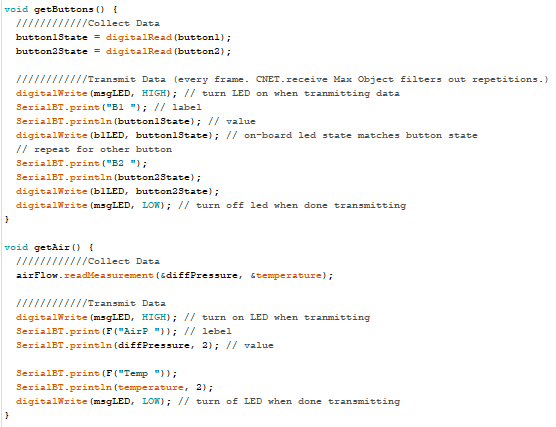
\includegraphics[scale=1.5]{diagrams/maxPatches/getbuttonsgetair.png}
        \caption{Cyberinet getButtons() \& getAir() functions.}
        \label{fig:getButtonsGetAir}
    \end{figure}
\end{center}

Looking at the function getButtons(), we can see the simplest of these functions. This function looks at pins 12 and 14 on the ESP-32, which are connected to the Button Expansion's USB-C connector. By utilizing the ESP-32's built-in pull-up resistors, the Button Expansion returns a 1 when the button is not being pressed and a 0 when the button has been detected as being clicked.

getAir() works in a similar function to getButtons(), but with a slightly different code because of the SDP-31's I2C connection and coding library. Because of this, the ESP-32 contacts the SDP-31 on its I2c address and requests the specific data at 2 registers. These data are labelled as 'diffPressure' and 'Temperature' respectively. 

The function 'get5060()' is shown in figure \ref{fig:get6050}, and contains a few more complicated steps than the previous functions. This function begins by communicating with the MPU-6050; essentially waking it up. Next, the data points for the gyroscope and accelerometer are requested. It is at this point that the function begins to differ from the previously mentioned ones.

\begin{center}
    \begin{figure}
        \centering
        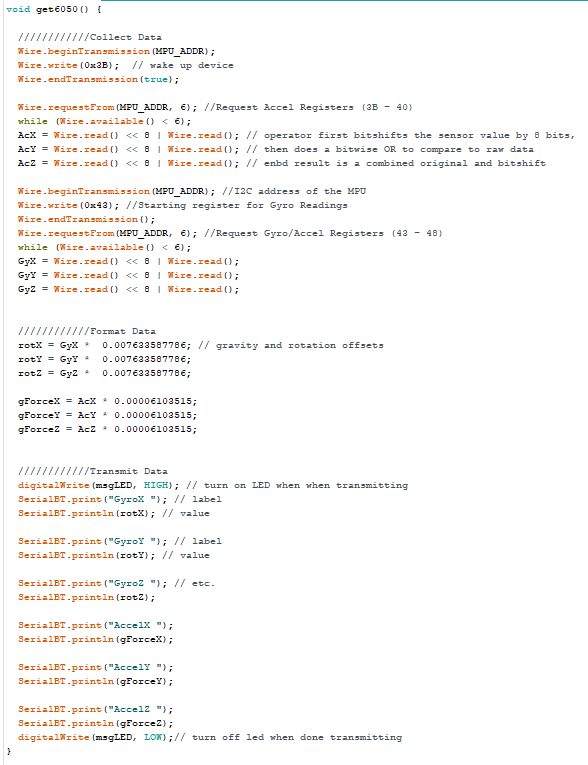
\includegraphics[scale=1.5]{diagrams/maxPatches/get6050.png}
        \caption{Cyberinet get6050() function.}
        \label{fig:get6050}
    \end{figure}
\end{center}

All six of the requested data points are then shifted over by 8 bits and then added to a second reading of the remaining data. This is done in order to fully read all 16 bits of data from the MPU-6050 on devices unable to access and process all 16 bits of data at once. 


\subsection{Transmitting Data}
The final portion of the data collection functions is the transmission of the data. This is done using the bluetoothSerial library, which allows for the ESP-32 to utilize serial communications over a Bluetooth connection. The .ino code's setup function is responsible for setting up these connections. The port is titled "CyberinetV13", indicating the version number with no spaces or punctuation, and utilizes a baud rate of 115200. This library contains the main Serial functionality present in Arduino, and simply is called with the instance name SerialBT to indicate the transmission is a wireless one.

Once all of the data is collected it is transmitted using the SerialBT.print() and SerialBT.println() commands. Utilizing the Max formatting, a label is created for each data point being transferred, then the individual value is transmitted, separated from the label with a space and ending with a carriage return. Each of the labels are listed in figure \ref{fig:sensorLAbels}. As briefly mentioned in Chapter 2, each sensor receives its own unique label. However, this is technically only true for the sensors present in the main unit. Because they share the same port and have a varying number of pins for returning data, the expansions all utilize the label 'exp' followed by the number. As mentioned previously, the expansion port contains six pins: power, ground, and four data return pins. Be keeping the data return format consistent between all expansions, it eliminates the need to identify the sensor in the moment. The main downside is that the user will have to remember what the sensor was in the programming environment, but this can be easily rectified with comments and notes.

\begin{figure}
    \centering
    \begin{itemize}
    \item gyroX
    \item gyroY
    \item gyroZ
    \item accelX
    \item accelY
    \item accelX
    \item airP
    \item temp
    \item b1
    \item b2
    \item exp1
    \item exp2
    \item exp3
    \item exp4
\end{itemize}
    \caption{Sensor labels used when transmitting data withe the Cyberinet}
    \label{fig:sensorLAbels}
\end{figure}

The data is sent in serial data packets, and the spaces and carriage returns are utilized by Max to help isolate the individual data and label values. The raw data stream as it appears in the Max console is shown below. To indicate that a data transmission has occurred, the red message LED is illuminated immediately before and toggled off immediately following the completion of the transmission. The end result is a rapid blinking of the red light when the Cyberinet is functioning properly. When combined with the green power indicator LED, the result can be perceived as a light changing between green and yellow through the holes in the 3D printed case.

% screenshot of the max console with all the values

The measured latency of the data transmission is measured at approximately % finish testing 

That value was repeatedly testing with the CNET.latency patch, which is discussed more in section 4.2.2. In order to arrive at the averages shown in figure % need to make figure with values after testing.
the test was repeated 10 times at 3 different distances from the control computer. 2 meters, 5 meters, and 10 meters were selected to represent a close, medium, and far distance while still remaining in the normal Bluetooth range\footnote{The current version of Bluetooth has a range of approximately 10 meters}.

CNET.latency can be utilized by anyone who needs to test the latency of their hardware unit. When loading the patch, and connecting the Cyberinet, a microphone and the button expansion are also needed. The user will place the microphone close to the buttons and press one of them which makes an audible click. This audible click is recorded, and then used to gate a small burst of white noise, which then is output from the speakers and picked up by the original microphone. Max then compares the number of milliseconds between the first button click and the burst of white noise from the speakers. This comparison calculates the full latency from an action on the Cyberinet to its result being herd by the user. The results of these tests are shown in figure  

\section{Max Programming}

To utilize the data being collected by the Cyberinet’s hardware, I have created a small library of Max objects to help with the collection and usage of said data. While detailed below, it is important to mention that Max is a paid software. The software and hardware components are all open source, however in order to create your own patches, the end-user will need to download the software. If saving patches is desired, then they must purchase a software license. Potential freeware options are being considered and will be explored upon more in a later chapter, but at the time of writing, are not in active development.

\subsection{Receiving \& Routing Data}

Once the serial data has been transmitted from the Cyberinet, it moves into the connected computer. This connection utilizes Bluetooth, and can be easily managed in the Max software\footnote{Max version 8.5 or newer is needed when working with the Cyberinet}. A single object is utilize in order to help receive and parse the data stream from the Cyberinet. CNET.receive allows the user to easily determine which Bluetooth port to receive data from, then sends it to various object outputs for use in the Max environment.

% picture of inner workings of CNET.receive
% \begin{center}
%     \begin{figure}
%         \centering
%         \includegraphics{}
%         \caption{Caption}
%         \label{fig:my_label}
%     \end{figure}
% \end{center}

In short, this Max object runs a small Node script that helps to import the data into Max. This script specifies the desired serial port, then using the space and carriage return characters, formats the data into the label and value pairs that Max expects. These values are then routed to individual outlets based on their labels\footnote{Each outlet is given a label so that the user can identify what the numbers leaving the object are}. Prior to leaving the outlets, the data is then scaled to fit a range of 0-1. This helps to keep all of the sensors within an easily adjustable range for other objects within Max. The only exceptions to this are the buttons which only output 0 or 1 when the button state changes, and the temperature which is measured in degrees Celsius and not scaled at all. 

In order to utilize this object, you must first connect the Cyberinet to the computer via Bluetooth. after the connection has been established, sending a bang into the first inlet will open communications on the default port. If the desired port is not the default, then sending the message "setPort" followed by the port name will change this. From there data will begin automatically flowing through the patch to the desired outputs. If you wish to see the raw, un-scaled data in the Max console, toggle the second inlet on. A bang to inlet three will stop communications, and a bang to inlet four will install appropriate NODE drivers and dependencies to allow Max to utilize the javascript code. This is only required one time on each computer.

\subsection{CNET Objects}

While not necessary for the functionality of the Cyberinet, I have also created a small collection of Max objects for use with the unit. These objects were all used within the Compositions discussed in chapter 5. All of these objects are designed from the ground up to receive data from the Cyberinet in order to control their functionality. These include:

\begin{itemize}
    \item reverb~: a Schroder style reverb based on examples from CCRMA.
    \item compressor~: Based on the compressor objects created by Cycling74.
    \item delay~: A single delay line using the tapin~ and tapout~ objects. 
    \item MultiDel~: A delay line utilizing 4 different tapout~ objects to create multiple delay lines. Each one can have its individual output level set for unique mixing capabilities.
    \item feedbackDelay!: Identical to the simple delay, but with a feedback option added.
    \item vibDelay!: Functions similar to the Simple delay object, but includes a basic implementation of FM synthesis to adjust the pitch of the signal to be delayed. 
    \item tuner: This object functions like most other tuners available on the market. It will determine the pitch of an incoming signal and output the value as a signal. This is useful for checking and maintaining tuning within the Max environment, and for having the Max patch respond to certain pitches. This object requires a microphone be used to monitor the input as the ADC capabilities of the ESP-32 DEVKIT are unable to pull off this effect.
    \item pitchShift~: changes the pitch of an incoming signal. This can be controlled by MIDI  numbers or the 0-1 floating point range of the Cyberinet. The values input here are the desired pitch of the signal, not the amount by which it is shifted. both his and CNET.tuner also have a dry digital pass-through and latency monitor,
    \item latency: Designed to test the latency of the Cyberinet within  the Max environment.
\end{itemize}

In addition to the above objects, the Cyberinet software also includes a few objects intended to be helpful in setting up and trouble shooting. The main one of these objects is the tuner object. This object serves as a tuner within the Max environment, allowing for quick adjustments to be made without needing an additional piece of hardware. 
The main downside to the tuner object is that it requires the use of a microphone input to the computer. This is due to the limited ADC capabilities on the Cyberinet's main ESP-32 Board. However, an unexpected upside to the object is it's pitch detection capabilities. The tuner object is able to detect both the musical pitch of the incoming signal, but also fine tuning in cents. Because this information is expressed in MIDI, it can be used to trigger a variety of other events in the max environment. While the list of possibilities is extensive, the idea of having the max patch harmonize with the clarinet is one of particular interest to the author.

\subsubsection{Help \& Tutorial Patches}
The final software element of the Cyberinet is the implementation of Max help patches. These patches provide relevant documentation for each of the objects mentioned both in this chapter and Appendix B. They also provide a short tutorial for how to utilize the object both with and without the Cyberinet hardware. 

These help patches describe what each effect does, and breaks down what each inlet for the CNET objects controls, the data ranges, and default values. Each help patch also includes three or more presets that show off a variety of different 


\subsection{}section{Future Software Directions}
Lastly, Plans for the expansion and revision of the software environment are already underway. Future goals include:
\begin{itemize}
    \item Adapt messages to OSC formatting for a greater range of software compatibility.
    \item OS compatibility: Version one of  the Cyberinet currently only works on MacOS devices. Future plans involve compatibility with Windows devices as well.
    \item Increasing Effects: Expanding for additional audio effects. Plans include filters, synthesizers, and automatic harmonizers.
    \item Max Library: Once expanded and revised, Plans to reach out to Cycling74 to have this collection of Max objects listed in the program as an available-for-download library will be made. This will make it simpler for people to access various tools for their Cyberinet unit.
    \item Standalone Software: The final planned software expansion for version one is to take the Max environment and export it as a standalone software. This will allow for the user to access the tools and capabilities of the Cyberinet without needing Max, which can be a financial hindrance to some people.
\end{itemize}

\section{Mapping Gestures to Max} %if super long, may need to make into a seperate chapter.

The idea of mapping physical gestures to the sound production/processing created by an augmented has already come up a few times. While indeed this can be done haphazardly or randomly, in order to properly utilize the cybernetic capabilities of the Cyberinet (or any other digital musical instrument), the performer must be able to respond to the current state they are in and create either a positive or negative feedback loop to maintain, grow, or diminish the current state. In order to do this, it is important to identify gestures being used and how they are mapped. This section will go over various common gestures created when performing naturally on the clarinet as well as experimental gestures that can be used to explore various effects. We will then explore the data related to these gestures, and in the following chapter, how that gesture data can be applied in various settings.

\subsection{Commonplace Gestures}
All of the gestures discussed here are ones found commonly in clarinet performances. It is by no means an exhaustive list, but serves to act a s a general outline to the more common movements I have either done as a clarinetist, or seen done in many performances. If heavily exaggerated, each of these movements could easily be defined as more experimental

\subsubsection{Fast upward, then hold}


\subsubsection{Circular motion}



\subsubsection{Swaying}



\subsubsection{Close to body, minimal movement}



\subsubsection{High angle}




\subsection{Experimental Gestures}



\subsubsection{Movement, no playing}



\subsubsection{Spinning}



\subsubsection{Inhaling through instrument}







\chapter{Intended Uses}
Now that we have looked into aspects of augmented instruments and cybernetic music, let us take a moment to see how they apply to the Cyberinet and the device's intended uses before we dive into the creation of and working with the Cyberinet.

While adaptable, the Cyberinet was envisioned with a handful of specific uses in mind. As is, the Cyberinet is intended to be an easily-removable add-on for a standard B-flat clarinet. This add on allows for the user to easily include computer augmentation into their timbre repertoire. 

\section{Composition Tool}
One of the three main intended uses of the Cyberinet is as a compositional tool. Effectively, treating the Cyberinet as a completely new instrument or an add-on to a traditional B-flat clarinet. The flexibility of utilizing the Cyberinet's sensor data can result in a large variety of potential sounds, even without the need for the clarinet to make sounds. A performer can utilize multiple Cyberinet sensors without traditionally playing the instrument, allowing the composer to explore new performance routes.

The cybernetic capabilities of the Cyberinet also allow for experimentation with the interplay between the acoustic performance and the electronic components. The modularity of the sensor routing within Max and the choice of expansion sensors also help to increase the creative sound possibilities.\footnote{Early versions of the Cyberinet are intended to focus more on the alteration of the clarinet sound and controlling the Max environment, but more experimental developments are planned following the initial release.} The compositions discussed in Chapter 5 all focus on the variety of creative possibilities with the Cyberinet. 

Discussed in more detail in Chapter 5, each composition features a different utilization of the sensors. \textit{Puzzle of a Park} utilizes the button expansion to control a Max patch. The end result is similar to a loop pedal. \textit{Ethereal Presence} utilizes accelerometer data to control harmonization and backing noise. \textit{Raindrops on a Tin Roof} utilizes all of the available sensors in version 1.3 to trigger sound file play back, processing of live and recorded sounds, and live lighting changes.

When mapping the gesture data, a composer is able to define specific movements to occur at specific moments within a performance. However, as explained by Kvifte and Jensenius, it is important to consider the perspective of the listener\cite{KvifteJenseniusDescription}. From this perspective, the listener will identify a gesture and the resultant musical sound. This will happen regardless of if the identifies gestures are actually creating the sound. in a 2005 study, Wanderley et. al have found that:

\begin{quote}
    ... clarinetists' ancillary gestures are not randomly produced or just a visual effect, but rather they are an integral part of the performance process\cite{wanderleyClarinetGesture2005}.
\end{quote}

The Cyberinet functions by taking these generally ancillary gestures, and translate them into the realm of audibility. In order to translate this clearly, the parameters must be clearly described to the performer with a much greater level of specificity than would be needed than if describing it to a listener\cite{KvifteJenseniusDescription}. Using Kvifte and Jensenius' paper as a methodology for describing these gestures again, The Cyberinet exists squarely within the ratio level of measurement. This level of data is measured, with the distance of values determined, and an absolute zero value for each data exists, allowing for there to be 0 movement or airflow in the system. Being composed of specific values between 0 and 1, the data collected from the Cyberinet serves as a discrete input to the Max objects. Because of the modularity in the output, the sound production can be either continuous or discrete.

In practice, this results in a need for specificity in gesture notation to fully take advantage of the Cyberinet. A score needs to explain what, how, and when to perform certain gestures like those indicated within the previous chapter, as well as what the intended effect is\footnote{Chapter 5 will discuss how this was done or intentionally avoided, and how effective this was in practice.}. Mappings can be static, where a gesture will remain fixed to a specific parameter. Variable mappings can be changed by the performer either as instructed or in a improvisation manner. Another option discussed by Kvifte and Jensenius is the system being able to learn and modify itself based on the gestures of the performer\cite{KvifteJenseniusDescription}. While highly cybernetic in concept, the works discussed in Chapter 5 do not utilize this method of mapping.

As a final note on specifying the gesture mapping, It is recommended to avoid mapping multiple gestures and sensors to a single effect at one time. This can easily obscure what the listener is perceiving as the gesture, leading to an ambiguous relationship. However, having multiple effects controlled by a single gesture is less problematic as it can create a more complex musical result to an initial gesture.


\section{New Instrument}

As mentioned, the Cyberinet is intended as a new tool for the composer, but what about the performer? The Cyberinet straddles a line between new and old. It works to bring new sounds and functionality to a traditional instrument with its own performance practice. While the initial performances of the Cyberinet are intended to straddle this line, that is not all it can be. My ultimate goal is to treat the Cyberinet as its own unique instrument. Speaking purely practically, this brings about a certain mindset in the composer and performer when creating new music. I want the users to create music with the electronic features in mind, rather than working for an acoustic clarinet with additional aspects added. In writing the original compositions, the allowed for a more intentional integration of the motion and breath sensors, which resulted in clearer, more dramatic effects in performance.

As mentioned by Reid in regards to the MIGSI trumpet, creating a new computer-augmented instrument brings various elements to the forefront of the creation procession that would not normally be of concern. Specifically latency\cite{reid_2019}. When designing the Cyberinet, it was necessary to separate the instant audio response of the clarinet base from the electronic sound alterations and productions, which have a comparatively large amount of latency. The specific patch and process used to calculate latency is discussed in Chapter 3, and the measured average latency of the Cyberinet is PUT TIME IN HERE.

\section{Improvisation Tool}
% a la stomp boxes
Straddling the line between composer and performer brings us to the final, performance-based intended use for the Cyberinet: an improvisation tool. While mainly intended as a compositional tool, the Cyberinet leads to a large amount of exploration and improvisation. A few audio effects are provided with the Cyberinet to allow for the user to easily begin creating their own sounds, however the system can easily send its data to any object within the Max environment. By exploring which sensors are connected to different audio effects, the performer can create a large number of sounds based on a single performance movement that they are already used to. The large variety of options are discussed earlier in this chapter.

This modularity in signal processing is similar to the practice of using guitar stomp boxes to make a unique sound. While not physically similar, both systems allow for the quick customizable alteration of the instrument sound. When designing the available software objects, effects present in effect pedals such as reverb, delay, filters, and tuners were used as an inspiration. From a pure performance standpoint, the Cyberinet can be utilized to significantly reduce the amount of equipment needed. The goal of this is to free up the performer and allow them to be able to improvise and create new sounds more freely, without the need to consciously manage equipment.

\section{Educational Tool}
Admittedly, at the time of writing the idea of utilizing the Cyberinet as an educational tool is the least concretely defined idea discussed in this chapter. The concept came about when discussing the Cyberinet with various performers and graduate students during the LSU 2023 College of Music \& Dramatic Arts Research Expo. While not initially conceived in this manner, I feel that implementing the Cyberinet as an educational tool can have interesting and long-reaching results for future clarinetists and electro-acoustic music performances. 

In short, these discussions focused on the gyroscope (MPU-6050) and differential airflow pressure (SDP-31) embedded sensors. Looking at the gyroscope, the ability to determine the instrument's position could prove useful for new students learning the correct performance posture. This was the consensus of the small group of graduate researchers at the aforementioned event. I felt that bringing up the gyroscope in early education may have a unique side effect that was not brought up in the casual discussion, that being a potential to apply Cybernetic or Deep Listening concepts to a performer's mindset from an early age.

If a performer is able to see clearly on a screen what their current position is and how to change that to improve their sound and posture, then they are learning how to observe and analyze their body and make changes to the system in real-time; creating a Cybernetic feedback loop\cite{WeinerCybernetics2019}. While beyond the scope of this document, this action brings to mind several concepts of the Alexander Technique\footnote{For more information on the principals of the Alexander Technique, visit \url{alexandertechnique.com}}. Specifically, the concept of self-awareness and adjustments to free the performer from habitual problems\cite{gelbBodyLearning2013}.

It was with this context of seeing and learning to be aware of the air pressure that the conversation led into the use of the SDP-31 in an educational sense. By giving real-time numerical feedback a performer could learn what values to expect when performing at various volumes, the maximum and minimum amount of pressure difference they are able to create, as well as potentially identify any potential holes in their embouchure or leaky pads on their instrument. The same level of Cybernetic awareness and feedback apply to this sensor as well.

As additional expansions are created for the Cyberinet, their potential use in a pedagogical environment will need to be evaluated. Several of the expansions discussed in Chapter 2 have potential for educational use, and more could be created following appropriate design and market research.

\chapter{Music Works Written for the Cyberinet}

In addition to creating the hardware and software for this dissertation, I have also created a handful of musical compositions that show off various features of the Cyberinet. These three compositions as listed below, show a gradient from simpler to more complex uses of the Cyberinet’s features.

Before we begin looking at the compositions in detail, I want to explore what it is like performing with the Cyberinet through an interview with the premiere artist for all three of the works mentioned in this chapter\footnote{The scores for all pieces discussed in this chapter are available in the appendices and online at \url{matthewbardin.com}}.


\section{Puzzle of a Park}
At its core, this work is the simplest of the three written especially for this project. \textit{Puzzle of a Park} functions as a work written for a loop pedal, but without the pedal. The performer plays through the material from beginning to end, periodically pressing one of the two buttons on the button board accessory. Looking at the max patch we can see that one button will trigger the computer to record a microphone input into a buffer while the second triggers the synchronized playback of all recorded buffers. 

%[show patch snapshot]
\begin{figure}
    \centering
    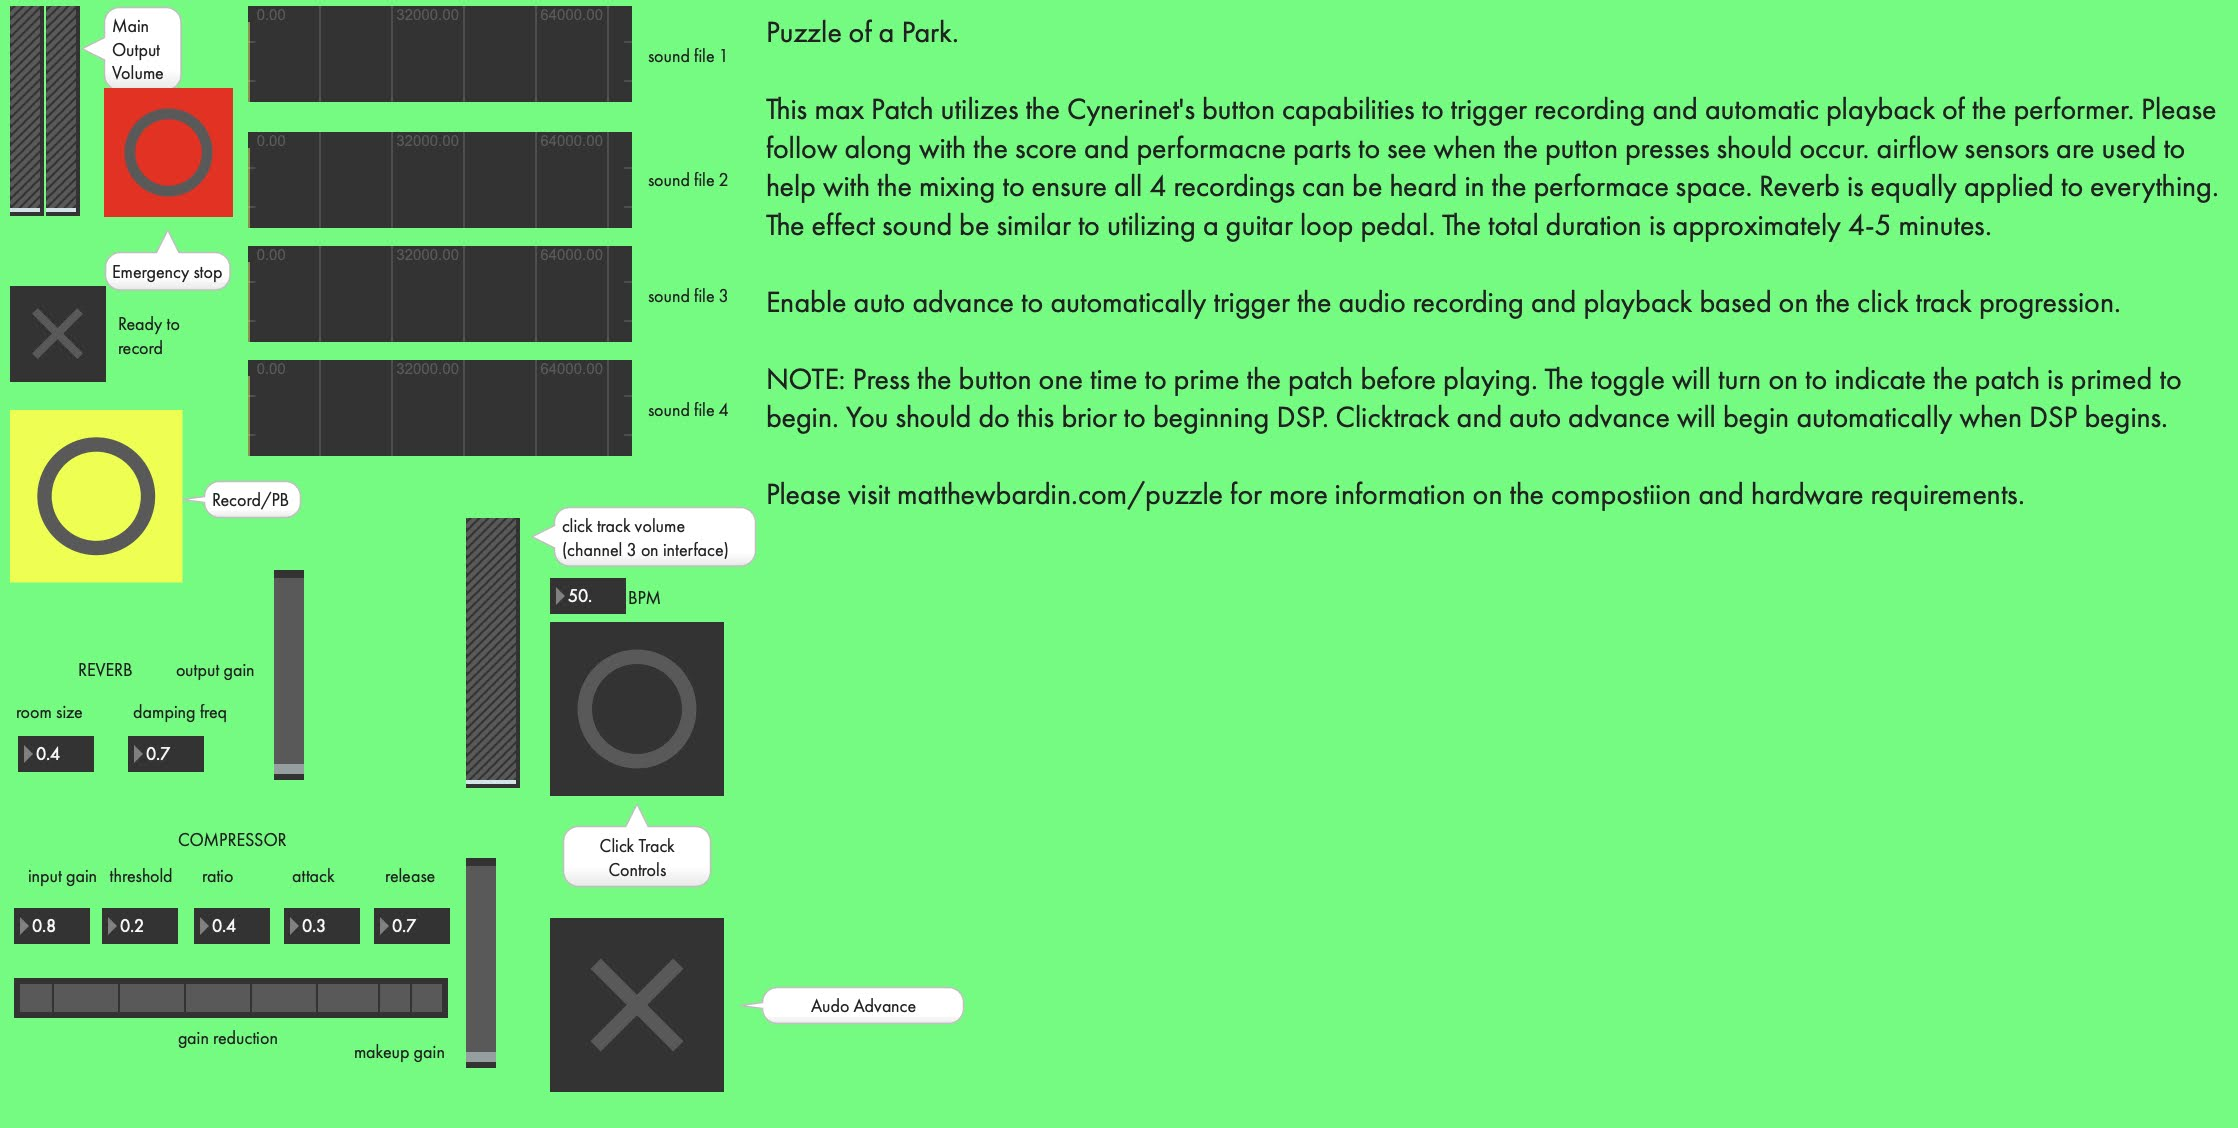
\includegraphics[scale=0.2]{diagrams/maxPatches/puzzlePresentation.jpg}
    \caption{\textit{Puzzle of a Park} Max Patch Performer View}
    \label{fig:puzzlePatchPres}
\end{figure}

\begin{figure}
    \centering
    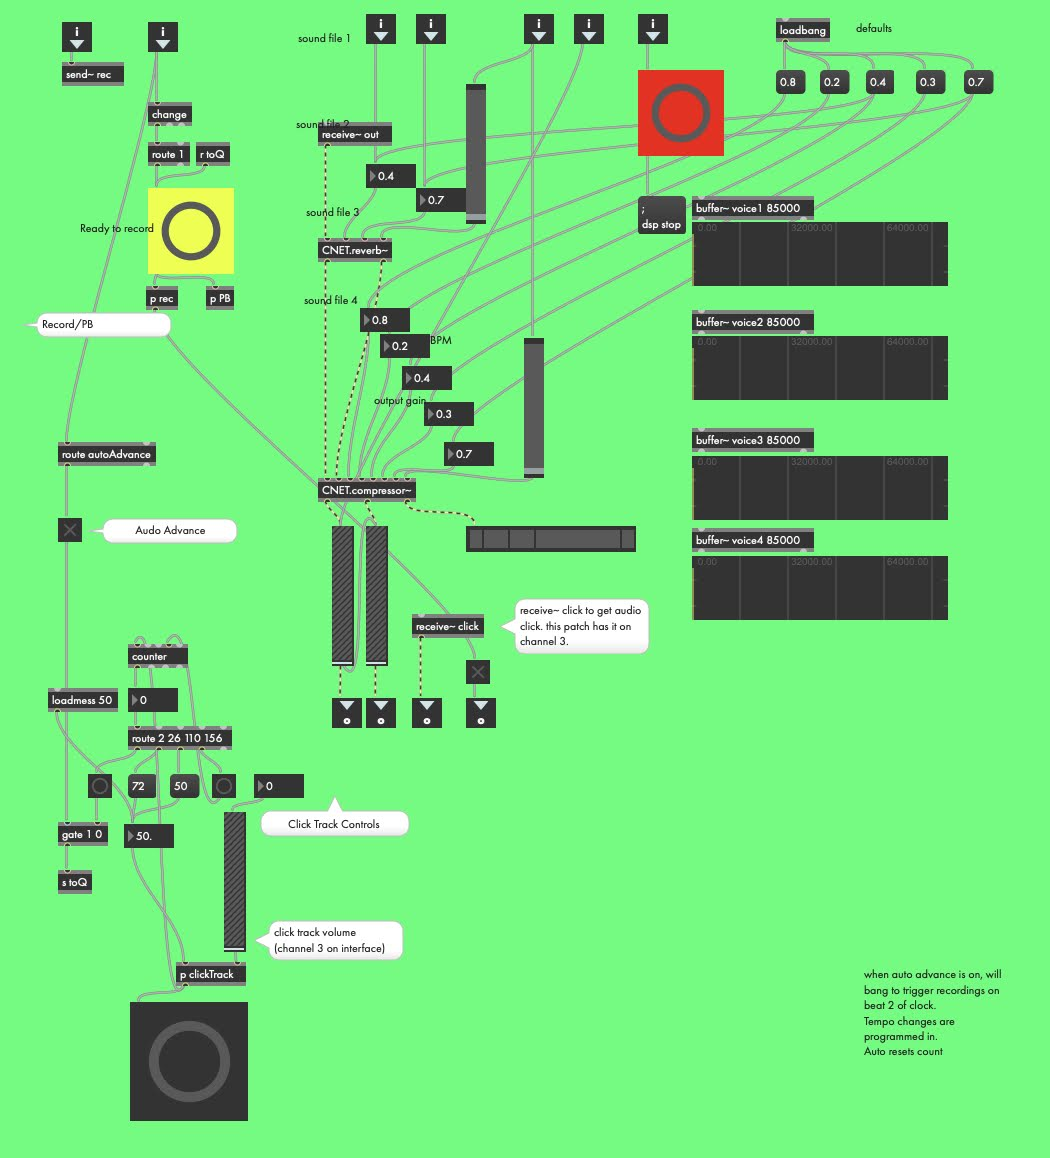
\includegraphics[scale=0.25]{diagrams/maxPatches/puzzleRaw.jpg}
    \caption{\textit{Puzzle of a Park} Max Patch Full View}
    \label{fig:puzzlePatchRaw}
\end{figure}

This functionality allows for multiple recordings to be saved and layered, much like loop pedals such as the Boss RC line of pedals.

When writing this work, I viewed the musical content as a quartet, with four unique voices rather than a single voice repeated several times. This allowed the musical content to flow and feel more organic once the final layer was added. 
Once I had completed the short musical section, it was simply a matter of repeating the sequence of time signature and meter changes so that the score would form a repeating pattern. From there I had to decide exactly how to organize the sounds in time. Because I wanted this to be the simplest of the works in terms of performance and programming, I refrained from breaking down the recordings into smaller chunks and assembling them in Max. Instead, I choose the loop pedal approach and had the performer play through each voice before starting the playback and recording for the following voice. 

When ordering the voices, I began with one of the middle voices as the opening to the solo part. When comparing the voices in the score, these helped to provide a large amount of the background and a steady, albeit syncopated, pulse to the music. Something that helps to give the following bass voice more context during the measures where it is simply holding a pedal tone during the second section. Looking at the large-scale musical form of the solo, I would describe it as \emph{ABA'C} since the third and first voice are often coordinated, providing harmonic content. I viewed them like a horn part in a Sousa march in this regard. When combined, the first three voices provide a complete backing track to the main melodic line. Like fitting together, the pieces of a puzzle, it is this final line that helps to give context to all the phrases we have heard so far. Down beats become upbeats, harmonic implications shift with the addition of new chord tones, and the texture is filled out to include the full range of the instrument.

\textit{Puzzle of a Park} was premiered by Adam Cope on 04/18/23 at the LSU Digital Media Center Theatre

\section{Ethereal Presence}
The second work\footnote{A performance video of \textit{Ethereal Presence} is available at} created for this project begins to utilize the more complicated sensors present in the Cyberinet. These primarily include the gyroscope and airflow meter. Once received, the Max patch for the composition utilizes the values to control two different synthesizers and their parameters, listed in figure \ref{fig:etherealSynths}. 

\begin{figure}
    \centering
\begin{itemize}
    \item Pitch-shifted triangle waves that harmonize with the original clarinet sound.
    \item Filtered pink noise using FFT bins that respond to the position of the performer.
\end{itemize}
    \caption{Synthesizers used in Ethereal Presence}
    \label{fig:etherealSynths}
\end{figure}



The first synthesizer outputs three triangle waves with the goal of harmonizing with the soloist. This is the Ethereal Presence as mentioned in the title. The goal is to make the tone as simple as possible, but with a large potential for timbral changes. The pitch of the incoming microphone signal is analyzed using CNET.tuner~, which is used to determine the pitch of the three triangle wave oscillators. All three can have the specific harmonization change with the sensors input, but one is scaled to always be below the main pitch, another is relatively close to the main pitch, and the third will always be higher. The result is a chord that both matches with the incoming pitch, and can morph based on the performer's position or dynamics. 


Accompanied by this is a more textural synthesizer designed to help support and fill out the atmosphere of the composition. This synthesizer outputs noise before being run through an FFT, based filter created by Dr. Austin Franklin. This filter takes the incoming noise and performs an FFT operation on it to determine the frequency content, then based on the values received from the Cyberinet, filters out certain frequency bins. The end result is a fluctuating cloud of noise that adapts its frequency range based on the Cyberinet's position.


\begin{figure}
    \centering
    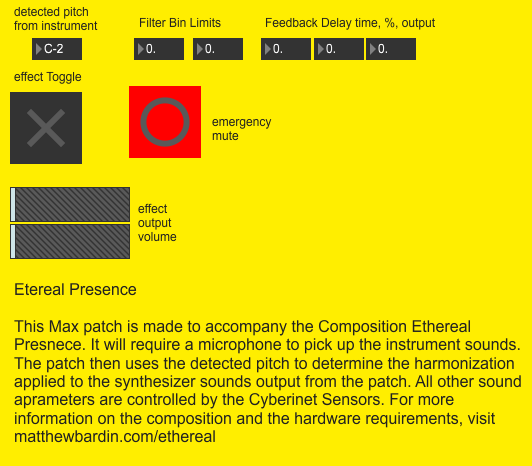
\includegraphics{diagrams/maxPatches/ethereal_pres.png}
    \caption{Ethereal Presence Performer View}
    \label{fig:etherealPerf}
\end{figure}

\begin{figure}
    \centering
    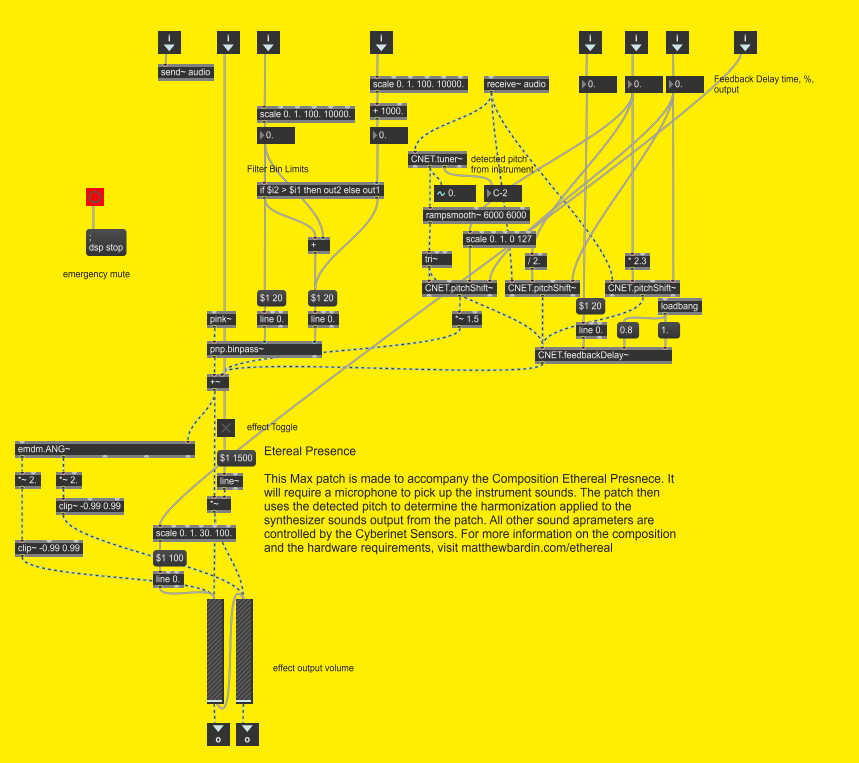
\includegraphics[scale=0.75]{diagrams/maxPatches/ethereal_raw.png}
    \caption{Ethereal Presence Full View}
    \label{fig:etherealRaw}
\end{figure}


\textit{Ethereal Presence} was premiered by Adam Cope on 04/18/23 at the LSU Digital Media Center Theatre

\section{Raindrops on a Tin Roof}
Of the three debut compositions for the Cyberinet, \textit{Raindrops on a Tin Roof}\footnote{A performance video of \textit{Raindrops on a Tin Roof} is available at} is the most involved with the Cyberinet sensors. Contrasting from Mueller's usage of the SABRe, this composition utilizes all of the default sensors present in the hardware in some way. 

The inspiration comes from a short story I wrote in late 2022. The full text is provided in the appendices, but the general outline is as follows:

The main character is exhausted after a week of overtime at work and plans to enjoy a rainy weekend alone at home. during the storm, the protagonist falls asleep and wakes up to find the house completely dark and unfamiliar. Assuming the power has just cut out, they head to the basement to find some emergency lights when they discover an un-knowable eldritch abomination in the basement. Because of the un-knowable nature of the being, the protagonist forgets everything about it as soon as they run away. The end result is a bloodthirsty monster chasing the protagonist through the house and onto a rooftop veranda where the protagonist accepts their fate, and the monster has its dinner.

Formally, the music follows the narrative of the story, with ambient storm sounds and monster noises coming in as indicated. 

Gyroscopic information is used to control the live mixing of the pre-rendered tracks. These include:
\begin{itemize}
    \item Sounds created by the monster.
    \item Creaking floorboards and other ambience.
    \item Synthesizer Accompaniment.
    \item Narrator readings.
\end{itemize}

The gyroscopic information is also used to alter effects applied to all of the aforementioned sounds as well as the clarinet. This is combined with the accelerometer information to avoid having the correlation become predictable.

The airflow information is used to apply distortion and other processing to the audio signals. In short as the performer's breathing increases, so does the effect application.

Unlike the other compositions discussed here, \textit{Raindrops} utilizes notated accompaniment. This accompaniment is meant to represent the monster in the basement in a less literal sense. For the premiere, these sounds are generated with the UVI 8-Bit Synth. The sounds were all pre-rendered using Studio One 6 Professional, and are intended to create a spooky, slightly incongruous sound when compared to the other sounds in the environment. 

The narrator files are a processed recording of the composer reading the story. the processing adds a distorted, low-fi sound to the voice to make it appear more ethereal in nature than the clean recordings. 

The final two non-musical elements of this performance are a smoke machine and 2 DMX-controlled lights. The smoke machine is not controlled by the performer, but the DMX lights are. The RGB lights are controlled by a mix of gyroscope and airflow values. The end result is the lights changing as he performer moves around the stage, and becomes more red as the performer breathes harder.

\begin{figure}
    \centering
    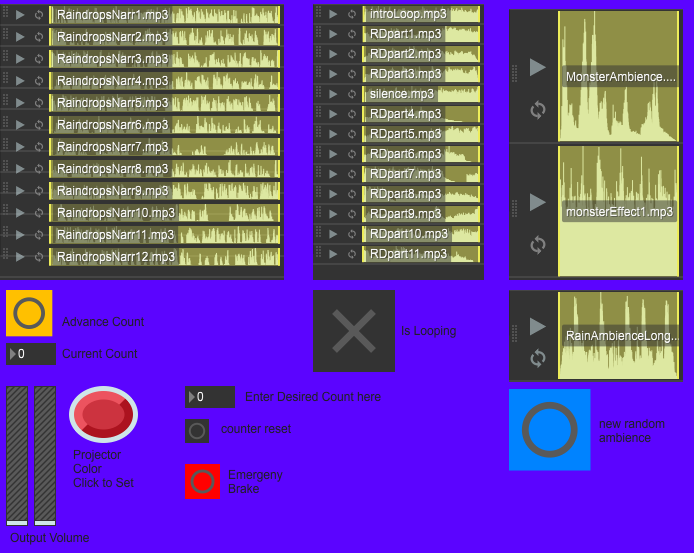
\includegraphics{diagrams/maxPatches/raindropspres.png}
    \caption{Raindrops on a Tin Roof Performer View}
    \label{fig:raindropsPres}
\end{figure}

\begin{figure}
    \centering
    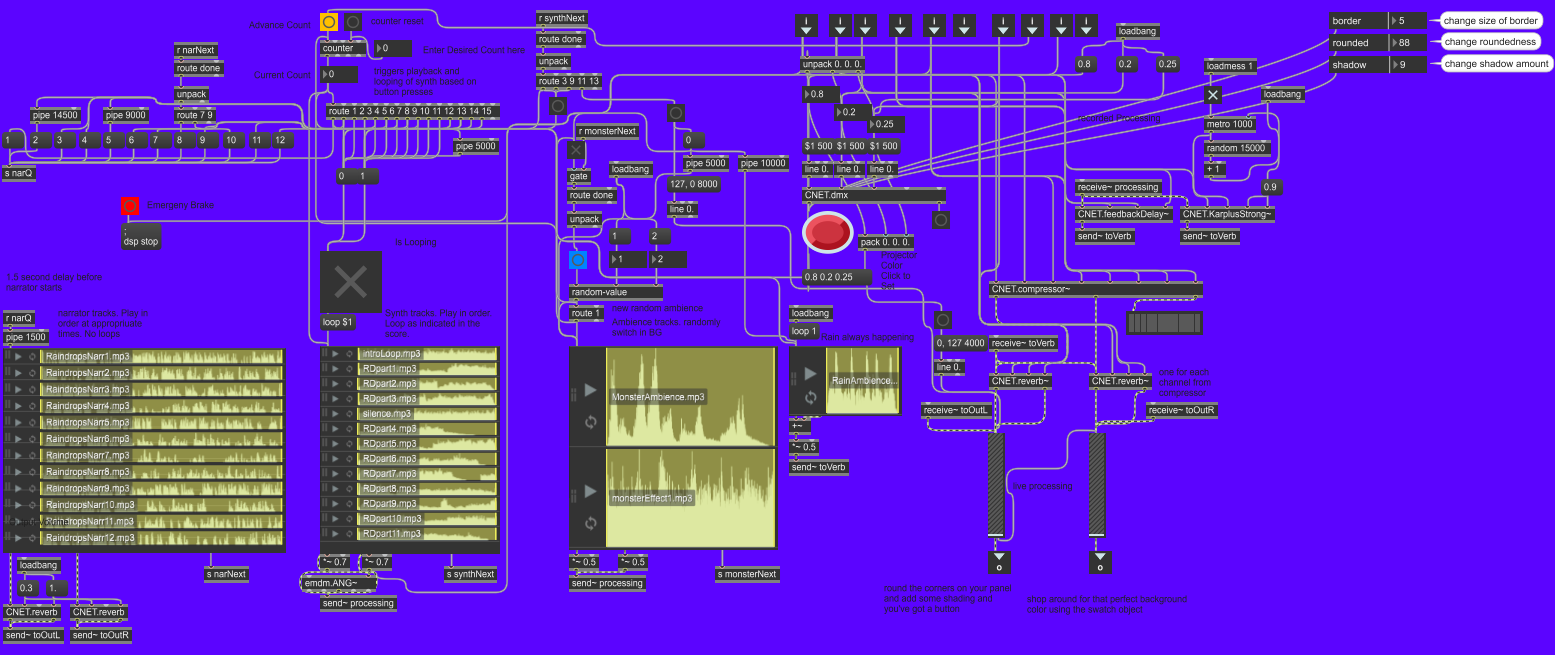
\includegraphics[scale=0.6]{diagrams/maxPatches/raindropsRaw.png}
    \caption{Raindrops on a Tin Roof Full View}
    \label{fig:raindropsRaw}
\end{figure}

\textit{Raindrops on a Tin Roof} was premiered by Adam Cope on 04/18/23 at the LSU Digital Media Center Theatre, but did not include the optional smoke machine.

\section{ImprovImpisaImptionImpprovisation in Reverb}
Similarly to \textit{Ethereal Presence}, \textit{ImprovImpisaImptionImpprovisation in Reverb} utilizes the gyroscope and accelerometer to control the computer processing. However instead of using the sensor data to control audio synthesis, this composition's algorithm controls multiple reverb and delay effects applied to the incoming signal from an onstage microphone.

\begin{figure}
    \centering
    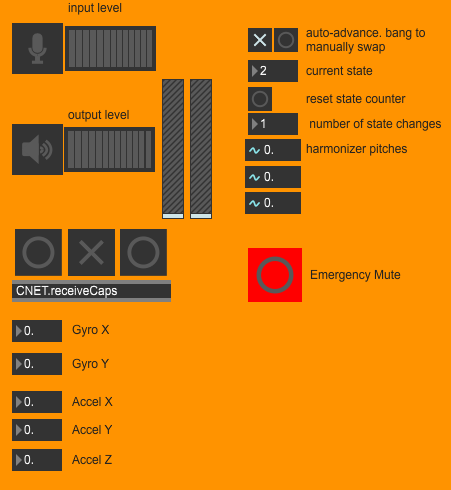
\includegraphics{diagrams/maxPatches/imporvPres.png}
    \caption{ImprovImpisaImptionImpprovisation in Reverb Performer View}
    \label{fig:ImprovPres}
\end{figure}

\begin{figure}
    \centering
    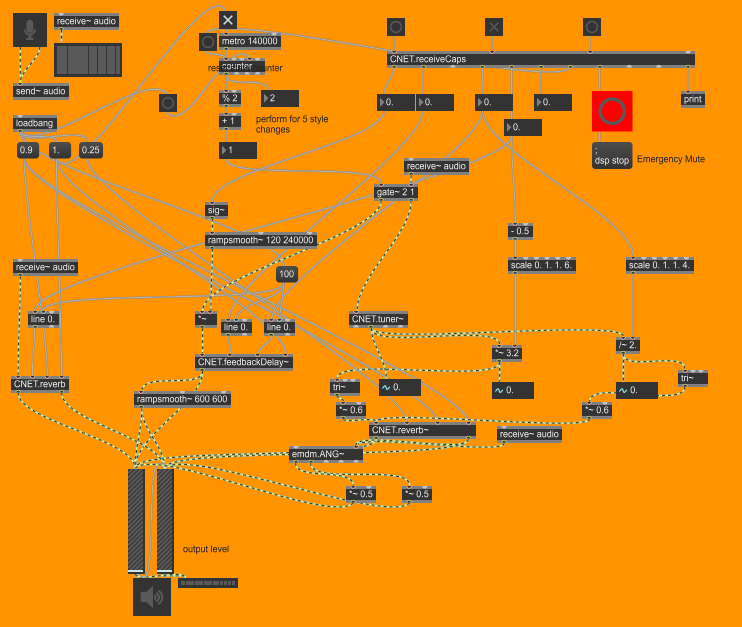
\includegraphics{diagrams/maxPatches/improvRaw.png}
    \caption{ImprovImpisaImptionImpprovisation in Reverb Full View}
    \label{fig:improvFull}
\end{figure}

The specific control mapping for this composition are as follows: 

\begin{itemize}
    \item GyroX: gates signal to CNET.feedbackDelay~
    \item GyroY: feedback delay time
    \item AccelX: feedback delay percentage and output gain, and low harmonizer pitch
    \item AccelY: high harmonizer pitch
\end{itemize}

Of the four compositions discussed in this chapter, \textit{ImprovImpisaImptionImpprovisation in Reverb} is the only one that does not have a dedicated score. This was done to focus on the potential use of the Cyberinet as an improvisation tool. By utilizing the movement data from the Cyberinet, the patch encourages the performer to explore the performance space. In terms of the physical movements required to trigger the effects, they are closest to those used in \textit{Ethereal Presence}. 

The max patch for this composition contains three main processes controlled by the Cyberinet. The first is a reverb effect that is constantly applied to the sound. The amount of reverb present changed based on the horizontal movement of the performer. Following that, the patch automatically swaps between two different states. The first is a feedback delay where the delay time is controlled again by horizontal movement. Specifically, the audio signal for this process is only fed into the delay line when the instrument has been shaken or is otherwise actively moving horizontally. The final state of the patch takes the signal and using CNET.tuner~ and CNET.pitchshift~, creates triangle waves that harmonize above and below the performer based on their Y-axis movement (upstage vs downstage). These states alter randomly for the duration of the performance, and are fed into additional, non-automated reverb effects as well as a patch which generates low-level background noise based on what is happening in the pitch-space of patch. If desired, the performer can utilize one of the buttons from the button expansion in order to both mute the soudn in an emergerncy, as well as manually swap between the mapping states.

This max patch utilizes a slightly different version of CNET.receive. This one is called CNET.receiveCaps. It is completely identical to CNET.receive in every way except that the labels used to route the sensor data all begin with capital letters. Because of the similarity with CNET.receive, this object is not discusses separately. It exists because the Cyberinet hardware used in the premiere of this work utilized an older version of the Arduino code that used capital letters instead of the camel-case that is conventional to modern coding. All versions of the Cyberinet following 1.2 use the preferred camel-case.

While not complex, this work emphasizes Van Nort's idea of a second-order level of gesture mapping\cite{vanNortMapping2007}. By being able to automatically or manually swap between the mapping states, the performer is able to further control and develop the relationship between sound and action. In a performance, the max patch will always default to the first state: the feedback delay. By having to move the instrument horizontally to activate the effect, the intention is that the listener will see the clear relationship between the two actions. Then, while not as drastic of an effect, the horizontal movement is utilized in the harmonization effect. The main control for the harmonizer is leaning back. Combined with a reverb effect that is always being affected by horizontal movement to act as an acoustic and gestural glue, the performer is able to create a clear relationship between the sounds and develop subtle variations between that relationship in a performance setting. I look forward to seeing future expansion on the idea of Second-Order gesture control with the Cyberinet in future compositions.

\textit{ImprovImpisaImptionImpprovisation in Reverb} was premiered on 05/01/2023 my Matthew A. Bardin in the LSU School of Music Recital Hall.

\section{Performer Opinions}
As previously stated, being a new augmented instrument, the aforementioned four works are the only compositions for the Cyberinet at the time of writing. To better inform future revisions and compositions, the two performers who premiered the above works were asked a series of questions following their usage of the Cyberinet. These questions were:

\begin{itemize}
    \item Question 1: How easy or difficult was it to implement the Cyberinet into your normal performance routine?
    \item Question 2: What was your favorite and least favorite part about working with the Cyberinet? 
    \item Question 3: How confident do you feel in being able to remove or add the Cyberinet to your clarinet in a performance setting?
    \item Question 4: How confident do you feel in being able to work with the Cyberinet's software capabilities to create unique sounds?
    \item Question 5: What thing or things did you dislike, or would change, about the Cyberinet?
\end{itemize}

In order to protect the identity of the performers, they are referred to by number. Performer 1's responses are shown below: % Adam

\begin{itemize}
    \item A1:
    \item A2:
    \item A3:
    \item A4:
    \item A5:
\end{itemize}

Following the initial performance, a studio recording of the works was made with Performer 1 and the questions were asked again. These are the responses to the same prompts following several weeks of additional practice and software adjustments set to improve the effect application in the premiere performance. 

\begin{itemize}
    \item A1:
    \item A2:
    \item A3:
    \item A4:
    \item A5:
\end{itemize}

The below responses belong to performer 2. % Me

\begin{itemize}
    \item A1: It was simple enough to implement, however there was a bit of a learning curve needed to reliably connect the device to the computer. Once I had the steps memorized it was reliable and simple to use.
    \item A2: My least favorite part was having to install all of the various drivers the first time. My favorite part was exploring with the gyroscope sensor and a reverb effect. the result was fun and intuitive.
    \item A3: I've already mentioned the issues in setting up the Cyberinet at the beginning, but being able to simply turn off the power and utilize the instrument completely acoustically as needed. This is easier than removing the unit.
    \item A4: I am already familiar with the Max environment so I feel that I could easily set up a lot of scenarios with the Cyberinet without much difficulties, but more reference material would be helpful. 
    \item A5: Other than the things I've already mentioned, I suppose I'd say relocating the port on the Button Expansion to a better location and potentially reducing the size of the main unit a little. It isn't too large, but a think a little smaller would be easier to work with.
\end{itemize}


%% The command ``\appendix'' switches into appendix-mode, meaning that subsequent ``\chapter'' commands will instead produce appendices.
\appendix

\chapter{Cyberinet Hardware Resources}
This appendix contains images for all of the 3D models and PCBs used within the Cyberinet. It also contains close-up images of each of the individual OEM sensors.

\section{3D models}
Below are all of the 3D models utilized to 3d print the case and accessories of the Cyberinet

\subsection{Main Body}

\begin{figure}
    \centering
    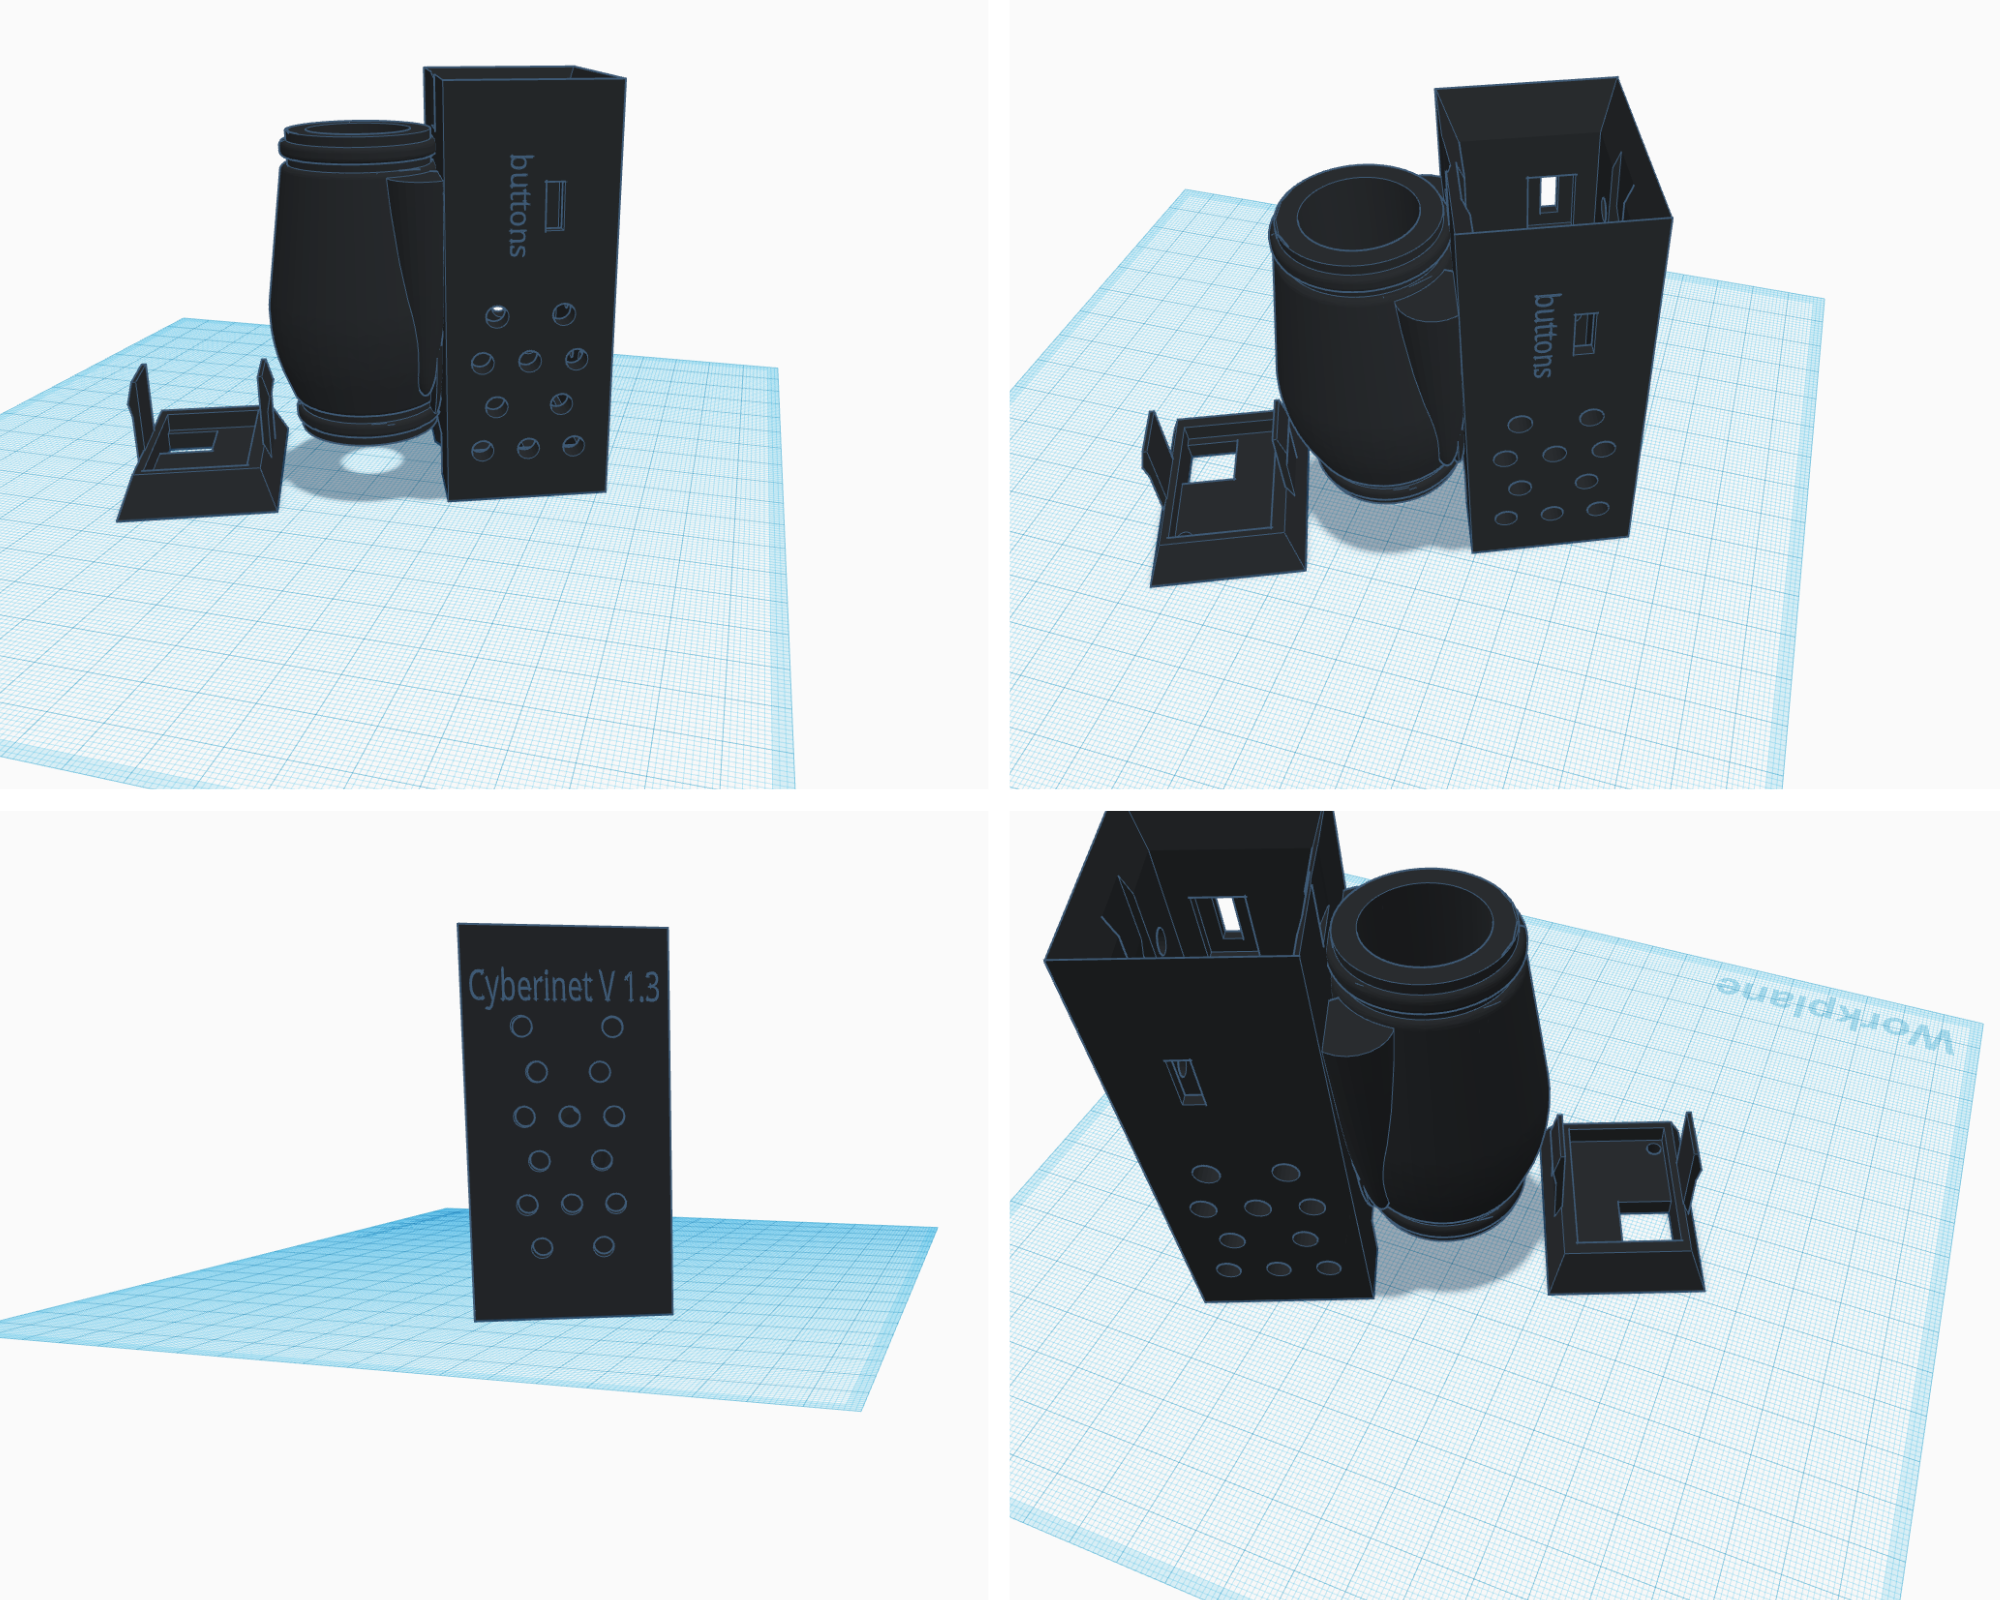
\includegraphics[scale=0.4]{diagrams/3D Models/Cyberinet main case 3d.png}
    \caption{Main Unit of the Cyberinet from various angles}
    \label{fig:main3D}
\end{figure}



\subsection{Button Board Thumbrest Mount}

\begin{figure}
    \centering
    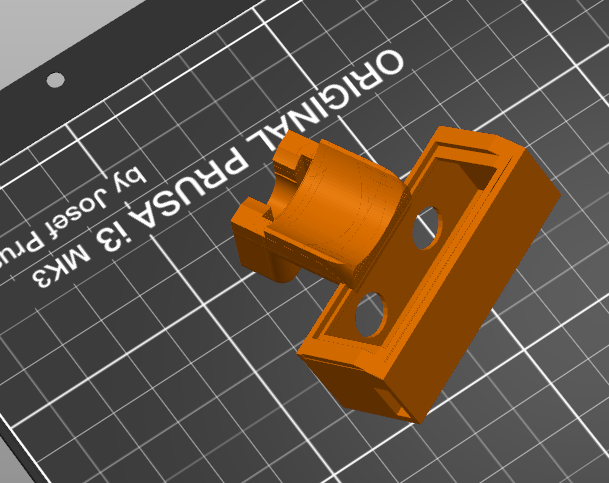
\includegraphics[scale=0.8]{diagrams/3D Models/thumbrestPic.png}
    \caption{Button Board Thumbrest Mount in 3D printing software}
    \label{fig:thumbrest}
\end{figure}



\section{PCB Diagrams}
Below are the PCB diagrams for the Cyberinet. Main unit and Button Expansion


\begin{center}
\begin{figure}
    \centering
    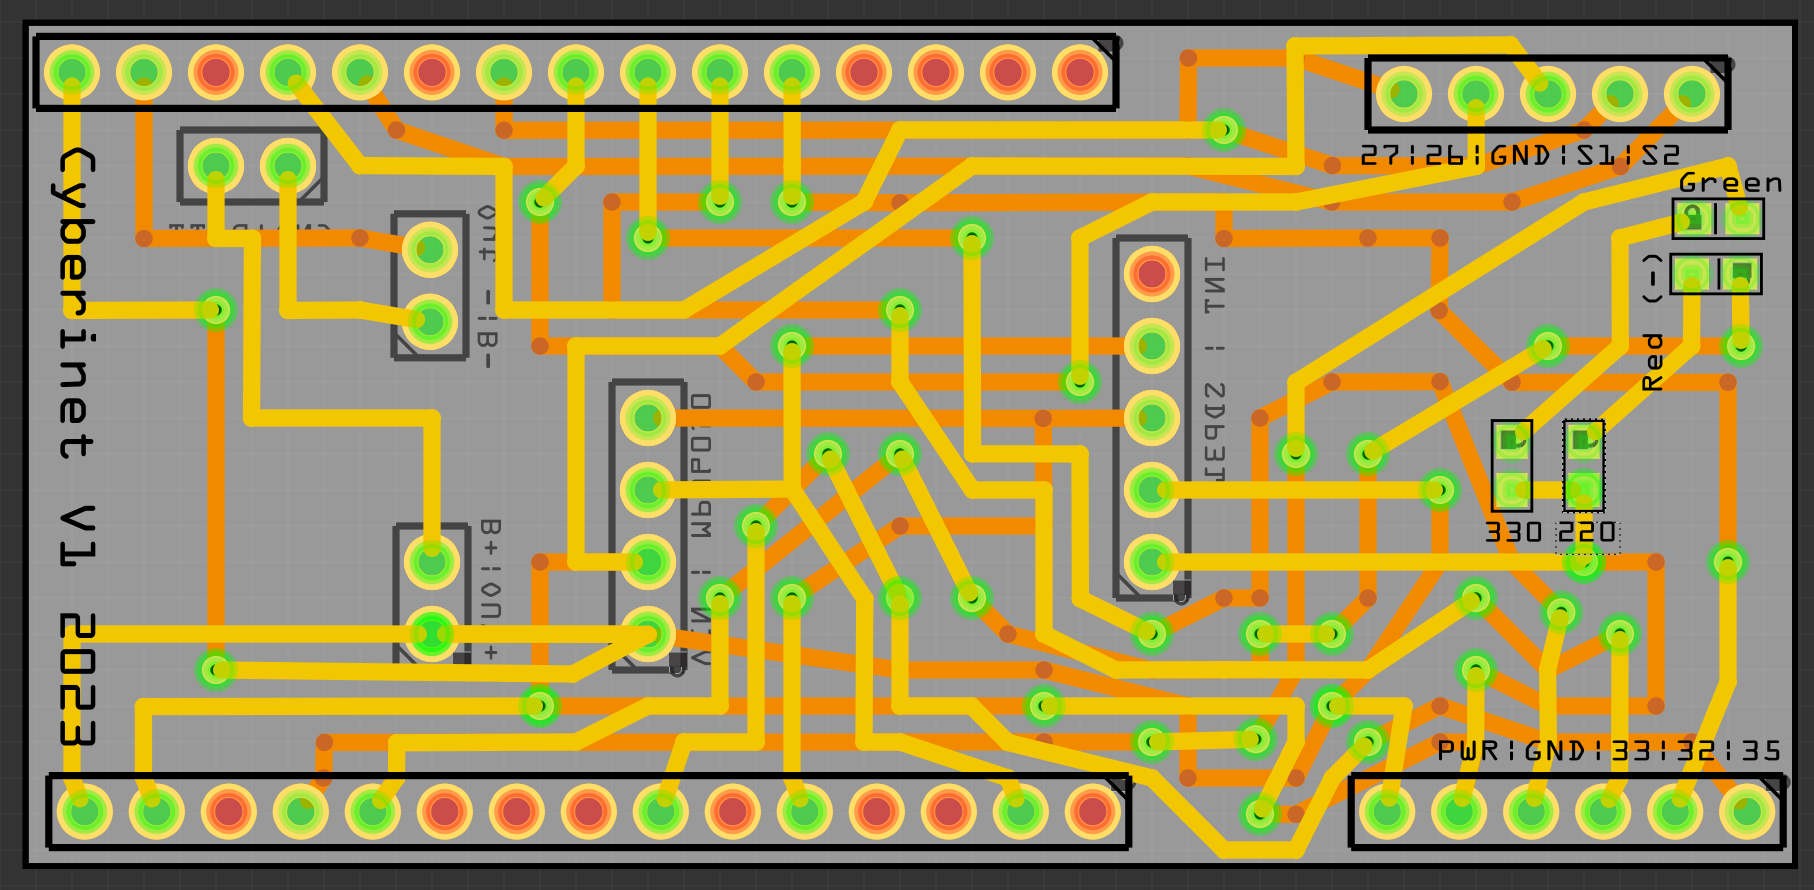
\includegraphics[scale=0.3]{diagrams/PCBs/mainBoard.png}
    \caption{Cyberinet Main Unit PCB}
    \label{fig:mainPCB}
\end{figure}
\end{center}



% \section{OEM Components Detailed Photos}

% \begin{center}
%     \begin{figure}
%         \centering
%         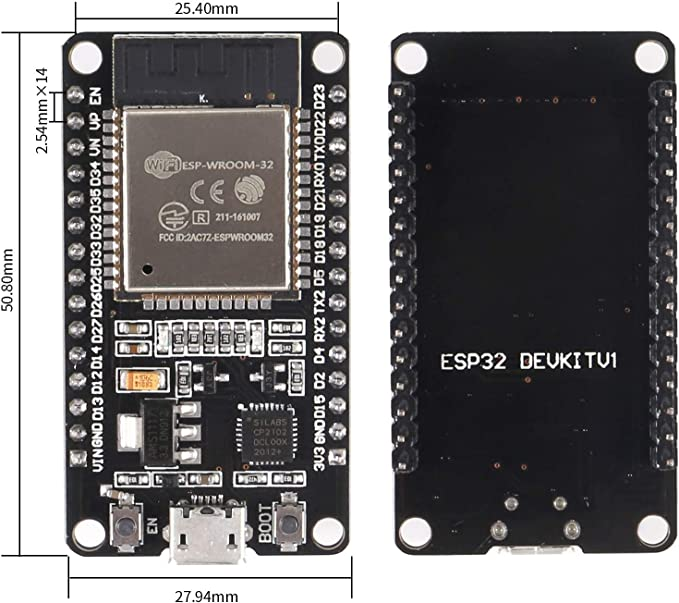
\includegraphics[scale=0.3]{diagrams/oem/esp-32.jpg}
%         \caption{ESP-32 DEVKIT V1 Micro-controller}
%         \label{fig:ESP-32.2}
%     \end{figure}
% \end{center}

% \begin{center}
%     \begin{figure}
%         \centering
%         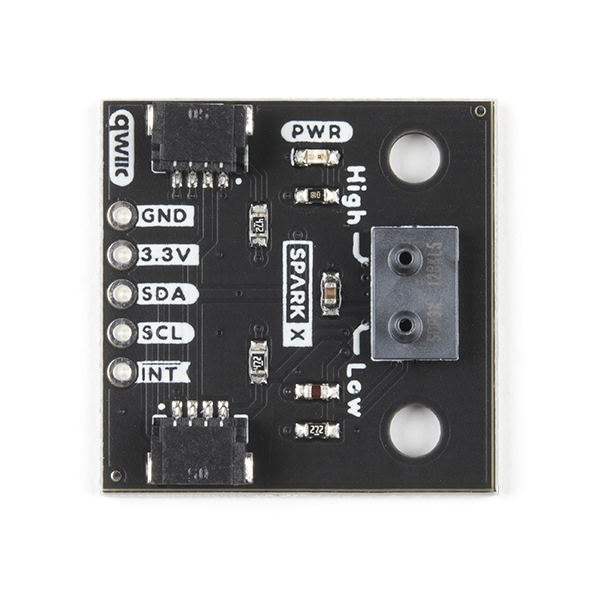
\includegraphics{diagrams/oem/spd31.jpg}
%         \caption{Sparkfun SDP-31 Differential Airflow Pressure Qwiic Connect Breakout Board}
%         \label{fig:sdp-3.2}
%     \end{figure}
% \end{center}


% \begin{center}
%     \begin{figure}
%         \centering
%         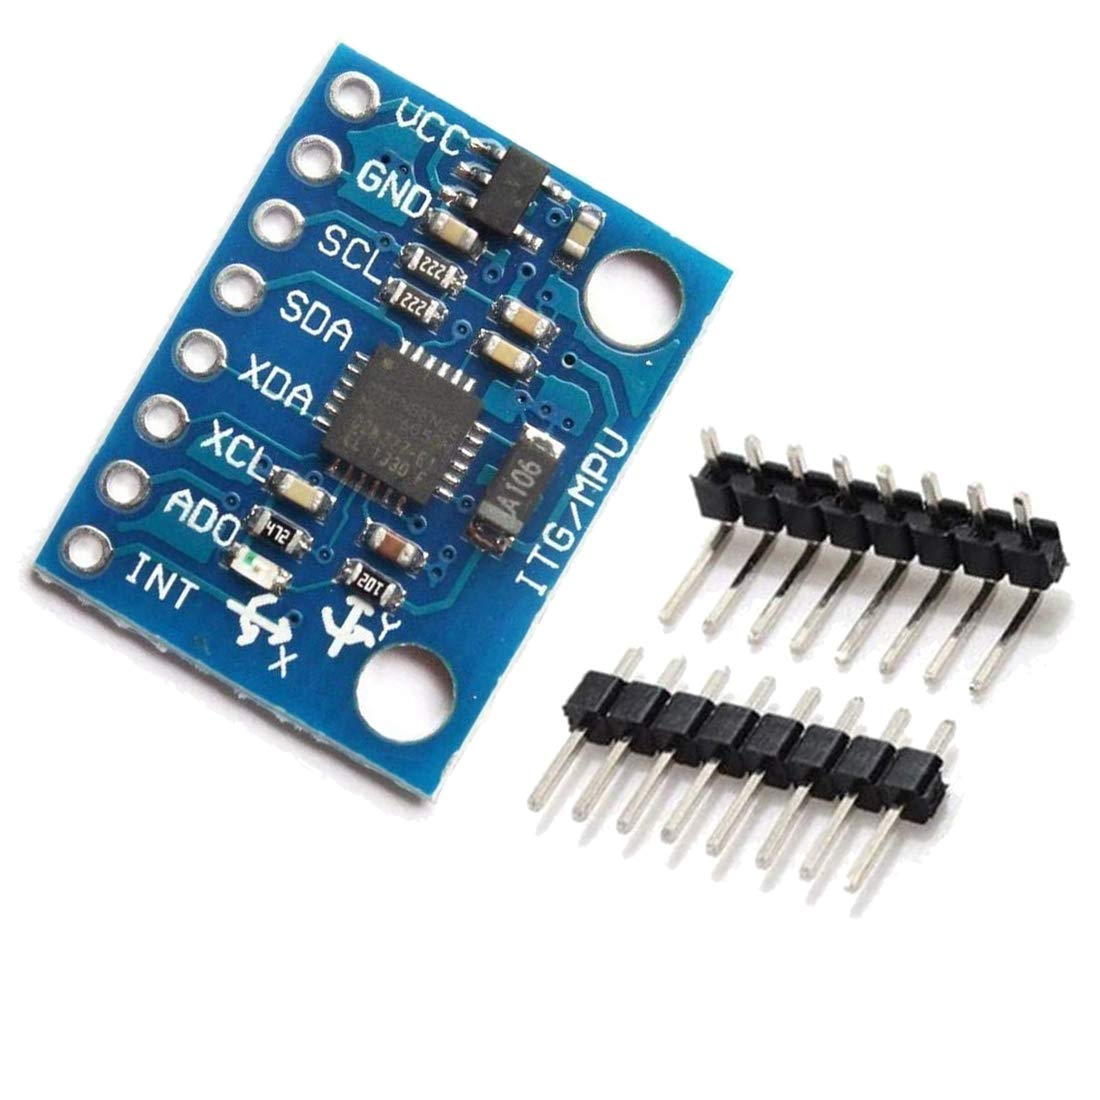
\includegraphics[scale=0.2]{diagrams/oem/6050.jpg}
%         \caption{MPU-6050 Gyroscope and Accelerometer}
%         \label{fig:6050.2}
%     \end{figure}
% \end{center}

% \begin{center}
%     \begin{figure}
%         \centering
%         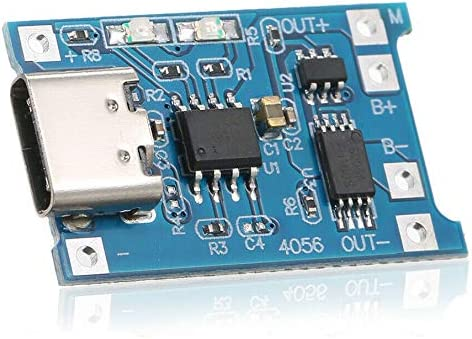
\includegraphics[scale=0.3]{diagrams/oem/4056.jpg}
%         \caption{TP-4056 Type C LiPo Battery Charger}
%         \label{fig4055.2}
%     \end{figure}
% \end{center}




\chapter{Cyberinet Software Components}
This appendix contains all of the Arduino code flashed to the Cyberinet. (Version 1.3), as well as screenshots of the various max patches and objects included in the software bundle.

\section{Arduino .ino Code}

Below is the .ino code that is running on the ESP-32 micro-controller. This code was developed using the Arduino IDE and coding language.

\begin{verbatim}

/*
    Micro Controller Code for the Cyberinet Version 1.3
   Code designed for the ESP-32 WROOM DEVKIT V1 in the Arduino IDE.
   All Serial Communications are over Bluetooth.
   Code may be used or reworked with Attribution.
   Altering code present on Cyberinet unit is not recommended.
   Code and Other Matierials for the Cyberinet can 
   be found at https://github.com/mbardin/Cyberinet
   Code and Other Marerials made 
   by Matthew A. Bardin [2023] (https://matthewbardin.com)
*/

//libraries to include
#include <SparkFun_SDP3x_Arduino_Library.h>
#include<Wire.h>
#include <BluetoothSerial.h>
#include <MPU6050.h>


// create instances of the libraries above
BluetoothSerial SerialBT;
MPU6050 mpu;
// constant sensing is on I2C address 0x21
SDP3X airFlow;


// Global Variables
// dedicated pins
const int pwrLED = 2; // green 330 Ohm
const int msgLED = 4; // red 220 Ohm
const int button1 = 12;
const int button2 = 14;
const int b1LED = 26;
const int b2LED = 27;
const int expPin1 = 33;
const int expPin2 = 32;
const int expPin3 = 35;
const int expPin4 = 18;

// MPU 6050 values
const int MPU_ADDR = 0x68; // I2C address of the MPU-6050
int16_t AcX, AcY, AcZ, GyX, GyY, GyZ; // values for 6050
// store mapped values for transmitting
float rotX, rotY, rotZ, gForceX, gForceY, gForceZ; 

// stores current button state
int button1State = 1;
int button2State = 1;

// store SDP31 values for transmitting
//float diffPressure = 0.0;
//float temperature = 0.0;

// store exp values for transmitting
int exp1State = 0;
int exp2State = 0;
int exp3State = 0;
int exp4State = 0;

void setup() {
  // Pin mode assignment
  pinMode(pwrLED, OUTPUT);
  pinMode(msgLED, OUTPUT);
  // use ESP32's built in pullup resistors
  pinMode(button1, INPUT_PULLUP); 
  pinMode(button2, INPUT_PULLUP);

  Serial.begin(115200);
  / Device name. no spaces or punctuation
  SerialBT.begin("CyberinetV13"); 
  delay(1000); // pause before checking
  // various startup and checks
  gyroStartup();
  airflowStartup();
  startLights();
}



void loop() { // check the sensors and transmit each loop.
  get6050();
  getButtons();
  getExp();
  getAir(); // put 6050 and sdp31 on ends of sensor checks
}


void get6050() {

  ////////////Collect Data
  Wire.beginTransmission(MPU_ADDR);
  Wire.write(0x3B);  // wake up device
  Wire.endTransmission(true);

  Wire.requestFrom(MPU_ADDR, 6); 
  while (Wire.available() < 6);
  AcX = Wire.read() << 8 | Wire.read(); 
  AcY = Wire.read() << 8 | Wire.read(); 
  AcZ = Wire.read() << 8 | Wire.read(); 

  Wire.beginTransmission(MPU_ADDR); //I2C address of the MPU
  Wire.write(0x43); 
  Wire.endTransmission();
  Wire.requestFrom(MPU_ADDR, 6); /)
  while (Wire.available() < 6);
  GyX = Wire.read() << 8 | Wire.read();
  GyY = Wire.read() << 8 | Wire.read();
  GyZ = Wire.read() << 8 | Wire.read();


  ////////////Format Data
  rotX = GyX *  0.007633587786; 
  rotY = GyY *  0.007633587786;
  rotZ = GyZ *  0.007633587786;

  gForceX = AcX * 0.00006103515;
  gForceY = AcY * 0.00006103515;
  gForceZ = AcZ * 0.00006103515;


  ////////////Transmit Data
  digitalWrite(msgLED, HIGH); 
  SerialBT.print("gyroX "); // label
  SerialBT.println(rotX); // value

  SerialBT.print("gyroY "); // label
  SerialBT.println(rotY); // value

  SerialBT.print("gyroZ "); // etc.
  SerialBT.println(rotZ);

  SerialBT.print("accelX ");
  SerialBT.println(gForceX);

  SerialBT.print("accelY ");
  SerialBT.println(gForceY);

  SerialBT.print("accelZ ");
  SerialBT.println(gForceZ);
  digitalWrite(msgLED, LOW);
}

void getButtons() {
  ////////////Collect Data
  button1State = digitalRead(button1);
  button2State = digitalRead(button2);

  ////////////Transmit Data 
  digitalWrite(msgLED, HIGH); // turn LED on when tranmitting data
  SerialBT.print("b1 "); // label
  SerialBT.println(button1State); // value
  // on-board led state matches button state
  digitalWrite(b1LED, button1State); 
  // repeat for other button
  SerialBT.print("b2 ");
  SerialBT.println(button2State);
  digitalWrite(b1LED, button2State);
  digitalWrite(msgLED, LOW); // turn off led when done transmitting
}


void getExp() {
  // Look at each return pin
  exp1State = digitalRead(expPin1);
  exp2State = digitalRead(expPin2);
  exp3State = digitalRead(expPin3);
  exp4State = digitalRead(expPin4);

  // transmitData
  digitalWrite(msgLED, HIGH);
  SerialBT.print("exp1 ");
  SerialBT.println(exp1State);
  SerialBT.print("exp2 ");
  SerialBT.println(exp2State);
  SerialBT.print("exp3 ");
  SerialBT.println(exp3State);
  SerialBT.print("exp4 ");
  SerialBT.println(exp4State);
  digitalWrite(msgLED, LOW);
}

void getAir() {
  ////////////Collect Data
  // Storage for the differential pressure
  float diffPressure; 
  // Storage for the temperature
  float temperature; 
  airFlow.readMeasurement(&diffPressure, &temperature);

  ////////////Transmit Data
  digitalWrite(msgLED, HIGH); // turn on LED when tranmitting
  SerialBT.print(F("airP ")); // lebel
  SerialBT.println(diffPressure, 2); // value

  SerialBT.print(F("temp "));
  SerialBT.println(temperature, 2);
  digitalWrite(msgLED, LOW); // turn of LED when done transmitting
}


// startup functions
void gyroStartup() {
  Wire.begin(21, 22, 100000); // sda, scl, clock speed
  Wire.beginTransmission(MPU_ADDR);
  Wire.write(0x6B);  // PWR_MGMT_1 register
  Wire.write(0);     // (wakes up the MPU−6050)
  Wire.endTransmission(true);
  SerialBT.println("MPU-6050 Setup Complete");
}

void airflowStartup() {
  // Initialize sensor. Stops if connection cannot be made
  airFlow.stopContinuousMeasurement();

  if (airFlow.begin() == false)
  {
    SerialBT.println(F("SDP31 not detected.));
    while (1);
  }
  // set to continuous measurement mode
  airFlow.startContinuousMeasurement(true, true); 
  SerialBT.println("SDP31 Setup Complete");
}

void startLights() { // flashes startup LED in apecific pattern
  digitalWrite(pwrLED, HIGH);
  digitalWrite(msgLED, HIGH);
  delay(500);
  digitalWrite(msgLED, LOW);
  delay(500);
  digitalWrite(msgLED, HIGH);
  delay(500);
  digitalWrite(msgLED, LOW);
  delay(1000);
  digitalWrite(msgLED, HIGH);
  delay(1000);
  digitalWrite(msgLED, LOW);
}

\end{verbatim}

\section{Max Objects}
This section discusses each of the CNET objects that were created with the intention of interfacing with the Cyberinet. With the exception of CNET.receive, these are smaller objects designed to easily implement the Cyberinet into some of the common audio effects the user is likely already implementing in Max. Because of how CNET.receive works, these objects are not required to utilize the Cyberinet, but are recommended for people learning how to work with Max or the Cyberinet for the first time.

Each object listed here also has a help patch which walks the user through setup and adjusting the values for that object. The help patches do not need the Cyberinet to be connected to work, and contain 3 different presets to show a variety of sound options. All inlets for these object utilize a 0-1 floating point number for parameter control. Default values for these inlets are all given in the help patches.

\subsection{Functional Objects}
These objects serve to increase the functionality of the Cyberinet and do not alter sound sources or control other objects.

\subsubsection{CNET.receive}
This is the only required object in the CNET collection. This object is responsible for setting up communications with the Cyberinet, parsing the data, and outputting it to the various outlets. Each sensor on the Cyberinet has a dedicated outlet, so connecting to each outlet will always relay the same sensor. The outlet order is given below.

\begin{enumerate}
    \item gyroX
    \item gyroY
    \item gyroZ
    \item accelX
    \item accelY
    \item accelZ
    \item b1
    \item b2
    \item airP
    \item temp
    \item exp
    \item errorMsg
\end{enumerate}

The final outlet will output an error indicating that CNET.receive received a message it did not recognize, as well as the error causing message.

To establish communications, bangs and toggles are utilized in order to simplify the interface. The user inputs a bang to the first inlet to start the script and list the available ports. When paired to the computer via Bluetooth, the Cyberinet will appear on the list of available ports. The user can then set the port by filling in the message box connected to inlet 2, and receive communications with a bang to the third inlet. Inlet 4 will stop all communications. The process will have to be repeated to initialize them again, and a bang to inlet 5 will install necessary node package manager dependencies and drivers the first time a computer is utilizing the Cyberinet.

The Node script and functionality comes from a package created by the LSU Experimental Music \& Digital Media department, and the JavaScript code for this is shown below in its entirety.

\begin{verbatim}
// EMDM Serial communications in Max
const path = require('path');
const Max = require('max-api');

const { SerialPort, ReadlineParser } = require('serialport')
const baud = 115200;
let devicePort = '/dev/tty-CyberinetV13'

// Create a port
let port;
let availablePorts;
let parser = new ReadlineParser();


Max.post(`Loaded the ${path.basename(__filename)} script`);

Max.addHandler("bang", () => {
	Max.post("Who you think you bangin'?");
});

Max.addHandler("echo", (msg) => {
	Max.outlet(msg);
});

Max.addHandler("portlist", () => {
  SerialPort.list().then((ports)=>{
    Max.post("Ports: ", ports);
    console.log(ports);
    availablePorts = ports;
  });
});

Max.addHandler('setPort', (port) => {
  devicePort = port;
})

Max.addHandler('open', () => {
  port = new SerialPort({
    path: devicePort,
    baudRate: baud,
  }, function (err) {
    if (err) {
      return console.log('Error: ', err.message)
    }
  })
})

Max.addHandler('enable', () => {
  Max.post('Serial Receive Enabled');

  port.pipe(parser)
  parser.on('data', (cyberData)=>{
    let cyber = cyberData.split(" ");
    let sensor = cyber[0];
    let value = parseFloat(cyber[1]);
    Max.outlet(sensor, value);
  })
})

Max.addHandler('send', (data) => {
  port.write(data, function(err) {
    if (err) {
      return console.log('Error on write: ', err.message)
    }
    console.log('message written')
  })
})
\end{verbatim}

In short, after setting up the port communications, this code will identify the label:value pair and output them separated by a space via the outlet in the Node object. From there, a Max route object separates the values to different outlets based on the labels shown above. Values are scaled to fit a range of 0-1 where appropriate.

\subsubsection{CNET.rangeSet}
Used for adjusting the value scaling within CNET.receive. This object is used to fine tune the ranges expected for a performer with their Cyberinet unit. Maximum and minimum sensor values can be determined by looking at the Max terminal when the raw outputs are being displayed. Ranges are set to a specific sensor utilizing the same labels as those used in CNET.receive. Setting the sensor label with a message or sending a bang to the first outlet will trigger a list to be output from this object.

Within CNET.receive, an additional route and a handful of unpack objects are used to properly apply the data. All values leaving CNET.receive are still mapped to a range of 0-1 after this new scaling occurs.

\begin{figure}
    \centering
    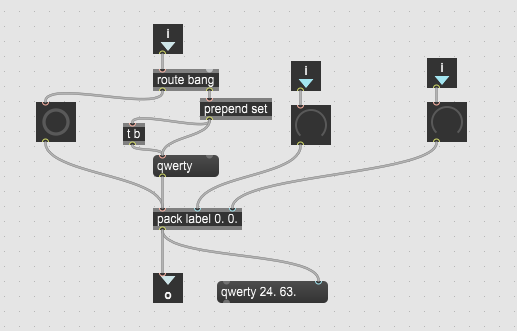
\includegraphics{diagrams/maxPatches/CNET.rangeSet.png}
    \caption{CNET.rangeSet.maxpat}
    \label{fig:CNET.rangeSet.maxpatch}
\end{figure}

\subsubsection{CNET.latency~}
Used to calculate the latency between the Cyberinet detecting a sensor value change on the hardware, and that change being reflected in the Max environment. To achieve this, a microphone is needed. 

To test the latency, first you must connect the Cyberinet using CNET.receive, and ensure that the Button expansion is connected. 

Using the patch, a sound file is recorded. One channel of the stereo file records the sound of a button clicking on the Cyberinet. This button press is used to generate a pulse of white noise on the second channel.

The recordings are then compared to determine the time between the real-world action and the software response which is represented in milliseconds for the user. Large objects located between the computer and the Cyberinet may negatively affect the latency.

\subsubsection{CNET.tuner~}

This object is a simple tuner based off of the retune~ object native to Max. It receives a signal from an external microphone and outputs both the closest MIDI pitch and frequency of the sound. These values are output as signals. In this version of the Cyberinet, it must be located in the Max software as the ESP-32's ADC's are not powerful enough to run a tuner along with everything else. It is recommended for both tuning purposes, as well as pitch identification purposes. 
% made weird things appear on first page when not uncommented???????????????
% \begin{figure}
%     \centering
%     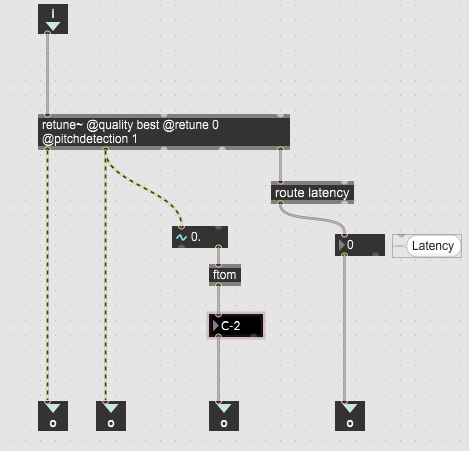
\includegraphics{diagrams/maxPatches/CNET.tuner~.png}
%     \caption{CNET.tuner~.maxpat}
%     \label{fig:CNET.tuner~.maxpat}
% \end{figure}
 

\subsubsection{CNET.click~}
This object is able to receive a BPM value and outputs both a bang in Max, but also sends an audio signal click. This signal can be used by connecting a [receive~ click] to the desired output. For the compositions discussed in this document, the click track was always connected to channel 3 of the audio interface.

\begin{figure}
    \centering
    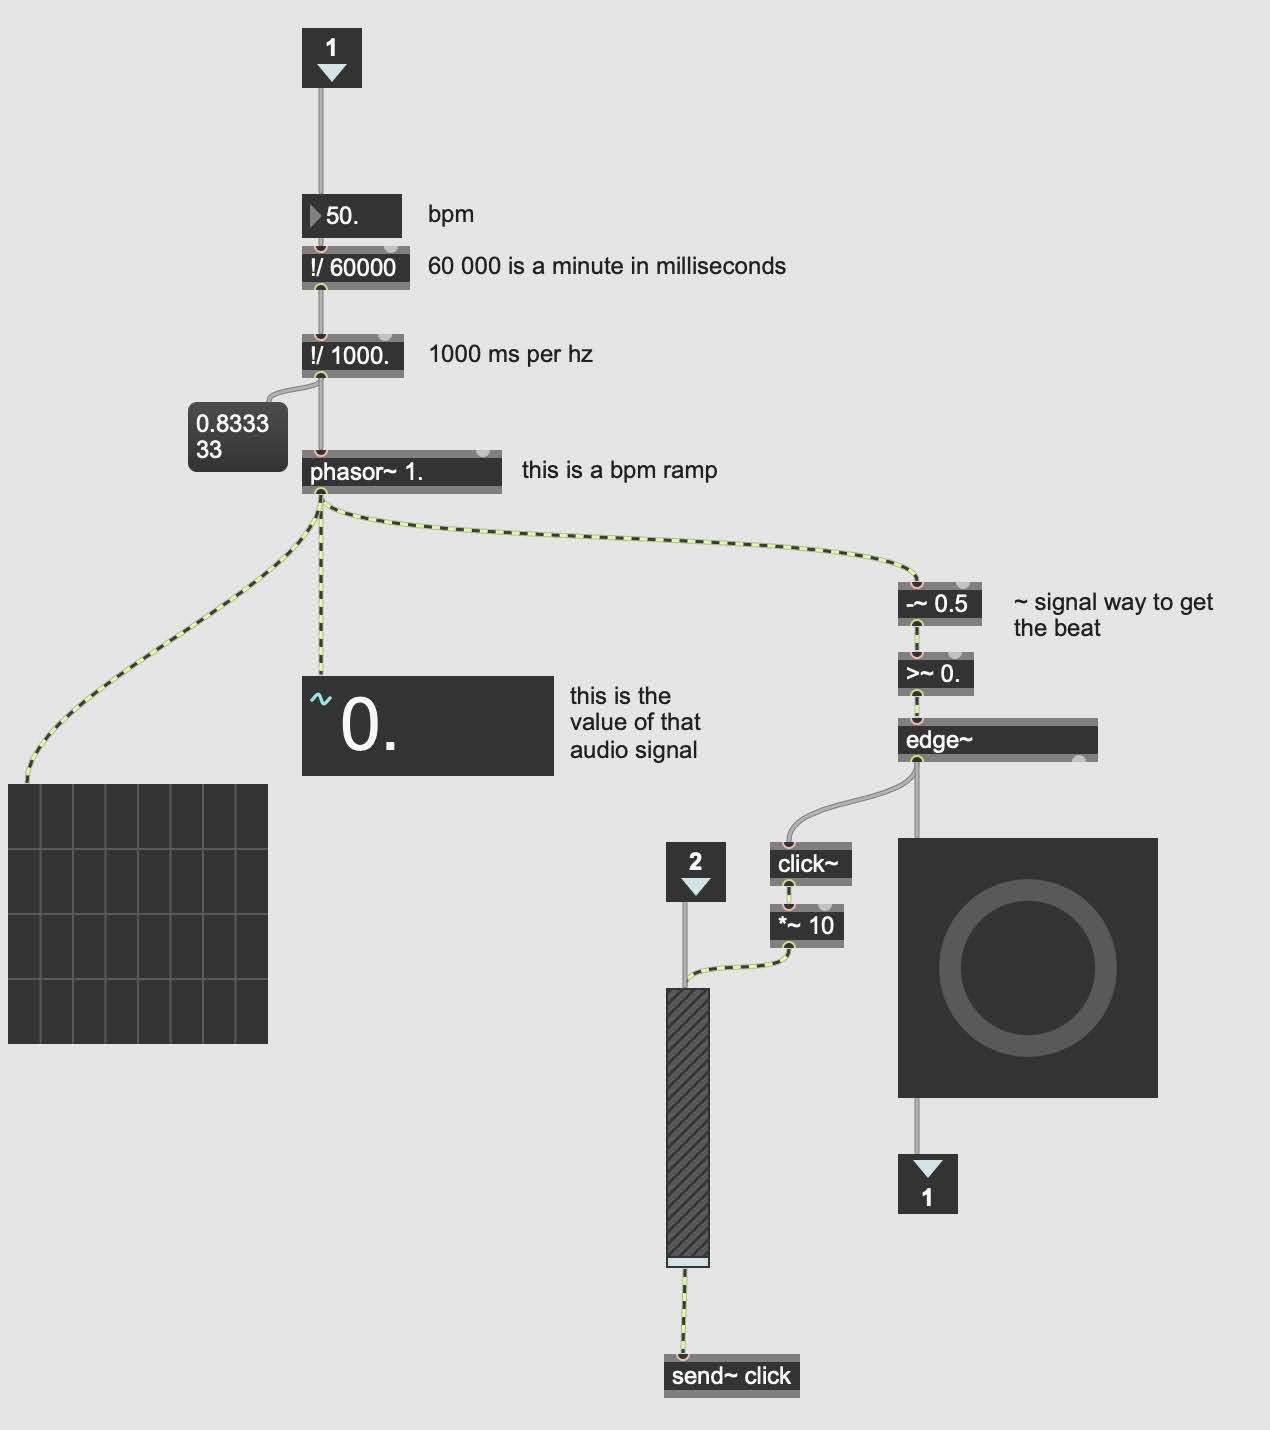
\includegraphics[scale=0.2]{diagrams/maxPatches/CNET.click~.jpg}
    \caption{CNET.click~ max patch}
    \label{fig:CNET.clickPAtch}
\end{figure}

\subsubsection{CNET.pan}
I was unsure about which section to place this object in. I chose its ultimate placement here as the object is not directly changing the sound, but rather it receives data to control the stereo panning of a signal.

\subsubsection{CNET.dmx}
This object functions to allow the Cyberinet to control DMX lighting with its various sensors. Note that this will not work with every DMX controller, and is specifically designed to interface with the Chauvet DMX-AN 2. After being setup with the desired environmental settings, CNET.dmx takes in three sensor readings to control the red, green, and blue levels of the connected lights.

\begin{figure}
    \centering
    \includegraphics[scale=0.85]{diagrams/maxPatches/CNET.dmx.png}
    \caption{CNET.dmx.maxpat}
    \label{fig:CNET.dmx.maxpat}
\end{figure}

\subsection{Audio Effects}
These audio effects are designed to receive information from the functional objects above and utilize the data to either process sound or control another object. Generally, these effects are relatively simple alterations of sounds similar to audio effects found in most DAW's.

\subsubsection{CNET.reverb~}
This is a stereo Schroder reverb internally similar to the popular JC reverb developed by John Chowning. Type more here about the effect. Include how it works, the parameters that can be controlled, and anything unique about it. 

\begin{figure}
    \centering
    \includegraphics{diagrams/maxPatches/CNET.reverb~.png}
    \caption{CNET.reverb~.maxpat}
    \label{fig:my_label}
\end{figure}

\subsubsection{CNET.monoReverb~}
This patch is identical to CNET.reverb~, except that it outputs a mono signal instead of stereo.

\subsubsection{CNET.compressor~}
CNET.compressor is a fairly standard compressor that is able to receive data from the Cyberinet in order to control the threshold, ratio, attack, release, and gain staging before and after the effect. By connecting a meter~ object to the last outlet, a faux VU meter can be created to show the gain reduction happening in the compressor.

\begin{figure}
    \centering
    \includegraphics{diagrams/maxPatches/CNET.compressor~.png}
    \caption{CNET.compressor~.maxpat}
    \label{fig:compmax}
\end{figure}

One unique feature of this compressor is that it takes in a mono signal and outputs a stereo signal.
% made weird things appear on first page when not uncommented???????????????
% \begin{figure}
%     \centering
%     \includegraphics{diagrams/maxPatches/compInner.png}
%     \caption{inner workings of CNET.compressor~}
%     \label{fig:compressor~Inner}
% \end{figure}

\subsubsection{Various Delays}
A total of four various delays have been created for a variety of different audio effects. these include:

\begin{itemize}
    \item CNET.delay~: a simple delay of an audio signal.
    \item CNET.feedbackDelay~: a delay with an adjustable feedback percentage
    \item CNET.multDel~: a delay with four individually controllable delay lines
    \item CNET.vibDelay~: a delay line that also creates a vibrato effect on the delayed signal.
\end{itemize}

\begin{figure}
    \centering
    \includegraphics{diagrams/maxPatches/CNET.delay~.png}
    \caption{CNET.delay~.maxpat}
    \label{fig:delMaxpat}
\end{figure}

\begin{figure}
    \centering
    \includegraphics{diagrams/maxPatches/CNET.feedbackDelay~.png}
    \caption{CNET.feedbackDelay~.maxpat}
    \label{fig:fbDelMaxpat}
\end{figure}

\begin{figure}
    \centering
    \includegraphics[scale=0.7]{diagrams/maxPatches/CNET.multDel~.png}
    \caption{CNET.multDel~.maxpat}
    \label{fig:multDel}
\end{figure}

\begin{figure}
    \centering
    \includegraphics[scale=0.8]{diagrams/maxPatches/CNET.vibDelay~.png}
    \caption{CNET.vibDelay~.maxpat}
    \label{fig:vibDel}
\end{figure}

\subsubsection{CNET.karplusStrong~}
This patch works by taking the incoming audio signal as a sample. When triggered, the algorithm generates a plucked-string sound utilizing this source signal. The end result is a pluck sound that will match up with the incoming sounds, and can be triggered on-demand. The filter coefficient, approximate pitch of the resulting 'pluck', and the effect's output volume are all controlled with the Cyberinet.

\begin{figure}
    \centering
    \includegraphics{diagrams/maxPatches/CNET.kStrong.png}
    \caption{CNET.karplusStrong~.maxpat}
    \label{fig:kstrong}
\end{figure}

\subsubsection{CNET.pitchShift~}

\begin{figure}
    \centering
    \includegraphics{diagrams/maxPatches/CNET.pitchShift~.png}
    \caption{CNET.pitchShift~.maxpat}
    \label{fig:pitchshift}
\end{figure}


% make sure most up-to-date pdf is shown here
\chapter{Puzzle of a Park Full Score}

\includepdf[pages=1-13]{Scores/PPFull.pdf}

\chapter{Ethereal Presence Full Score}

\includepdf[pages=1-9]{Scores/EP.pdf}

\chapter{Raindrops on a Tin Roof}

\section{Full Score}
Pages are scaled down from the Tabloid (11in by 17in) size of the original score to match the rest of this document. 

\includepdf[pages=1-19]{Scores/raindrops.pdf} 
%  list page range and file location

\section{Short Story Text}

\includepdf[pages=1-4]{Scores/Raindrops Text.pdf}



\chapter{Permissions}

% The ``permissions'' area reproduces requests and permissions for previously published material or material belonging to others. If included, then it should be the last appendix.
I'm assuming this is where I will put the various permissions from the images?


\backmatter
%%%%%%%%%%%%%%%%%%%%%%%%%%%%%%%%%%%%%%%%%%%%%%%%%%%%%%%%%%%%%%
%%%%%%%%%%%%%%%%%%%%%%%%%%%%%%%%%%%%%%%%%%%%%%%%%%%%%%%%%%%%%%
%%%%%%%%%%%%%%%%%%%%%%%%%%%%%%%%%%%%%%%%%%%%%%%%%%%%%%%%%%%%%%
%%%%%%%%%%%%%%%%%%%%%%%%%%%%%%%%%%%%%%%%%%%%%%%%%%%%%%%%%%%%%%
%%%%%%%%%%%%%%%%%%%%%%%%%%%%%%%%%%%%%%%%%%%%%%%%%%%%%%%%%%%%%%
% Jesse if you read this before our mext meeting, chould I use the NIME formatting as a template?
% I've read so many different kinds of stuff for this the formatting hasn't been consistent and I'm not sure which one to use.
%%%%%%%%%%%%%%%%%%%%%%%%%%%%%%%%%%%%%%%%%%%%%%%%%%%%%%%%%%%%%%%
%%%%%%%%%%%%%%%%%%%%%%%%%%%%%%%%%%%%%%%%%%%%%%%%%%%%%%%%%%%%%%%
%%%%%%%%%%%%%%%%%%%%%%%%%%%%%%%%%%%%%%%%%%%%%%%%%%%%%%%%%%%%%%%
%%%%%%%%%%%%%%%%%%%%%%%%%%%%%%%%%%%%%%%%%%%%%%%%%%%%%%%%%%%%%%%
%%%%%%%%%%%%%%%%%%%%%%%%%%%%%%%%%%%%%%%%%%%%%%%%%%%%%%%%%%%%%%%


\begin{thebibliography}{99} % double check the formatting for the EMDM citations. Include template in comments here

% \bibitem{label}

\bibitem{puzzleScore} Bardin, Matthew. \emph{Puzzle of a Park} Performance Score, MaBMusic, 2023.

\bibitem{EPScore} Bardin, Matthew. \emph{Ethereal Presence} Performance Score, MaBMusic, 2023.

\bibitem{Raindrops Score} Bardin, Matthew. \emph{Raindrops on a Tin Roof} Performance Score, MaBMusic, 2023.

\bibitem{Raindrops Story} Bardin, Matthew. \emph{Raindrops on a Tin Roof} Short Story, Kindle Direct Publishing, 2022.

\bibitem{gelbBodyLearning2013} Gelb, Michael. \emph{Body Learning: An Introduction to the Alexander Technique} Updated 40th Anniversary Edition. Aurum Publishing, 2013.

\bibitem{gordosOliverosCybernetics} Gordon, Theodore. \emph{'Androgynous Music': Pauline Oliveros's Early Cybernetic Improvisation}, Contemporary Music Review Vol. 40 Issue 4, 2022.

\bibitem{HolmesElectronicMusic2020} Holmes, Thom. \emph{Electronic and Experimental Music: Technology, Music and Culture, 6th Edition}. Routledge/Taylor \& Francis Group, 2020.

\bibitem{Kayn_Elektroakustische_Projekte} Kayn, Roland. \emph{Elektroakustische Projekte}. Colosseum Records. 1977.

\bibitem{KvifteJenseniusDescription} Kvifte, Telled and Jensenius, Alexander. \emph{Towards a Coherent Terminology and Model of Isntrument Description and Design}. Proceedings of the International Conference on New Interfaces for Musical Expression, 2006.

\bibitem{cyberneticsScoreSite} Lucarelli, Fosco. \emph{Roland Kayn and the Development of Cybernetic Music}. Socks Studio, \url{https://socks-studio.com/2014/11/03/roland-kayn-and-the-development-of-cybernetic-music/}. 11/03/2013. Accessed 04/10/2023.

\bibitem{electric_guit_history} Martin, Roland. \emph{electric guitar}. Encyclopedia Britannica Online. 2023. \url{https://www.britannica.com/art/electric-guitar}. Accessed 05/02/2023.

\bibitem{maxwellOnGoverners} Maxwell, Clerk J. \emph{On Governors}. Proceedings of the Royal Society of London, Vol. 16 (1867 - 1868), pp. 270-283. 1868.

\bibitem{miranda_Wanderley_instrumentControl_2006} Miranda, Eduardo and Wanderly, Marcelo. \emph{New Digital Musical Instruments: Control and Interaction Beyond the Keyboard} Computer Music and Digital Audio Series, A-R Editions, Inc., 2006.

\bibitem{OliverosMeditations} Oliveros, Pauline. \emph{Sonic Meditations}, Smith Publications. 1974.

\bibitem{hyper-flute2003} Palacio-Quintin, Cléo. \emph{The Hyper-Flute}, Proceedings of the International Conference on New Interfaces for Musical Expression, 2003.

\bibitem{reid2016} Reid, Sarah and Gaston, Ryan and Honigman, Colin and Kapur, Ajay. \emph{Minimally Invasive Gesture Sensing Interface (MIGSI) for Trumpet}, Proceedings of the International Conference on New Interfaces for Musical Expression, 2016.

\bibitem{reid2018} Reid, Sarah, and Sithi-Amnuai, Sara, and Kapur, Ajay. \emph{Women Who Build Things: Gestural Controllers, Augmented Instruments, and Musical Mechatronics},Proceedings of the International Conference on New Interfaces for Musical Expression, 2018.

\bibitem{reid_2019} Reid, Sarah and Gaston, Ryan and Kapur, Ajay \emph{Perspectives on Time: performance practice, mapping strategies, \& composition with MIGSI}. Proceedings of the International Conference on New Interfaces for Musical Expression, 2019.

\bibitem{rolandKaynBio} Ricci, Massimo. \emph{Roland Kayn: Biography}, \url{https://kayn.nl/biography/}. Accessed 04/15/2023.

\bibitem{Schiesser2012} Schiesser, S{\'e}bastien and Schacher, Jan C. \emph{SABRe: The Augmented Bass Clarinet}, Proceedings of the International Conference on New Interfaces for Musical Expression, 2012.

\bibitem{Scott_2nd_order_Cyber} Scott, Bernard. \emph{Second-order cybernetics: an historical introduction}, International Conference on Sociocybernetics. 2003.

\bibitem{cultureandHumanity2002} Oliveros, Pauline. Edited by Tong, Kwok Siu and Sin-wai, Chan. \emph{Culture and Humanity in the New Millennium: The Future of Human Values} Chinese University Press 2002

\bibitem{vanNortMapping2007} Van Nort, Doug and Castagné, Nicolas. \emph{Mapping, in digital musical instruments}. Enaction and enactive interfaces: a handbook of terms, Enactive Systems Books, pp 191.192, 2007.

\bibitem{wanderleyClarinetGesture2005} Wanderly, Marcelo and Vines, Bradley and Middleton, Neil and McKay, Corey and Hatch, Wes. \emph{The musical Significance of clarinetists' acnillary gestures: An exploration of the field}. Journal of New Music Research, issue 34. 2005.

\bibitem{WeinerCybernetics2019} Wiener, Norbert. \emph{Cybernetics or Control and Communication in the Animal and the Machine}, Reprint of the 1961 second edition. MIT Press, 2019

% look at a way to make this better. I HATE how the template is handling references.


% \bibitem{mathIntoLatex} George Gr\"{a}tzer,
% {\em Math into \LaTeX: an introduction to LaTeX and AMS-LaTeX, Third Edition},
% Library of Congress, Boston, 2000.

\end{thebibliography}


\chapter{Vita}
% I'm working on this as if I have already completed and graduated

Dr. Matthew Bardin, originally a native of Central Florida, is currently based in Fort Wayne, ID, and has written music for large ensembles, chamber groups, voice, solo instruments, and electronics. He holds a Ph.D in Experimental Music \& Digital Media from Louisiana State University, a Master of Music from the Boston Conservatory at Berklee, and a  Bachelor of Music from Stetson University. He is currently affiliated with the American Society of Composer, Authors, and Publishers, and his works are often performed by several student soloists and groups throughout the course of the academic year. He also has presented his music at the annual Electric LaTex festival in 2020 and 2022, co-hosted an online workshop at NIME 2020, and served as the 2021 Composer in Residence of the University Presbyterian Church in Baton Rouge, LA. In 2022 he traveled to Edinburgh, Scotland to run audio for the LSU produced show \textit{Dream Logos}; a show for which he also composed the music and sound design. Following this document, Matthew's upcoming projects include a concerto for the Cyberinet, as well as completing a new creative coding textbook.

Matthew has studied with Drs. Manuel deMurga, Sydney Hodkinson, Eun Young Lee, Tina Tallon, and most recently, Drs. Jesse Allison, Edgar Berdhal, and Mara Gibson. Matthew is currently teaching the courses Sound Design, Digital Storytelling, and Programming Digital Media to local dual enrollment students through the LSU STEM Pathways Program. Matthew also trains local teachers in the PDM and Sound Design course material, as well as a shortened version of the course for the LSU Pre-College summer program. He has also written a large portion of the programming course's textbook, and is currently working on his own creative coding book: \textit{Creative JavaScript}.

Outside of writing and education, Matthew works at Sweetwater Music. %say wha tI will be doing once I can make it sound pretty.

\begin{figure}
    \centering
    \includegraphics[scale=0.5]{Matt Bardin_web_head_4370.jpg}
    \caption{Matthew A. Bardin (photo credit Ken Rivard, 2019)}
    \label{fig:headshot}
\end{figure}

\end{document}




\section{OEM Components Detailed Photos}

% \begin{center}
%     \begin{figure}
%         \centering
%         \includegraphics[scale=0.3]{diagrams/oem/esp-32.jpg}
%         \caption{ESP-32 DEVKIT V1 Micro-controller}
%         \label{fig:ESP-32.2}
%     \end{figure}
% \end{center}

% \begin{center}
%     \begin{figure}
%         \centering
%         \includegraphics{diagrams/oem/spd31.jpg}
%         \caption{Sparkfun SDP-31 Differential Airflow Pressure Qwiic Connect Breakout Board}
%         \label{fig:sdp-3.2}
%     \end{figure}
% \end{center}


% \begin{center}
%     \begin{figure}
%         \centering
%         \includegraphics[scale=0.2]{diagrams/oem/6050.jpg}
%         \caption{MPU-6050 Gyroscope and Accelerometer}
%         \label{fig:6050.2}
%     \end{figure}
% \end{center}

% \begin{center}
%     \begin{figure}
%         \centering
%         \includegraphics[scale=0.3]{diagrams/oem/4056.jpg}
%         \caption{TP-4056 Type C LiPo Battery Charger}
%         \label{fig4055.2}
%     \end{figure}
% \end{center}


